\section{Anhang}
\subsection{Projektbeschreibung}
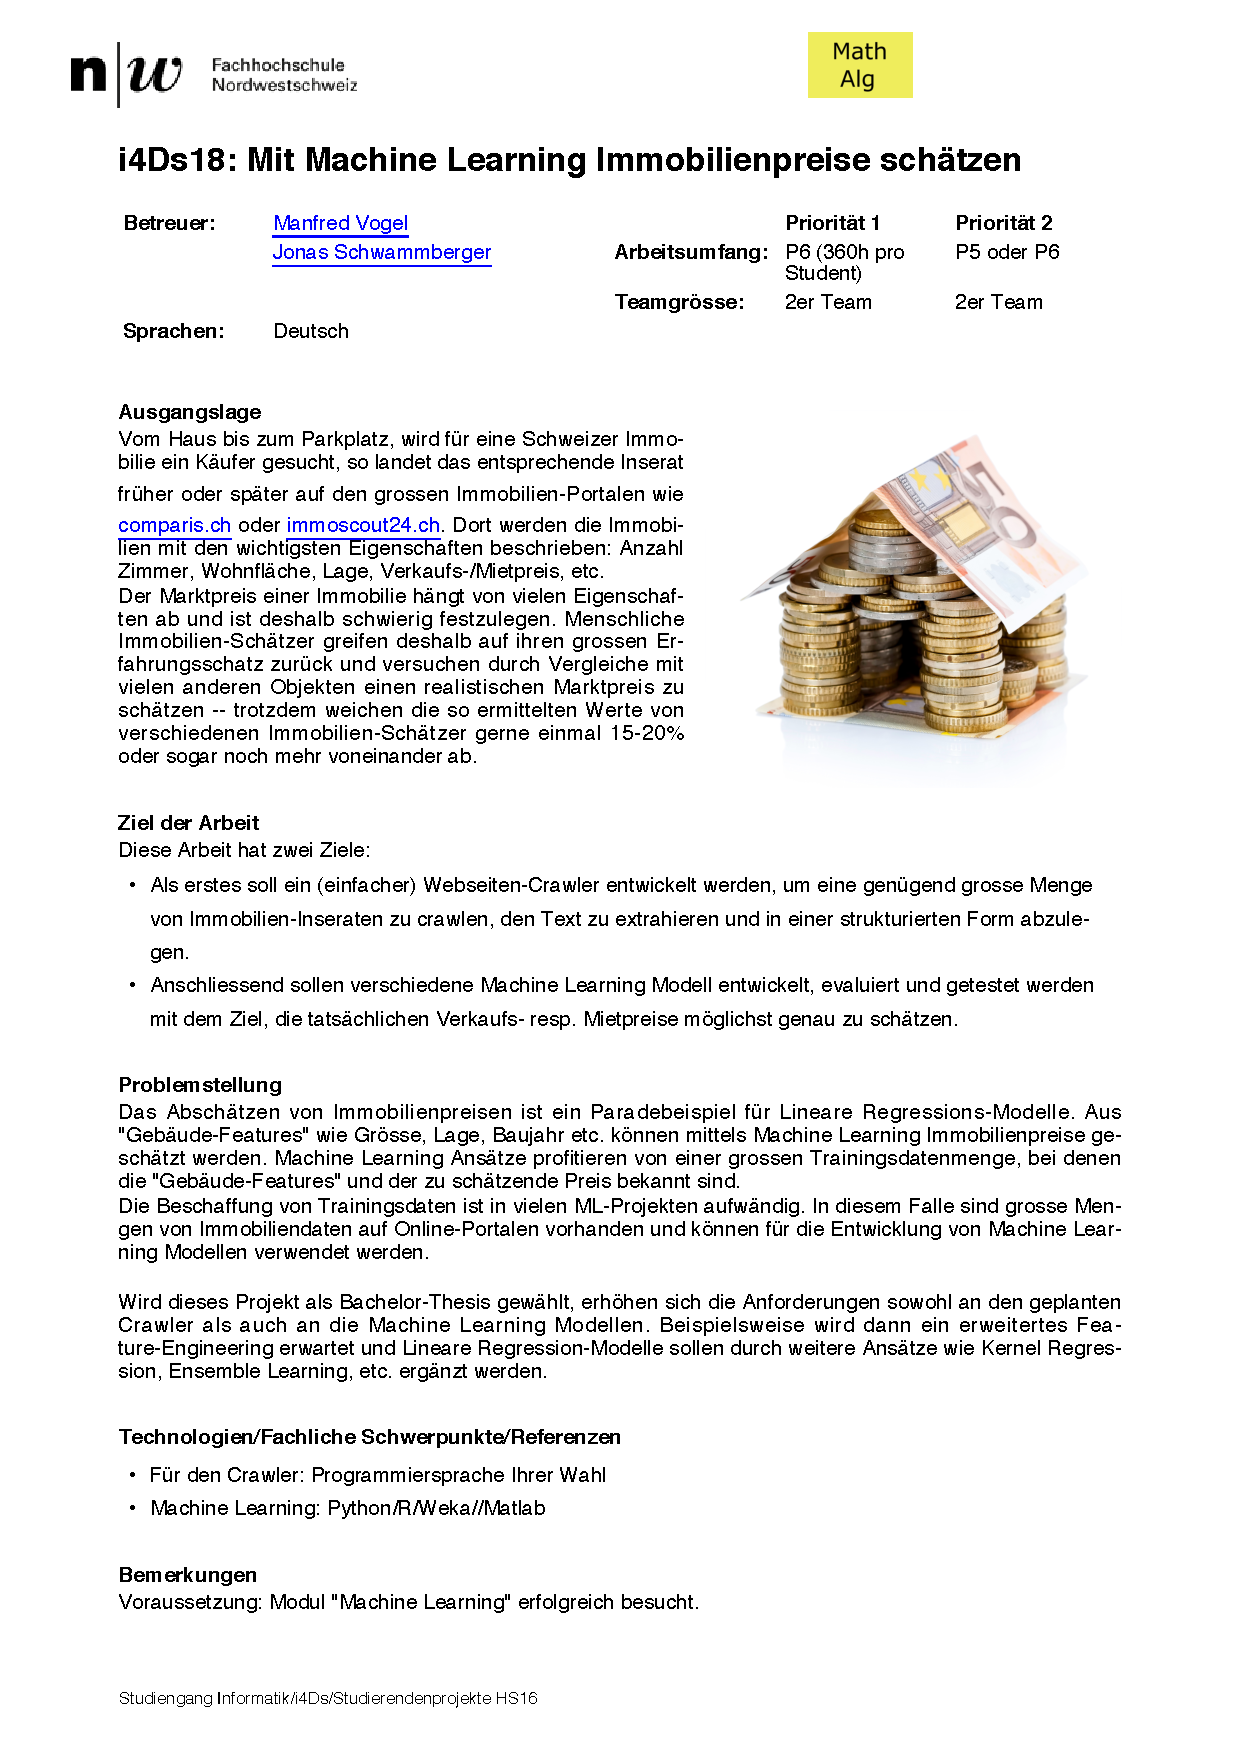
\includegraphics[trim={1.5cm 2.3cm 1.5cm 2.5cm},clip,width=\textwidth]{attachments/ausschreibung.pdf}
\newpage
\subsection{Crawler}
\label{crawler_a}
Tabelle \ref{tab:crawled_info} zeigt alle gesammelten Informationen eines Inserates.

\begin{table*}[ht]
  \centering
  \ra{1.3}
  \resizebox{\textwidth}{!}{
  \begin{tabular}{@{}ll@{}}
  \toprule
  Kennwert & Beschreibung\\
  \midrule
  object\_id & Objektid der Plattform zur Wiedererkennung.\\
  reference\_no & Offizielle Referenznummer. \\
  raw\_data & Die ganze Seite als HTML.\\
  crawler & Name der Plattform.\\
  url & URL zum Inserat.\\
  available & Ist es noch zu kaufen.\\
  street & Strassenanschrift der Immobilie.\\
  place & PLZ und Ortschaft der Immobilie.\\
  price\_brutto & Gesamter Kaufpreis der Immobilie.\\
  price\_netto & Nettopreis der Immobilie.\\
  additional\_costs & Zusätzliche Kosten für diverse Sachen.\\
  description & Die Beschreibung der Immobbilie.\\
  living\_area & Die Wohnflöche der Immobilie.\\
  floor & Auf welchem Stockwerk sich die Immobilie befindet.\\
  num\_rooms & Die Anzahl an Zimmer die die Immobilie besitzt.\\
  num\_floors & Die Anzahl an Stockwerken die die Immobbilie besitzt.\\
  build\_year & Baujahr der Immobilie.\\
  last\_renovation\_year & Letztes Renovationsjahr der Immobilie.\\
  cubature & Die Kubatur der Immobilie.\\
  room\_height & Die Raumhöhe der Immobilie.\\
  effective\_area & Die Nutzfläche oder effektive Fläche der Immobile.\\
  plot\_area & Die Grundstückfläche auf der die Immobilie liegt.\\
  floors\_house & Die Anzahl an Stockwerken insgesamt, die diese Immobilie besitzt.\\
  characteristics & Zusätzliche Merkmale der Imobilie.\\
  additional\_data & Daten die noch nicht zugeordnet werden können, aber die Immobilie beschreiben.\\
  owner  & Besitzer der Immobilie.\\
  objecttype & Objekttyp\\
  condition & In welchem Zustand sich die Immobilie befindet.\\
  longitude & Longitude Koordinate für die Lärmbelastungsberechnung.\\
  latitude & Latitude Koordinate für die Lärmbelastungsberechnung.\\
  quality\_label & Welches Qualitätslabel die Immobilie besitzt.\\
  \bottomrule
\end{tabular}}
\caption{Gesammelten Informationen eines Inserates}
\label{tab:crawled_info}
\end{table*}

\subsection{Datenanlyse}
\label{daten_analys}
Im folgenden werden alle Diagramme angezeigt die bei der Analyse der Daten erstellt und verwendet wurden.

\begin{figure}[h]
\begin{subfigure}{.5\textwidth}
  \centering
  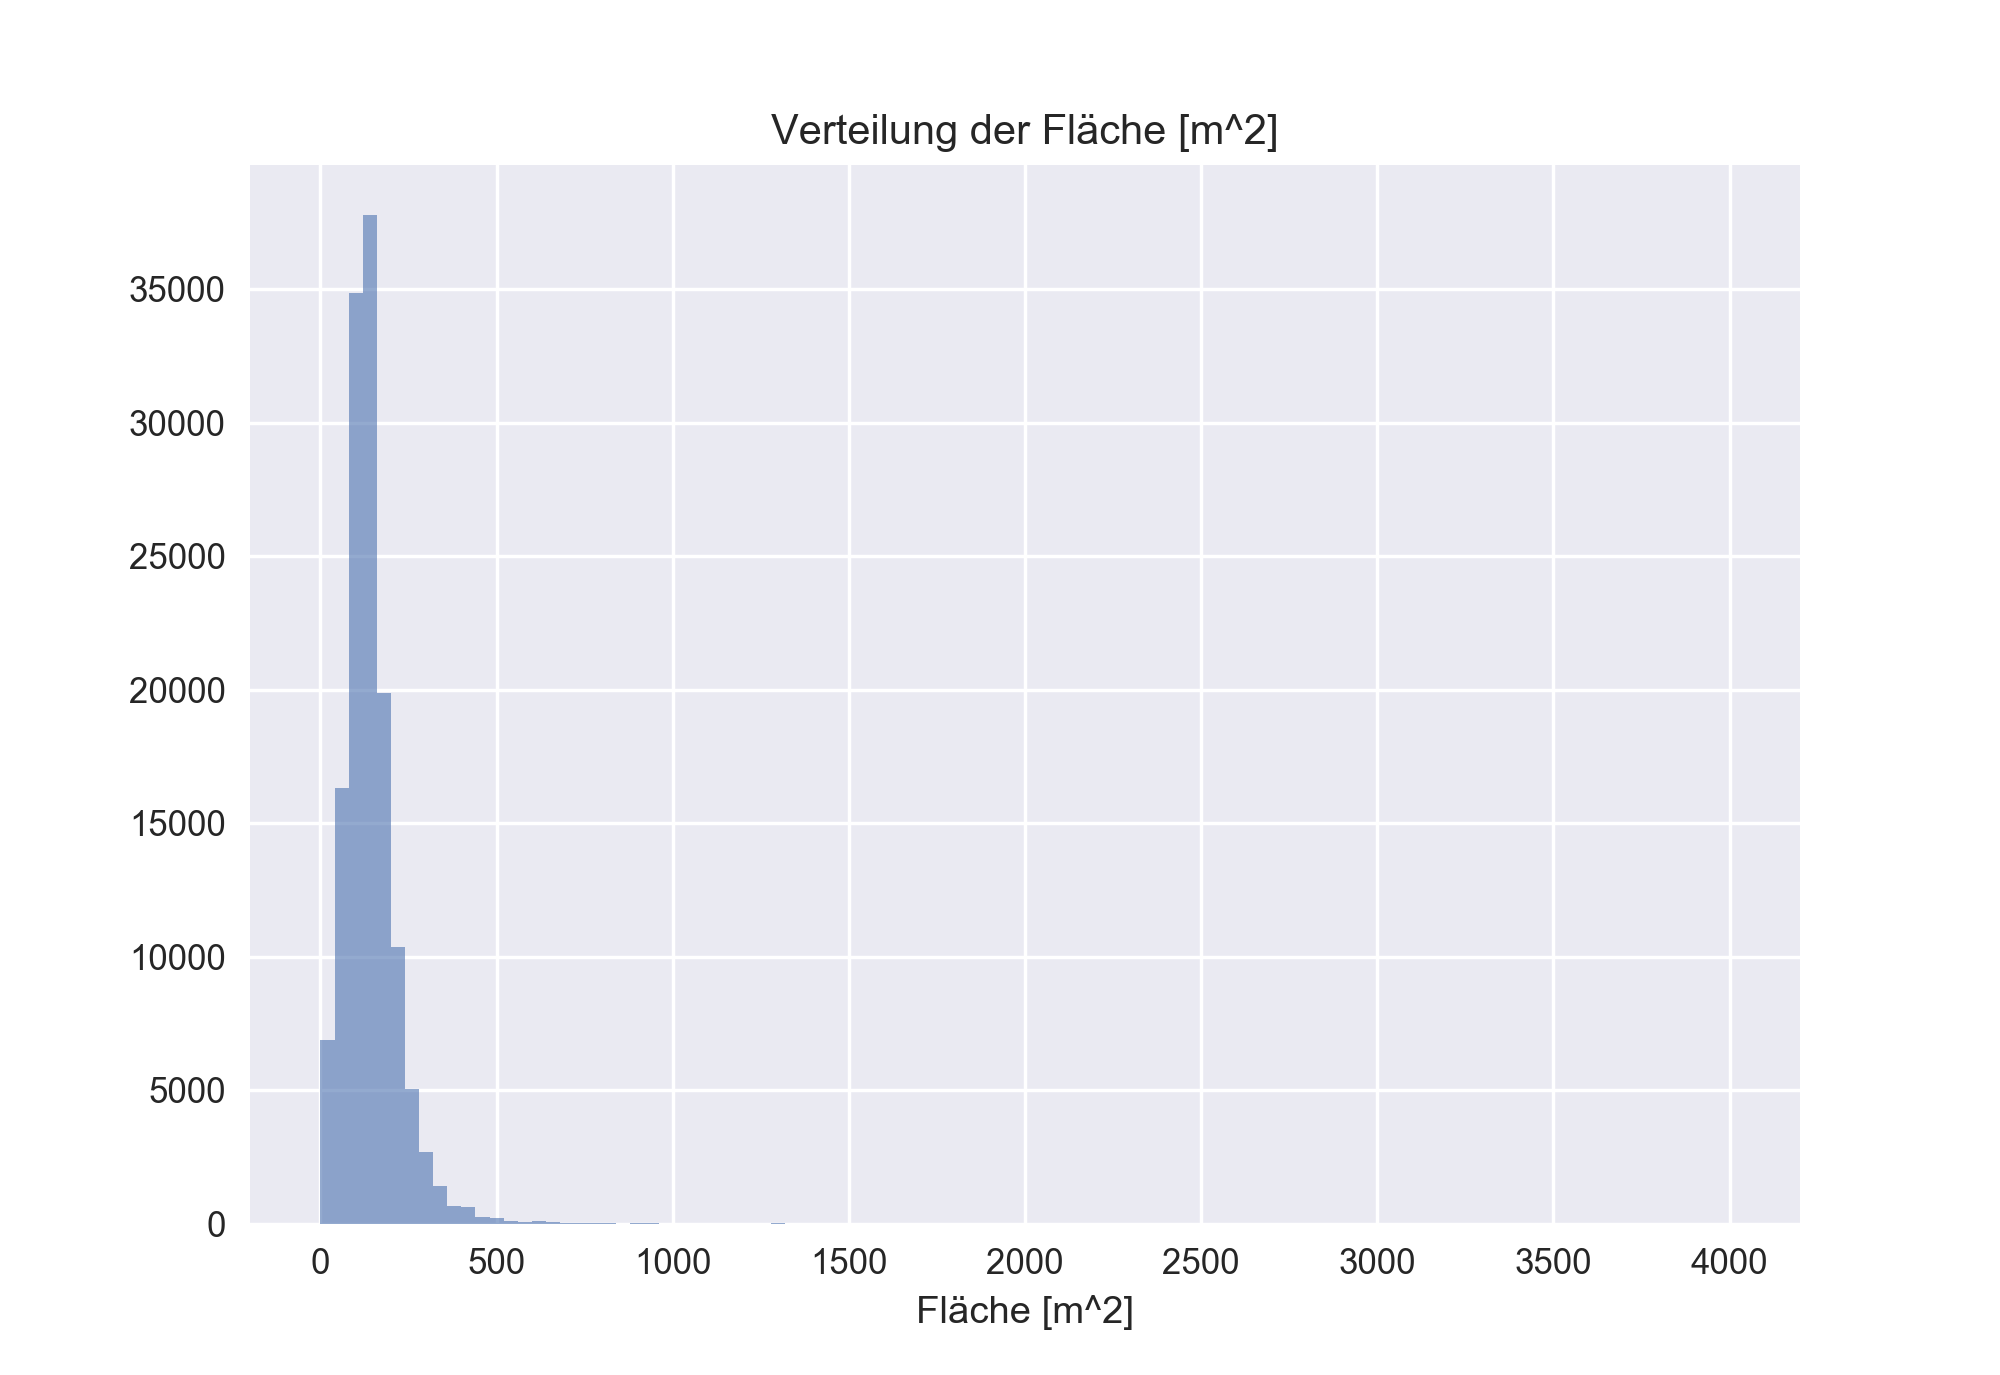
\includegraphics[width=\linewidth]{images/anhang/analysis/Verteilung_living_area.png}
  \caption{Verteilung der Wohnfläche}
\end{subfigure}
\begin{subfigure}{.5\textwidth}
  \centering
  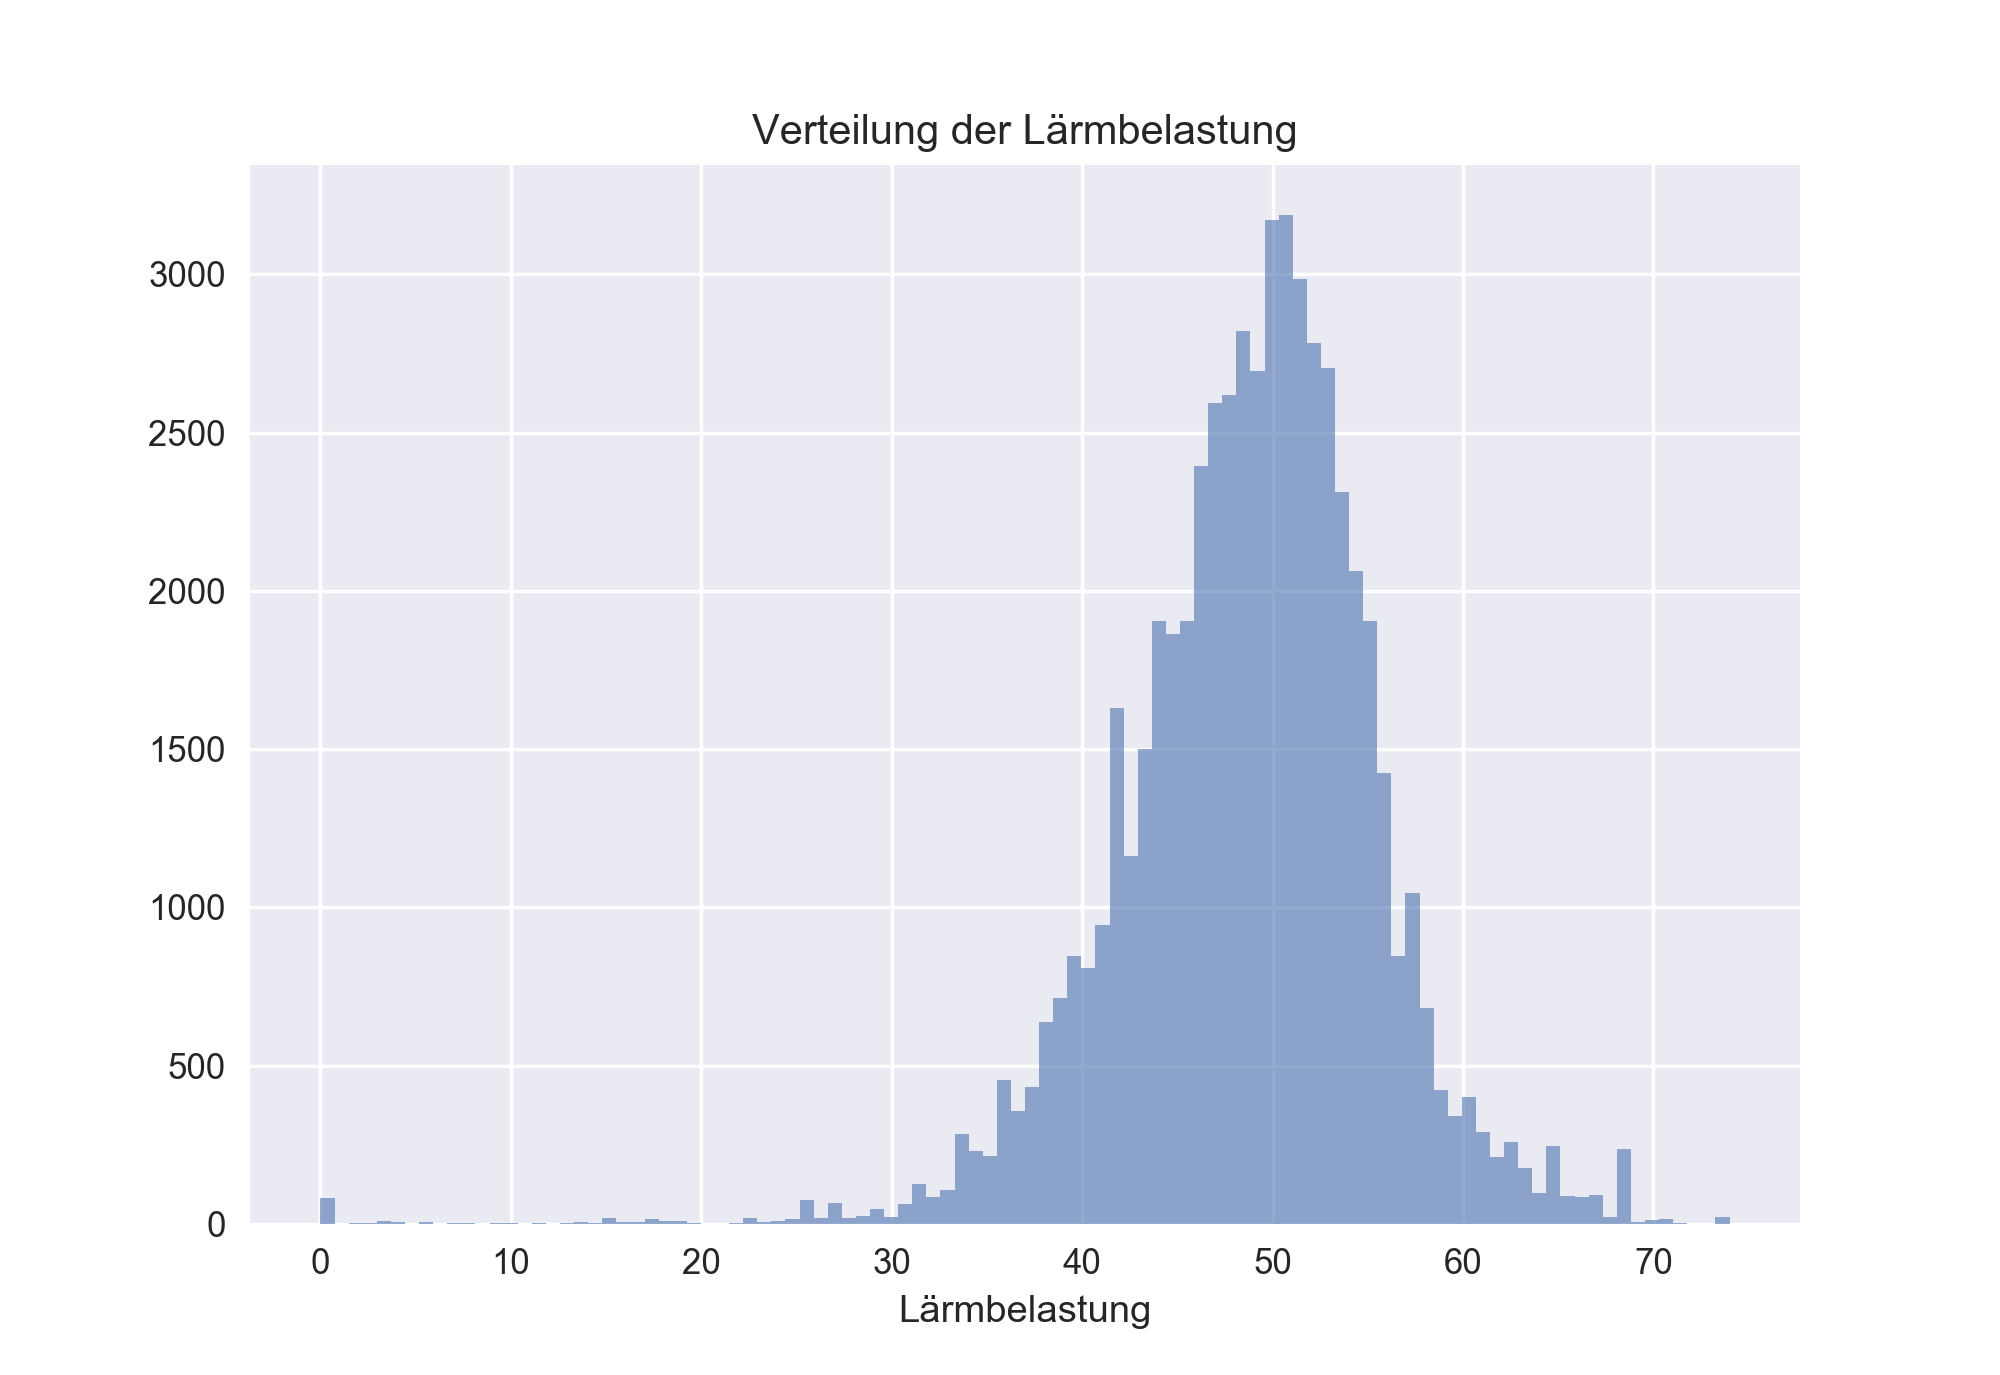
\includegraphics[width=\linewidth]{images/anhang/analysis/Verteilung_noise_level.png}
  \caption{Verteilung der Lärmbelastung} 
\end{subfigure}
\begin{subfigure}{.5\textwidth}
  \centering
  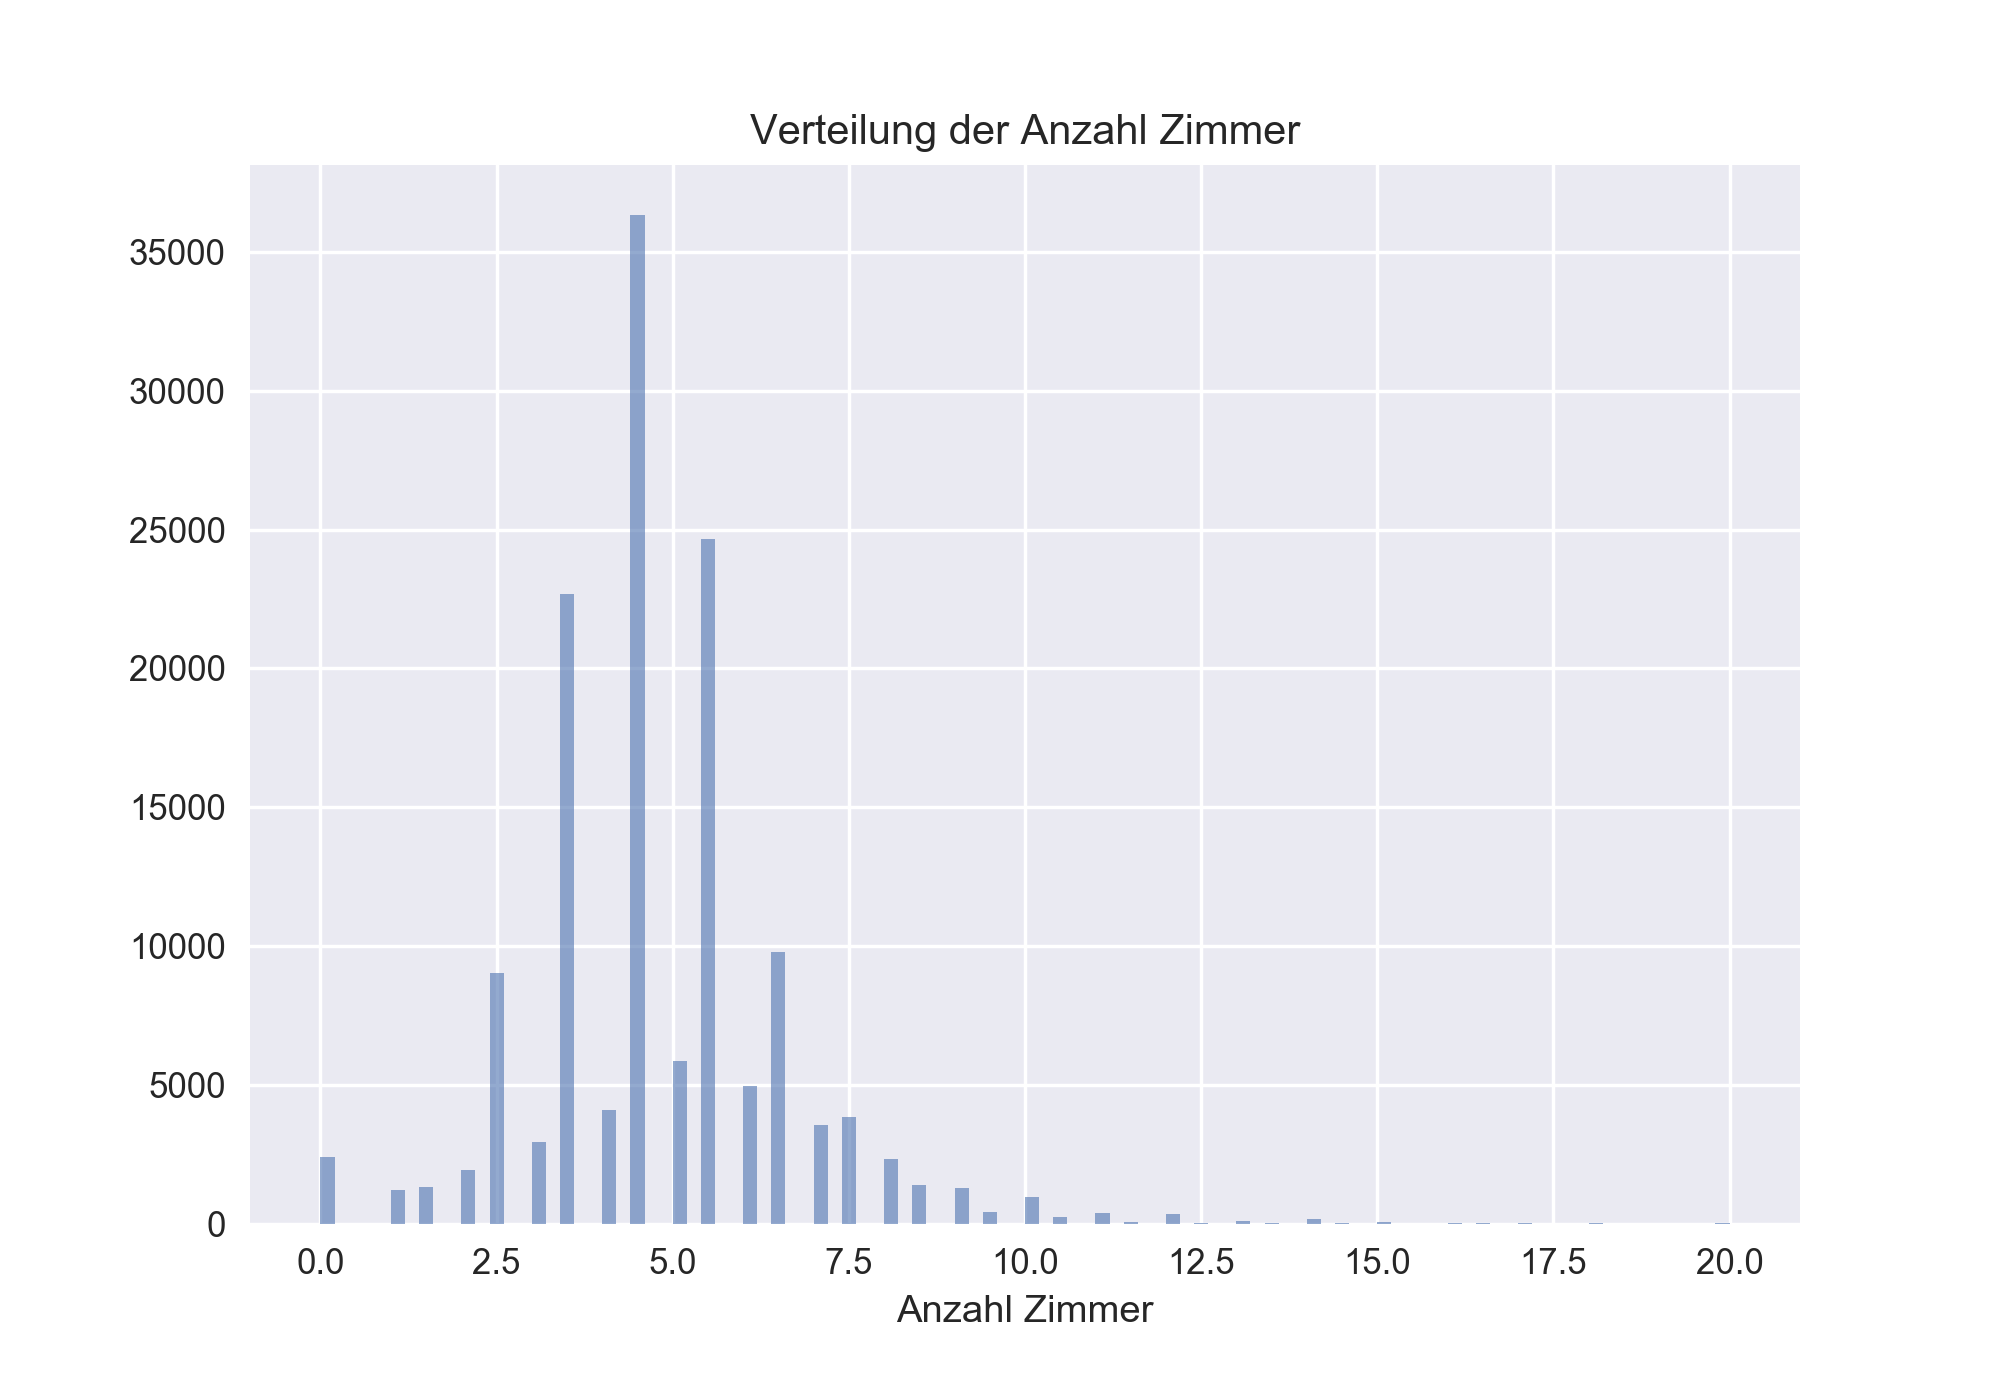
\includegraphics[width=\linewidth]{images/anhang/analysis/Verteilung_num_rooms.png}
  \caption{Verteilung der Anzahl Zimmer}
\end{subfigure}
\caption{Verteilung der nummerischen Werten}
\end{figure}

\begin{figure}[H]
\begin{subfigure}{.5\textwidth}
  \centering
  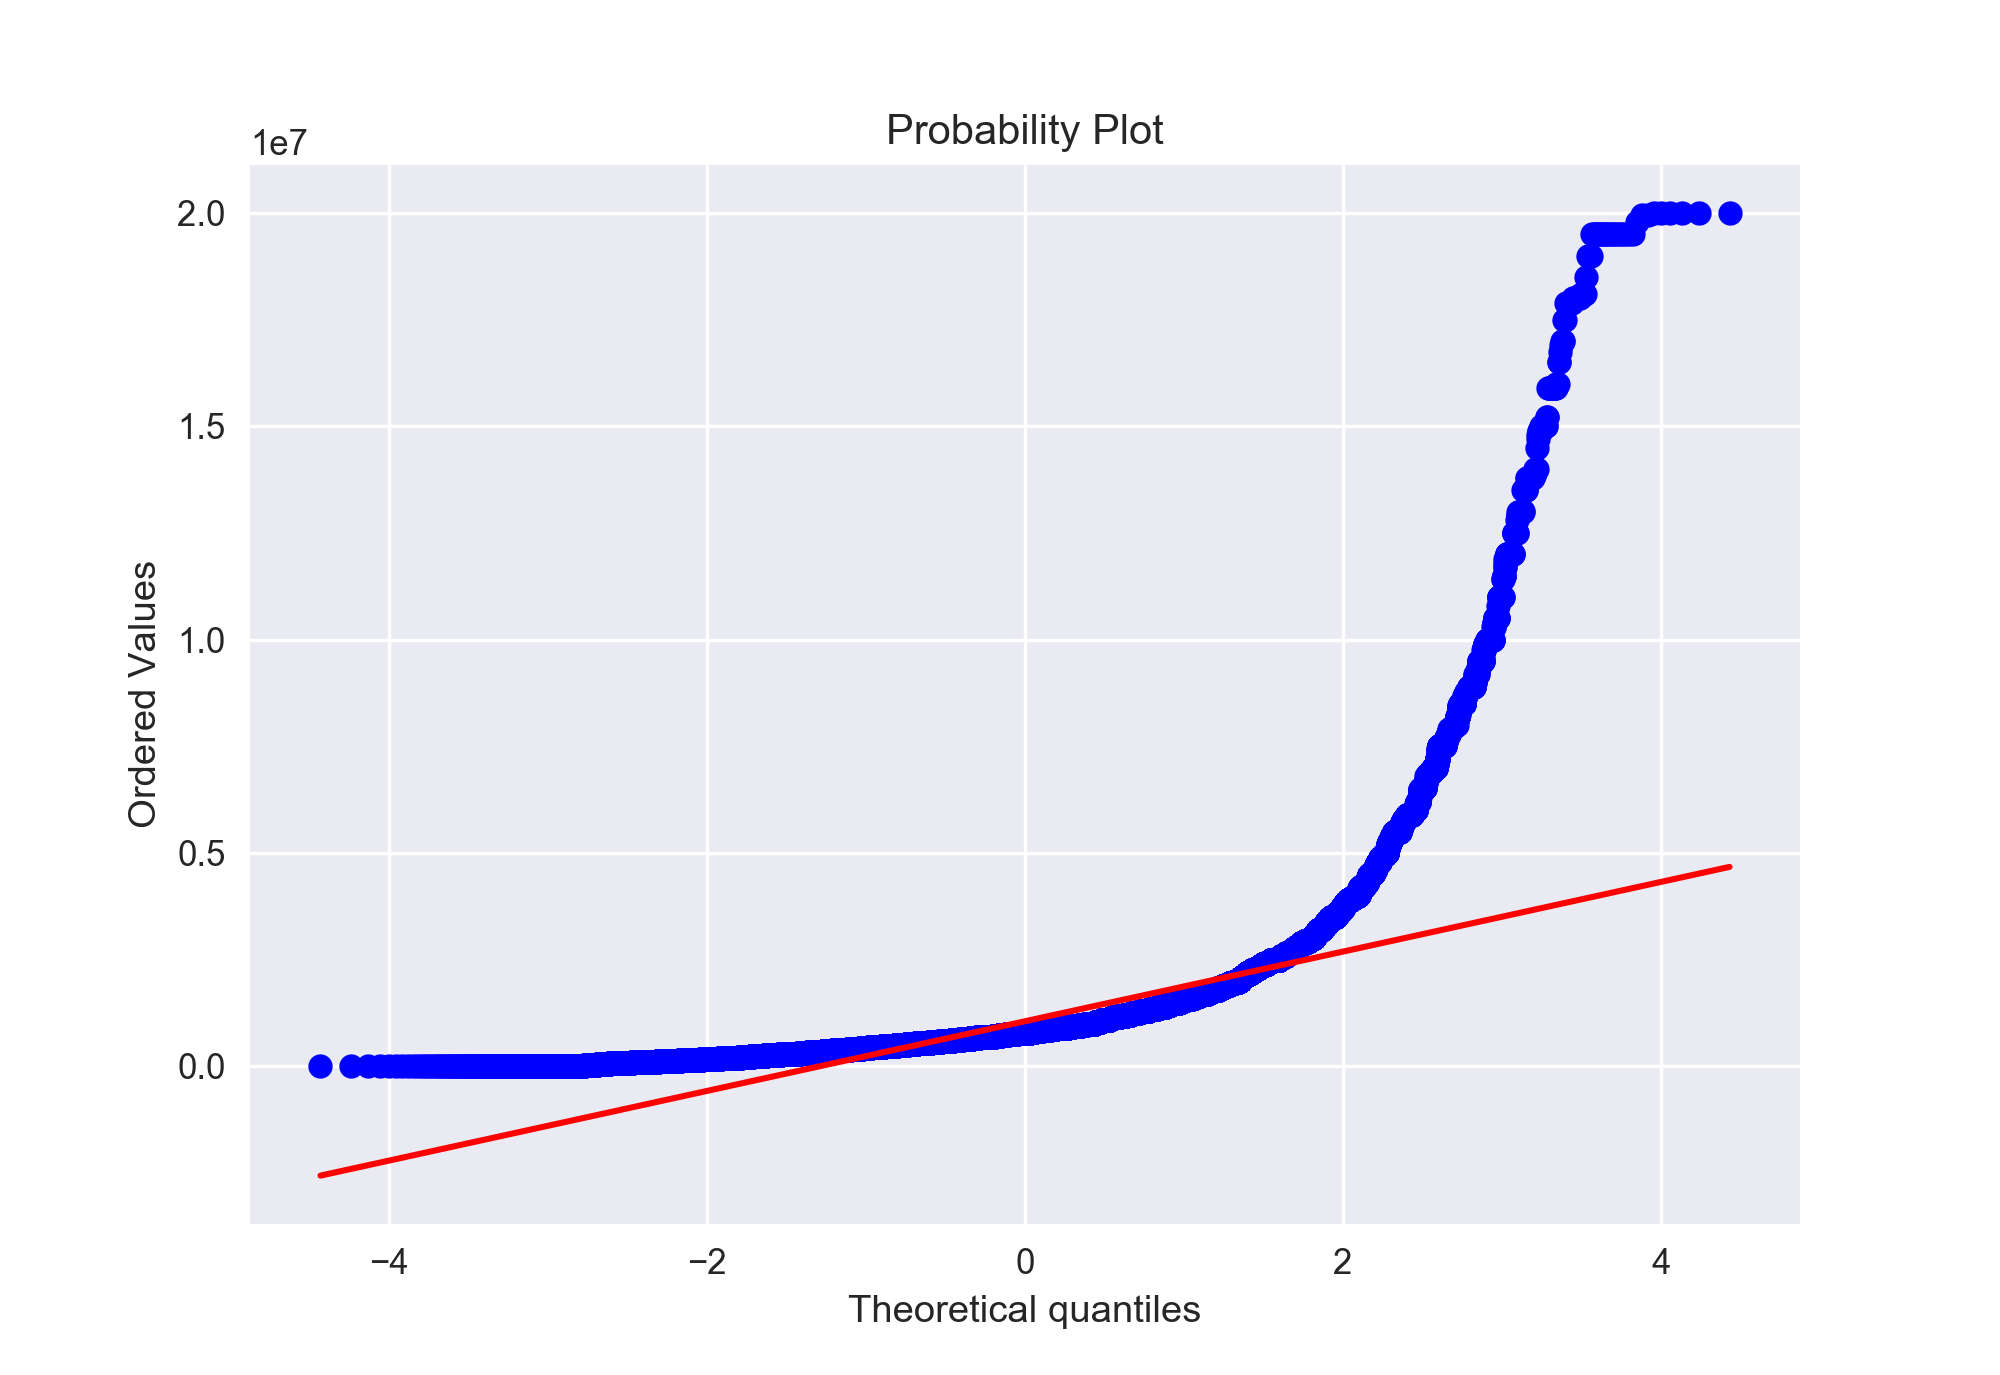
\includegraphics[width=\linewidth]{images/anhang/analysis/skewness.png}
  \caption{Preis - Skewness}
\end{subfigure}
\begin{subfigure}{.5\textwidth}
  \centering
  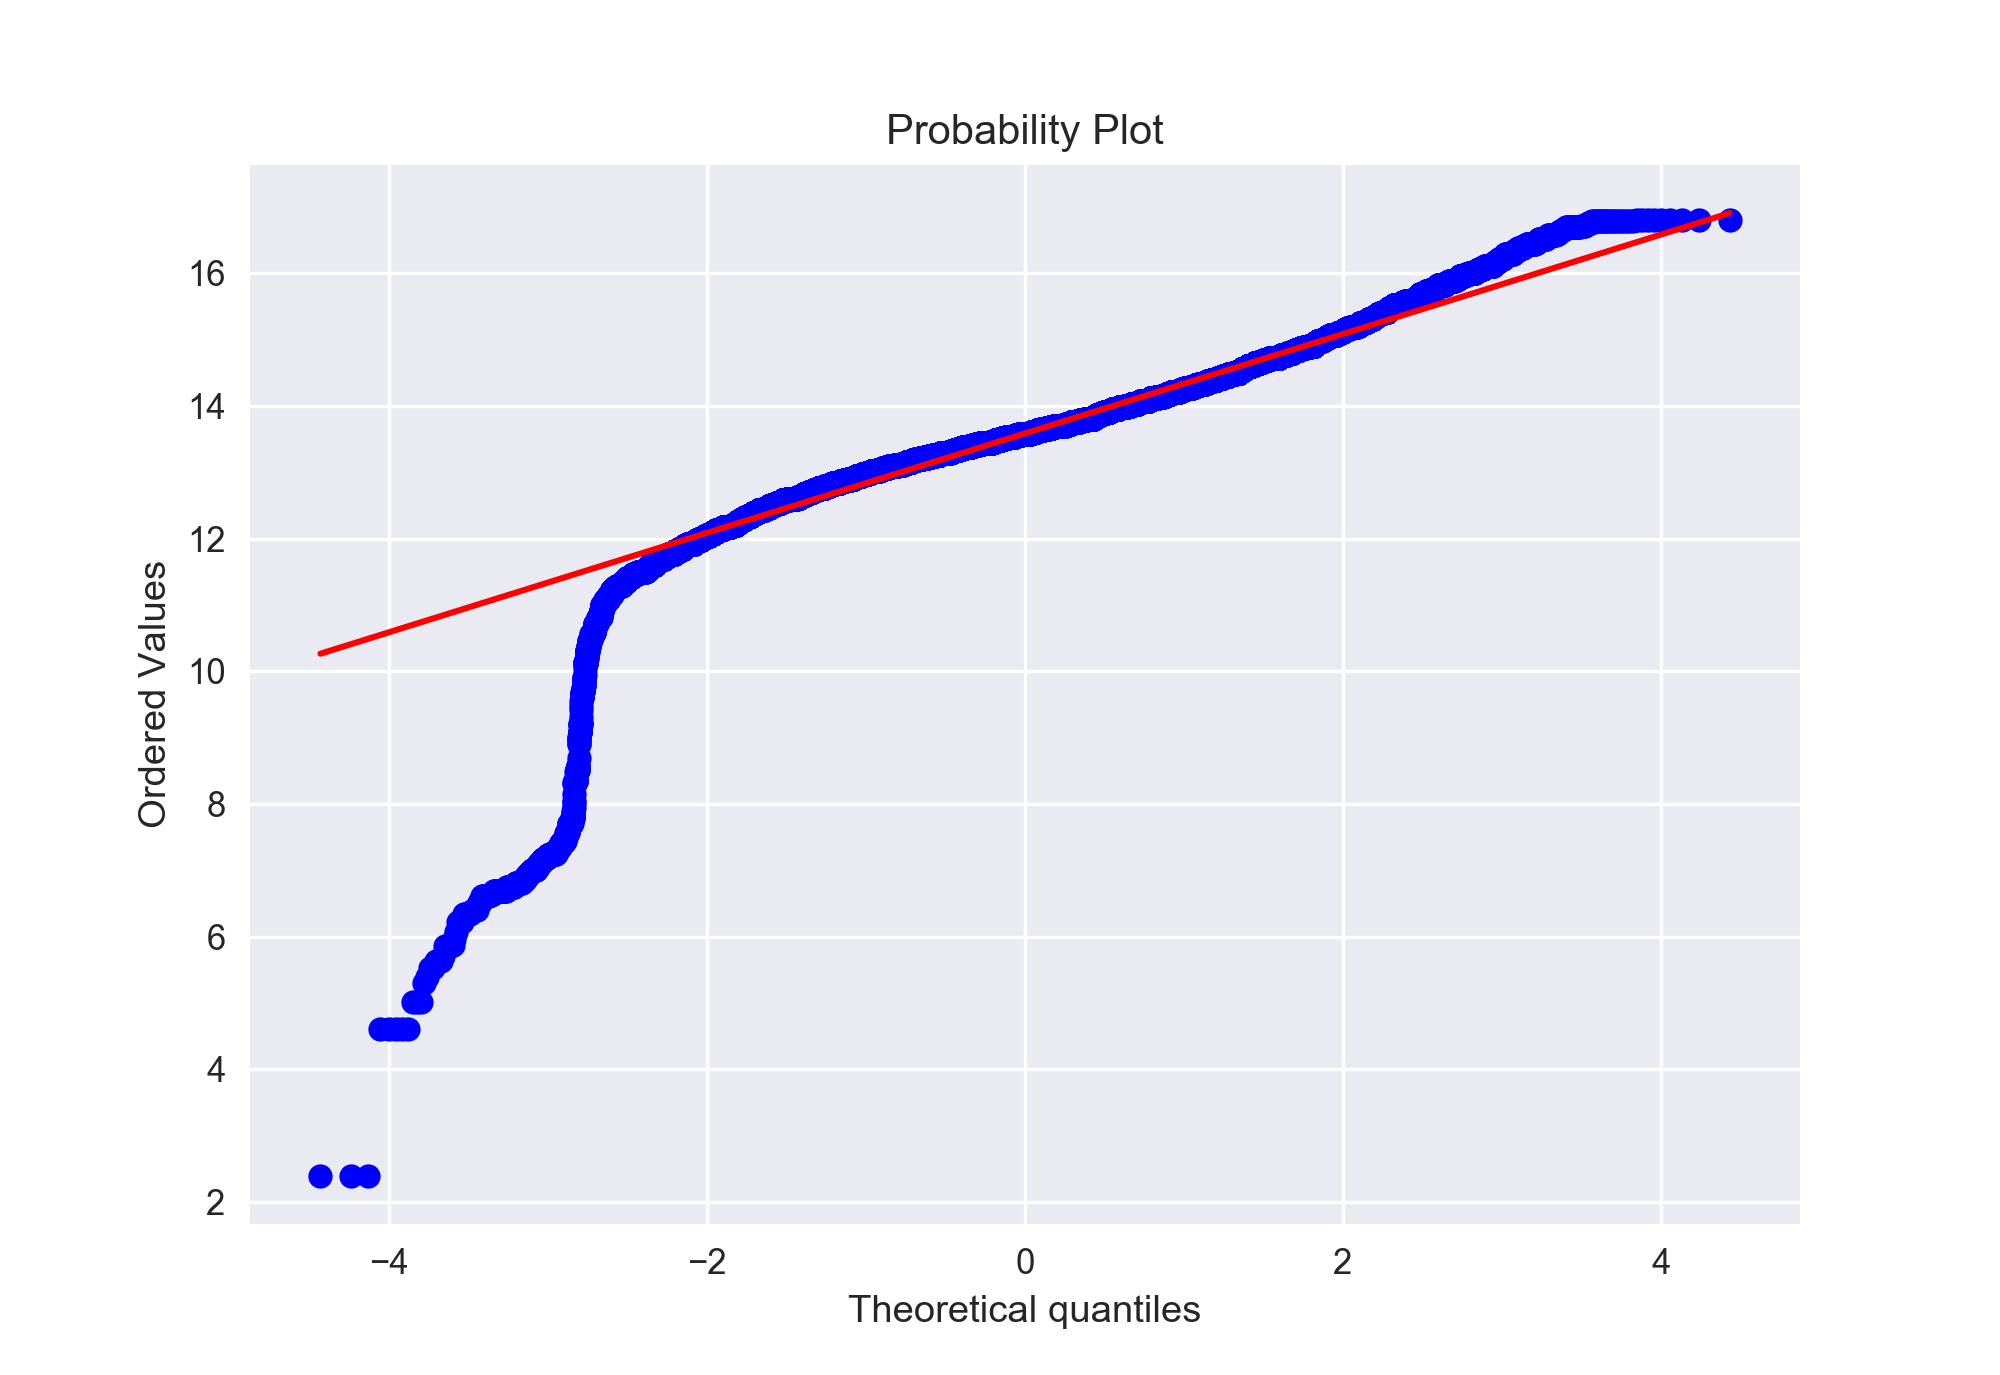
\includegraphics[width=\linewidth]{images/anhang/analysis/log_skewness.png}
  \caption{Preis - Skewness mit Log} 
\end{subfigure}
\caption{Preisanalyse}
\end{figure}

\begin{figure}[h]
\begin{subfigure}{.5\textwidth}
  \centering
  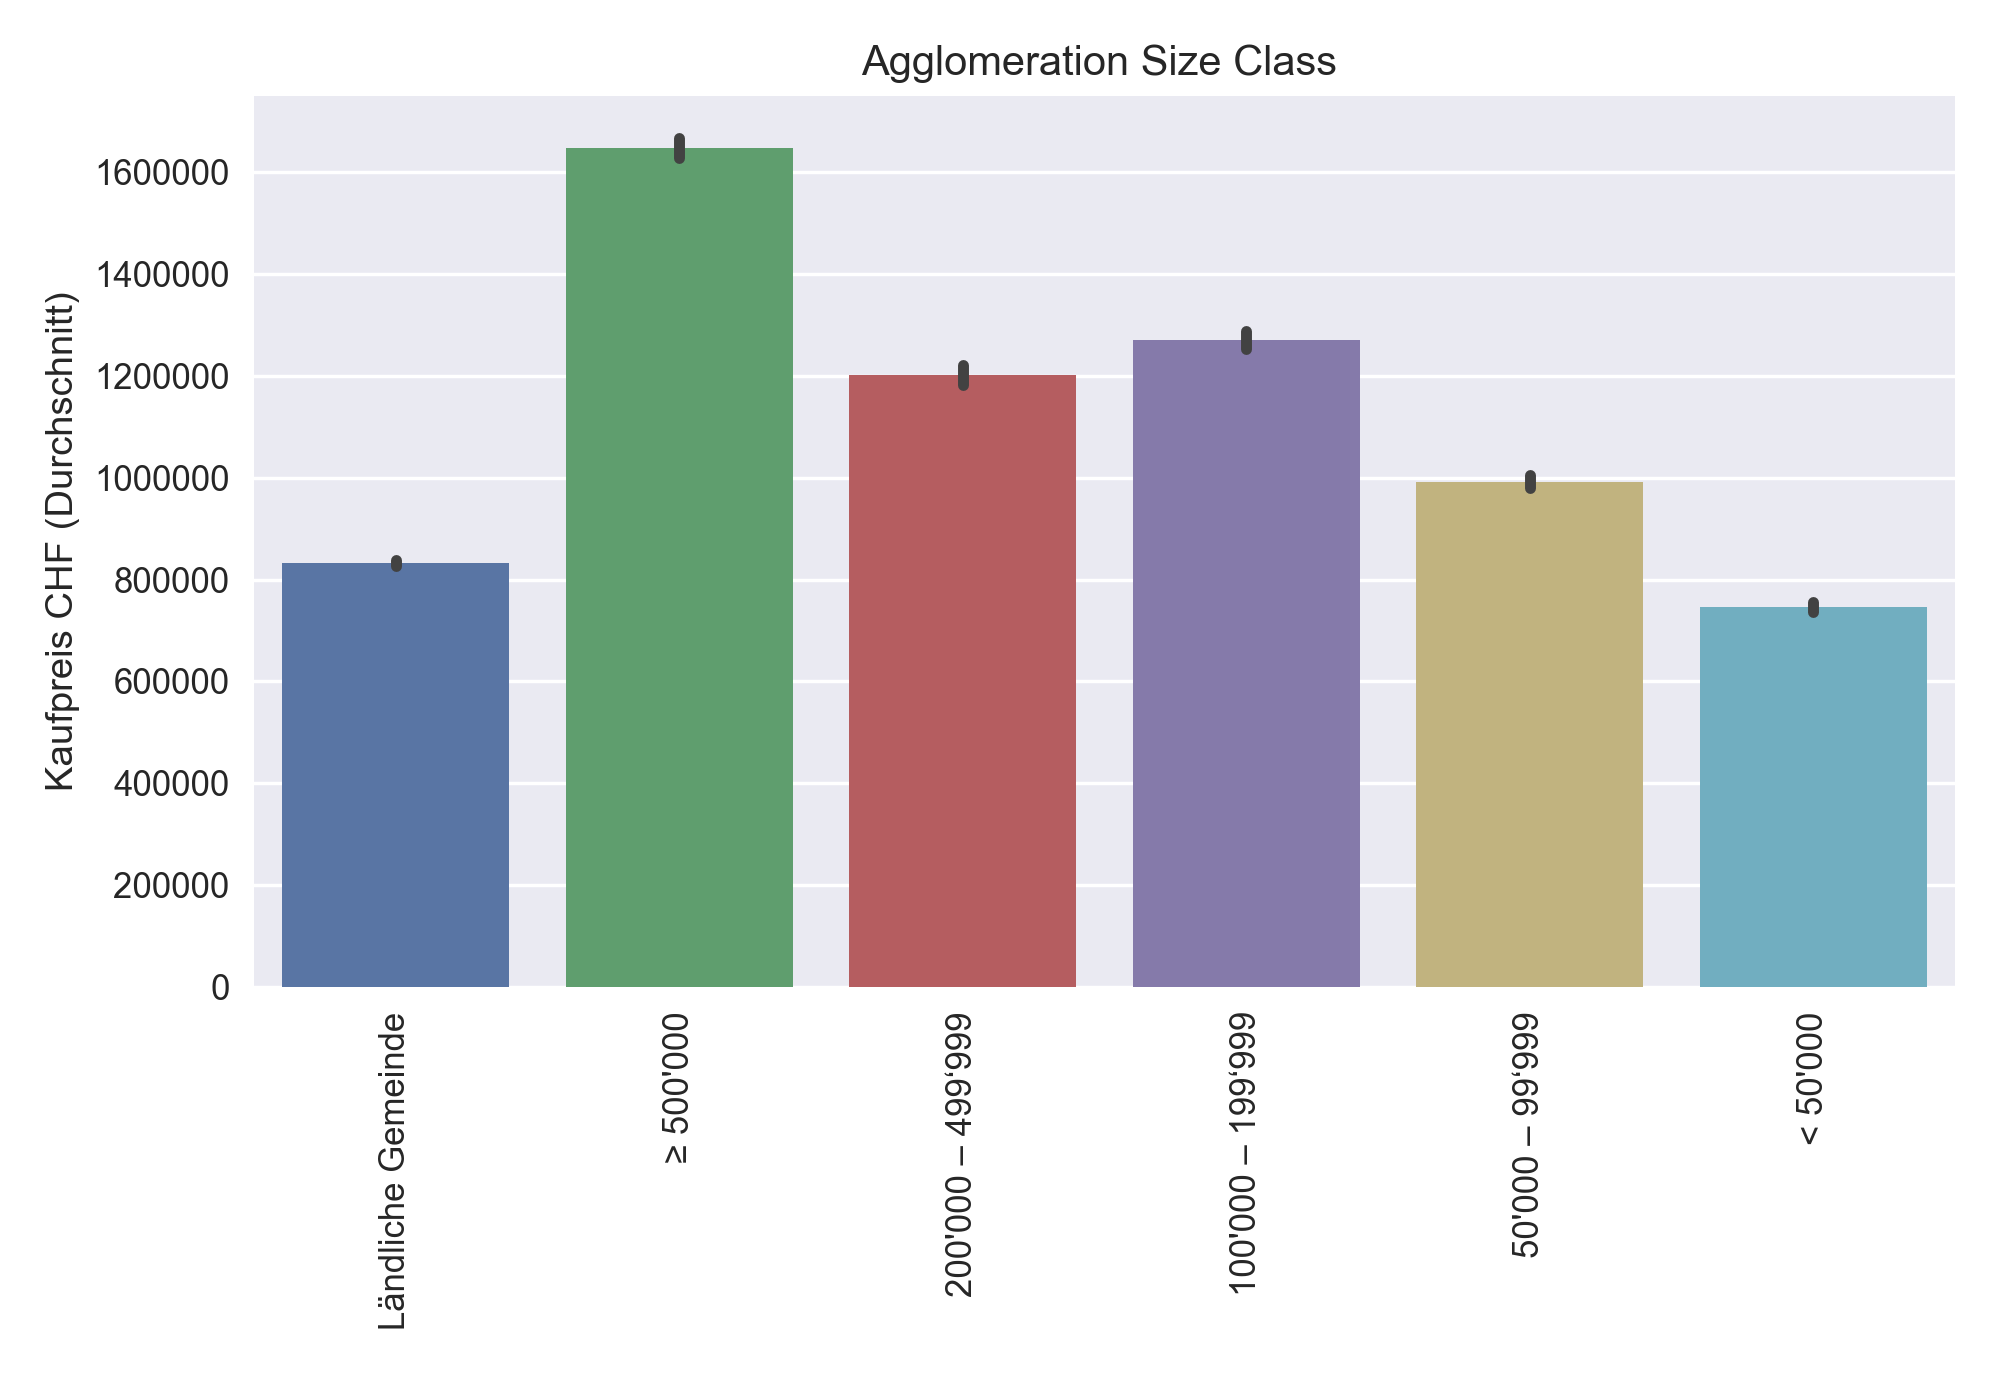
\includegraphics[width=\linewidth]{images/anhang/analysis/barplot_agglomeration_size_class_id.png}
  \caption{Agglomerationsgrössen}
\end{subfigure}
\begin{subfigure}{.5\textwidth}
  \centering
  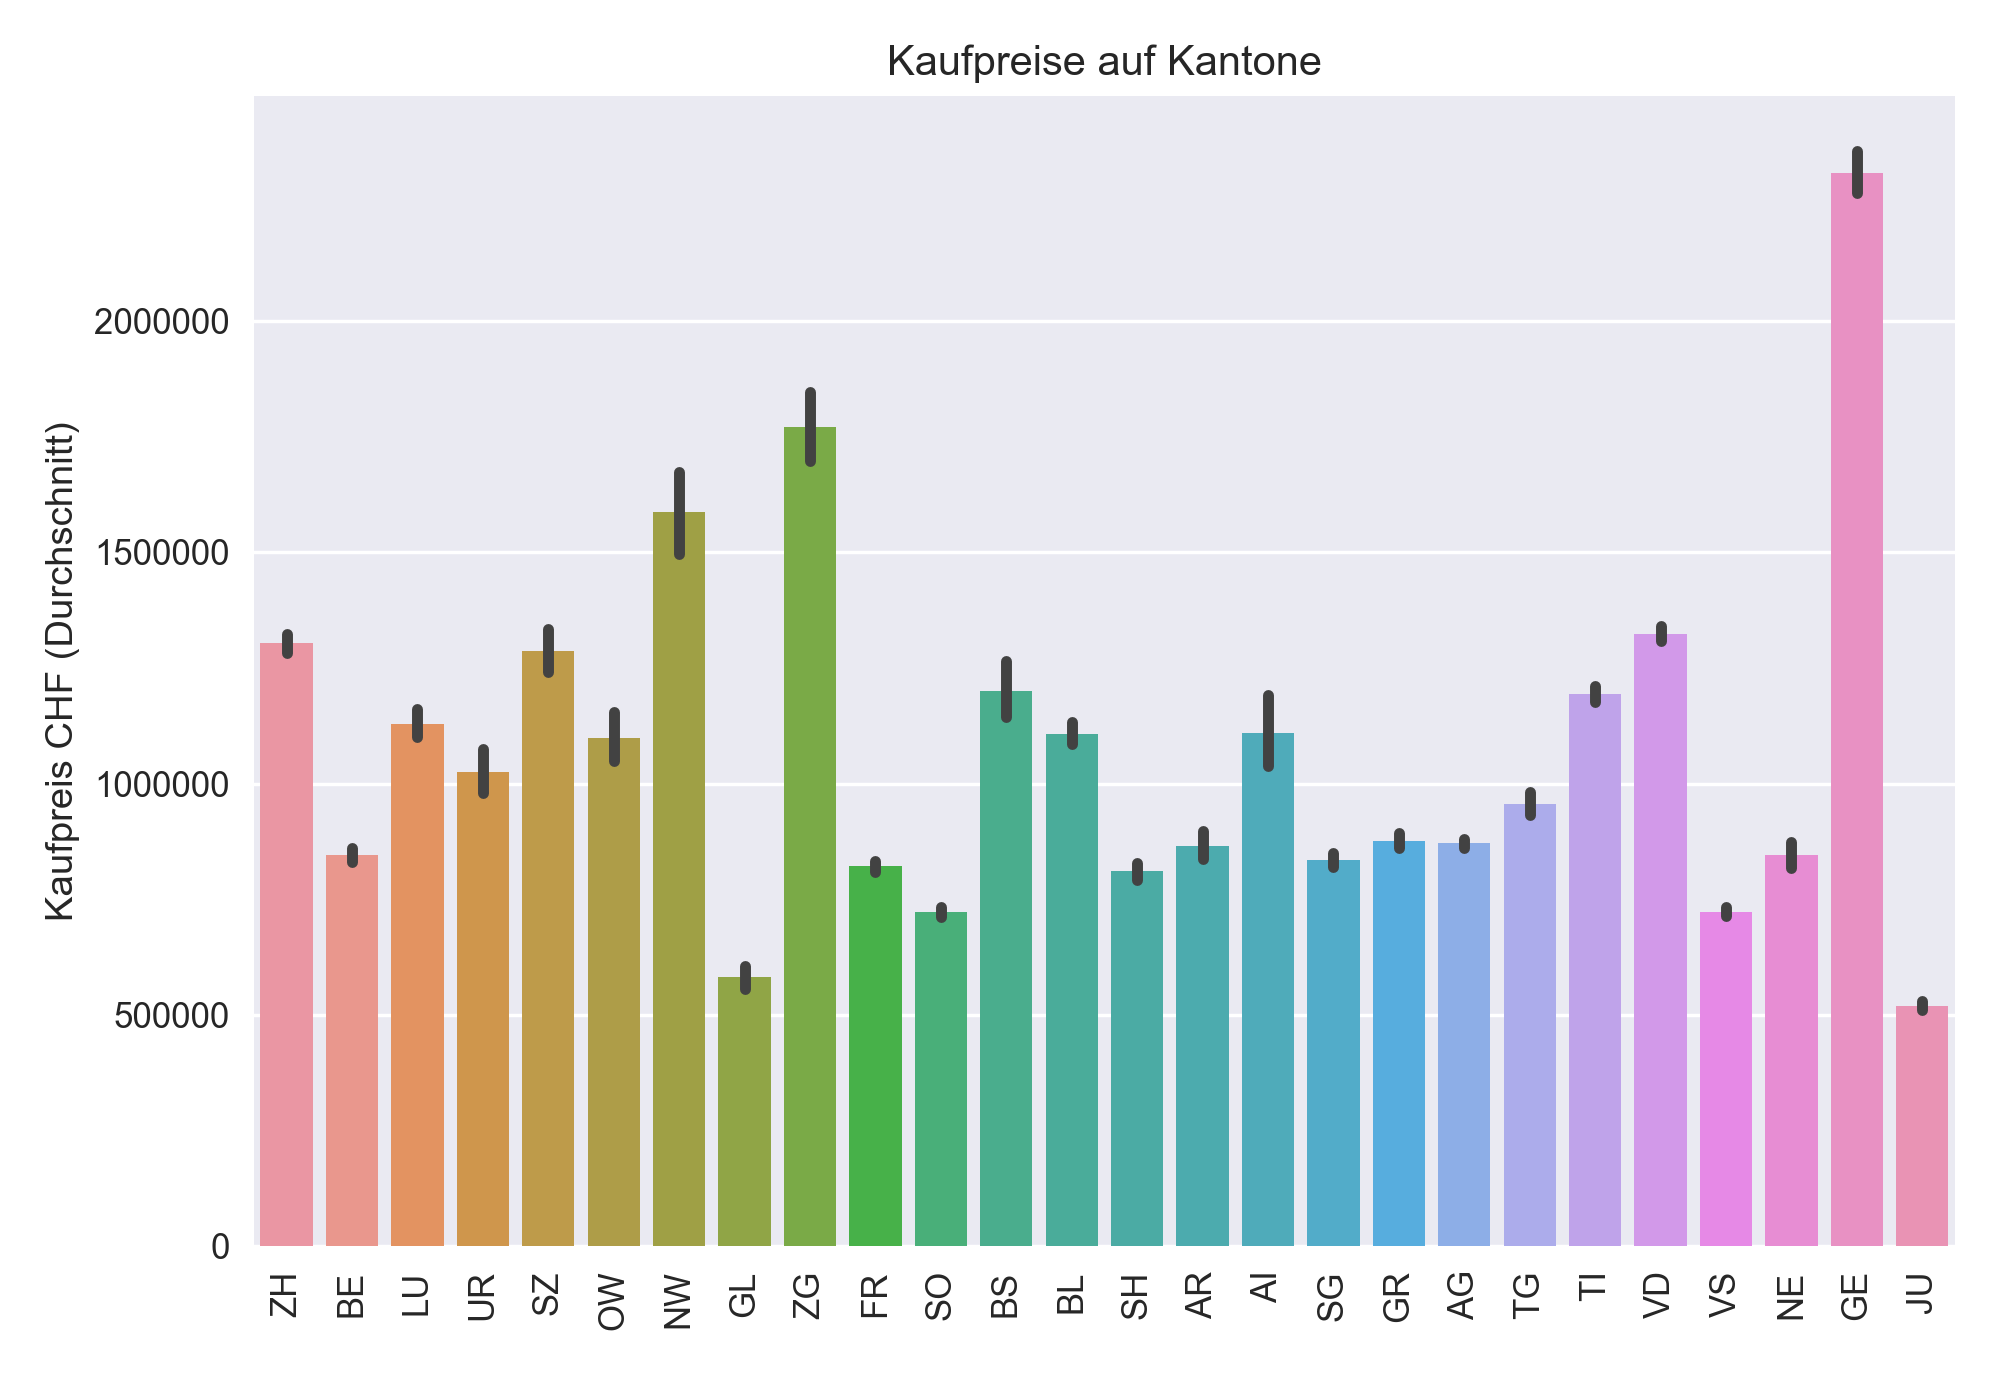
\includegraphics[width=\linewidth]{images/anhang/analysis/barplot_canton.png}
  \caption{Kanton} 
\end{subfigure}
\begin{subfigure}{.5\textwidth}
  \centering
  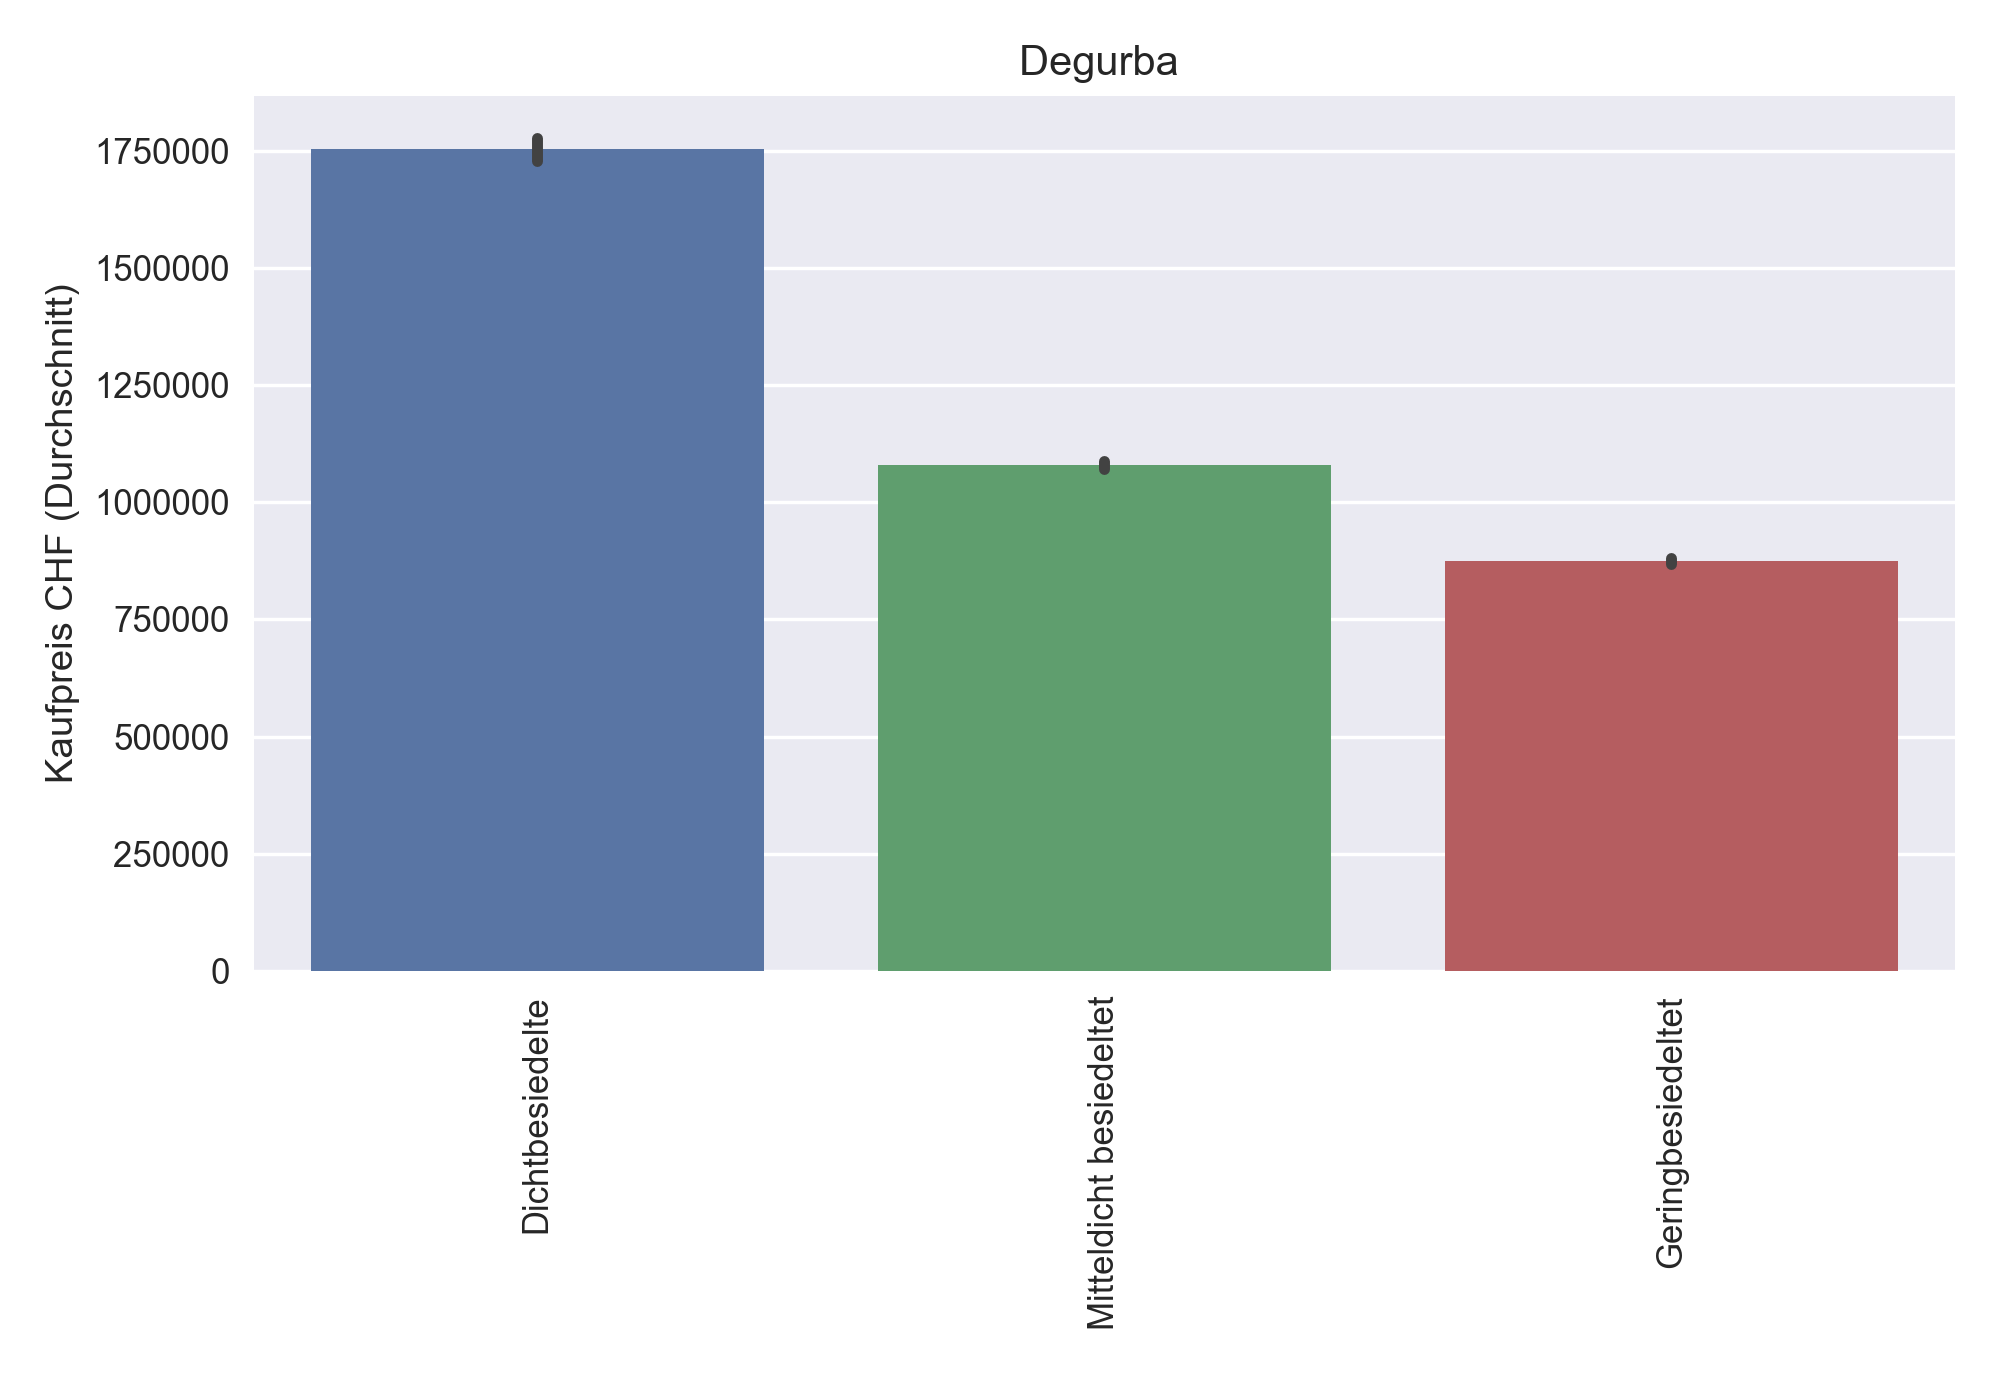
\includegraphics[width=\linewidth]{images/anhang/analysis/barplot_degurba_id.png}
  \caption{Grad der Urbanisierung} 
\end{subfigure}
\begin{subfigure}{.5\textwidth}
  \centering
  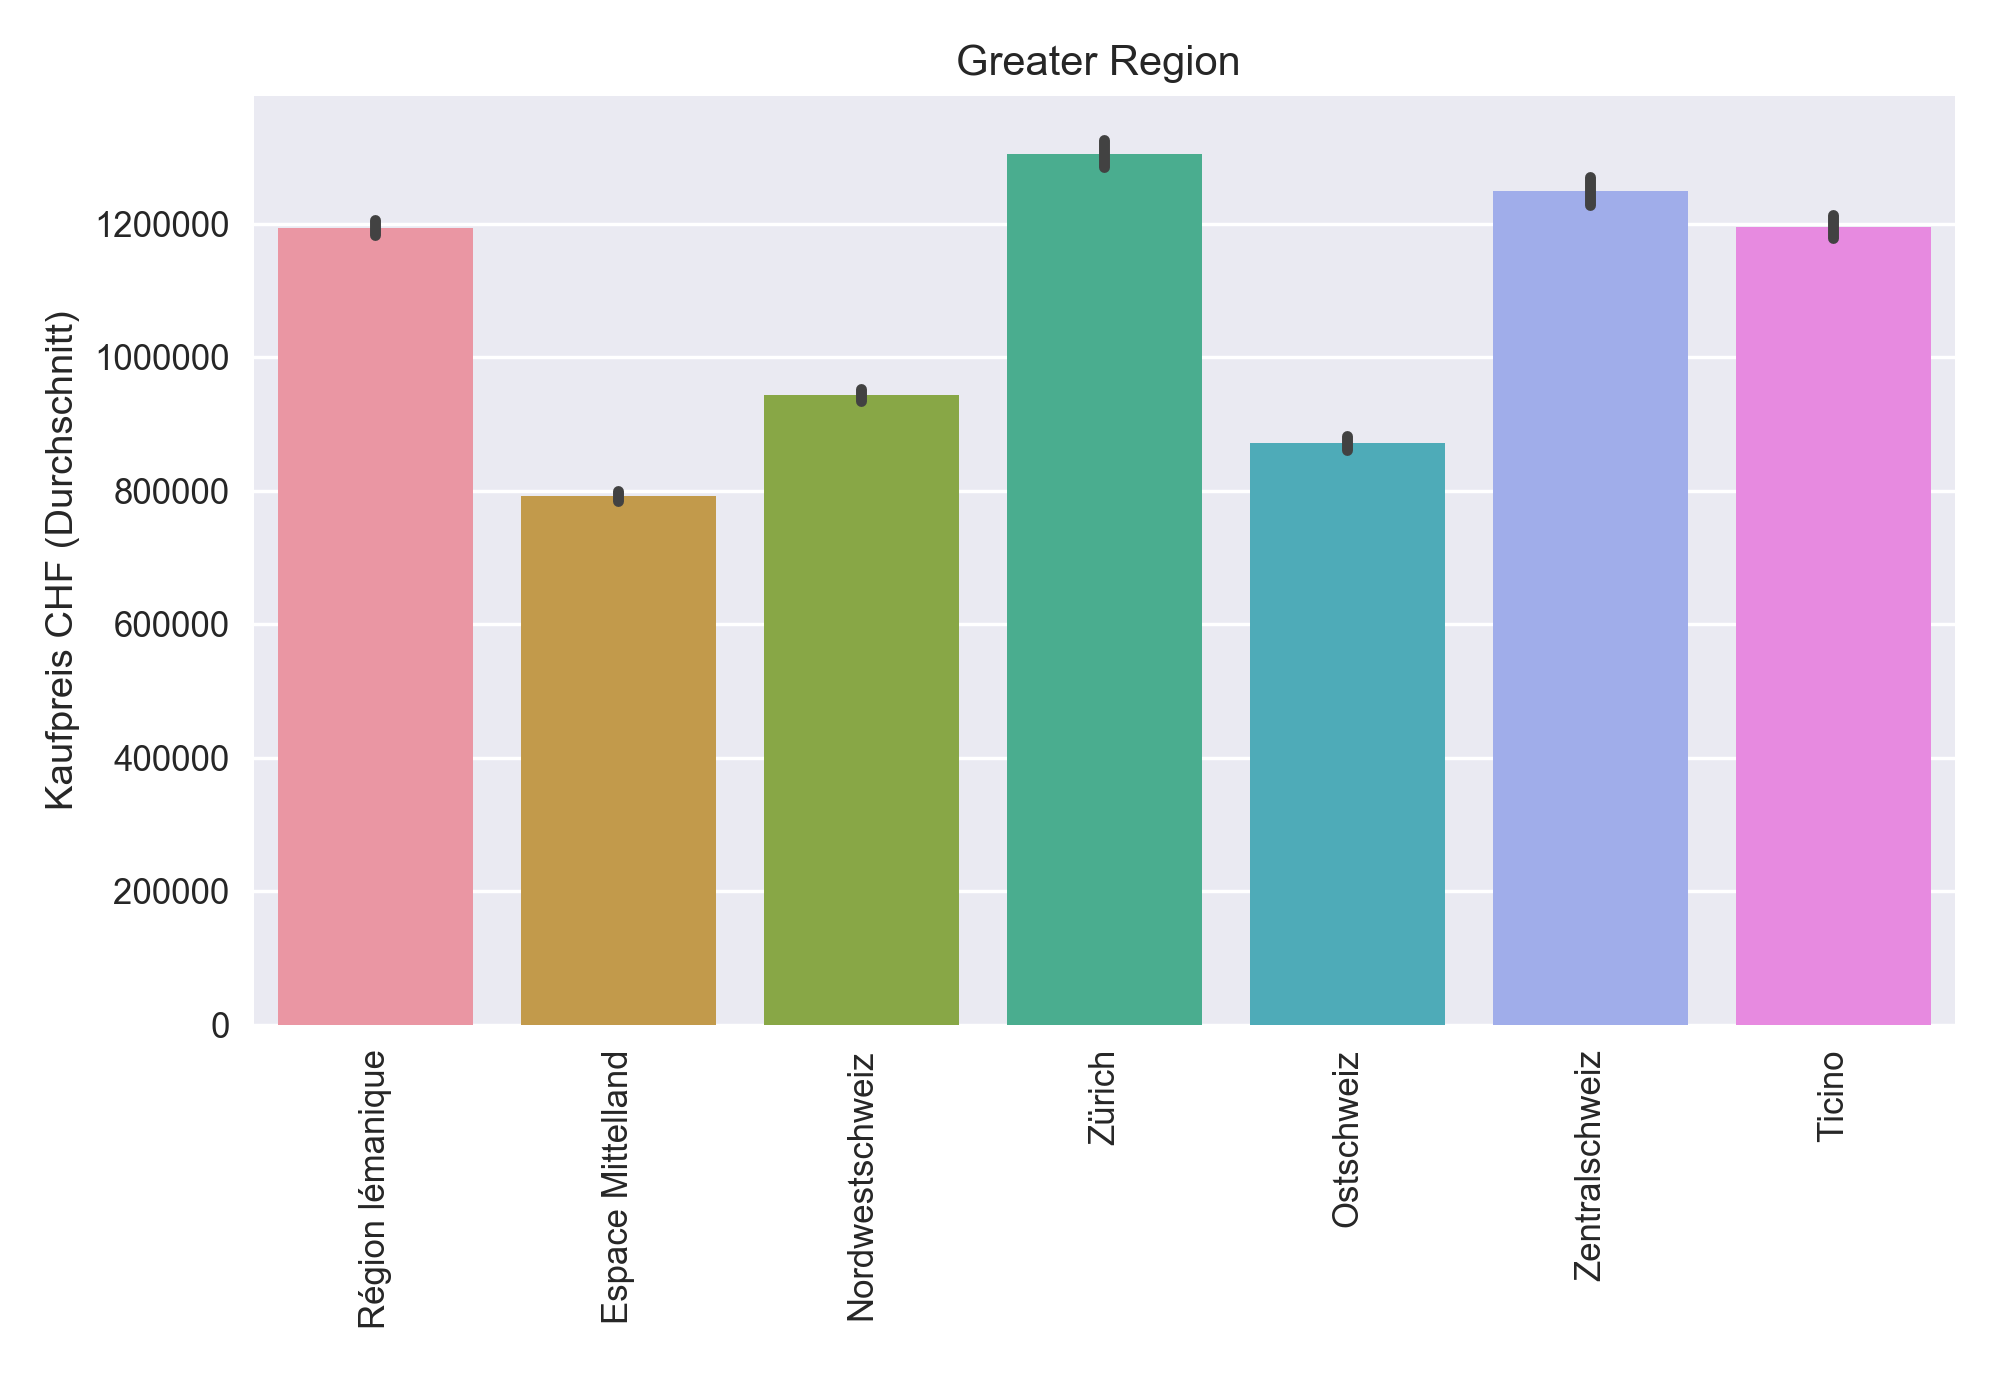
\includegraphics[width=\linewidth]{images/anhang/analysis/barplot_greater_region_id.png}
  \caption{Grossregionen} 
\end{subfigure}
\begin{subfigure}{.5\textwidth}
  \centering
  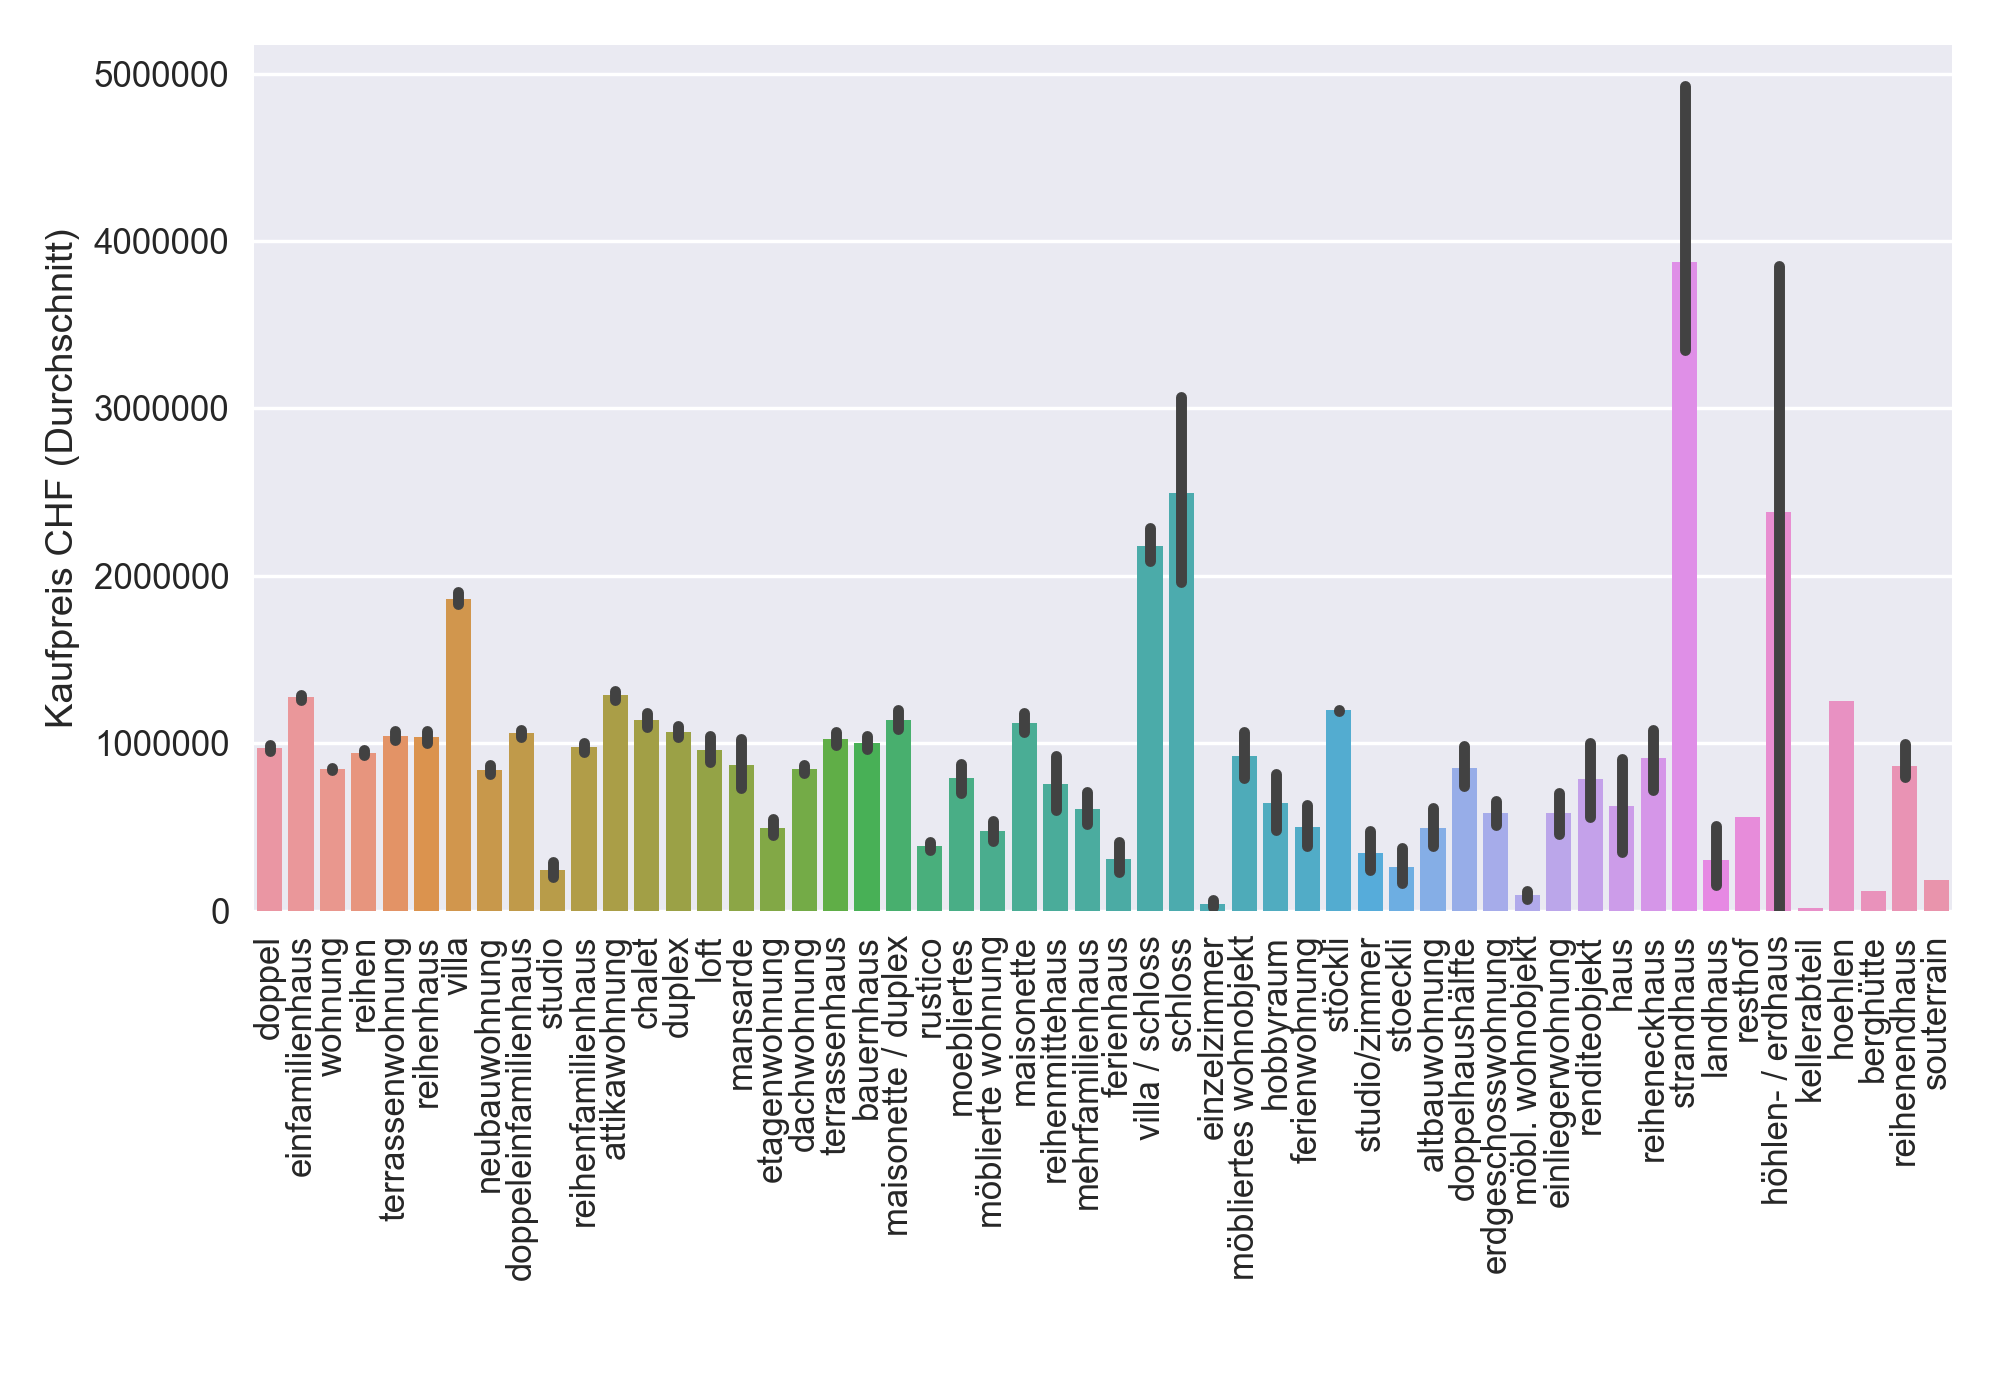
\includegraphics[width=\linewidth]{images/anhang/analysis/barplot_gruppen.png}
  \caption{Immobilientypen} 
\end{subfigure}
\begin{subfigure}{.5\textwidth}
  \centering
  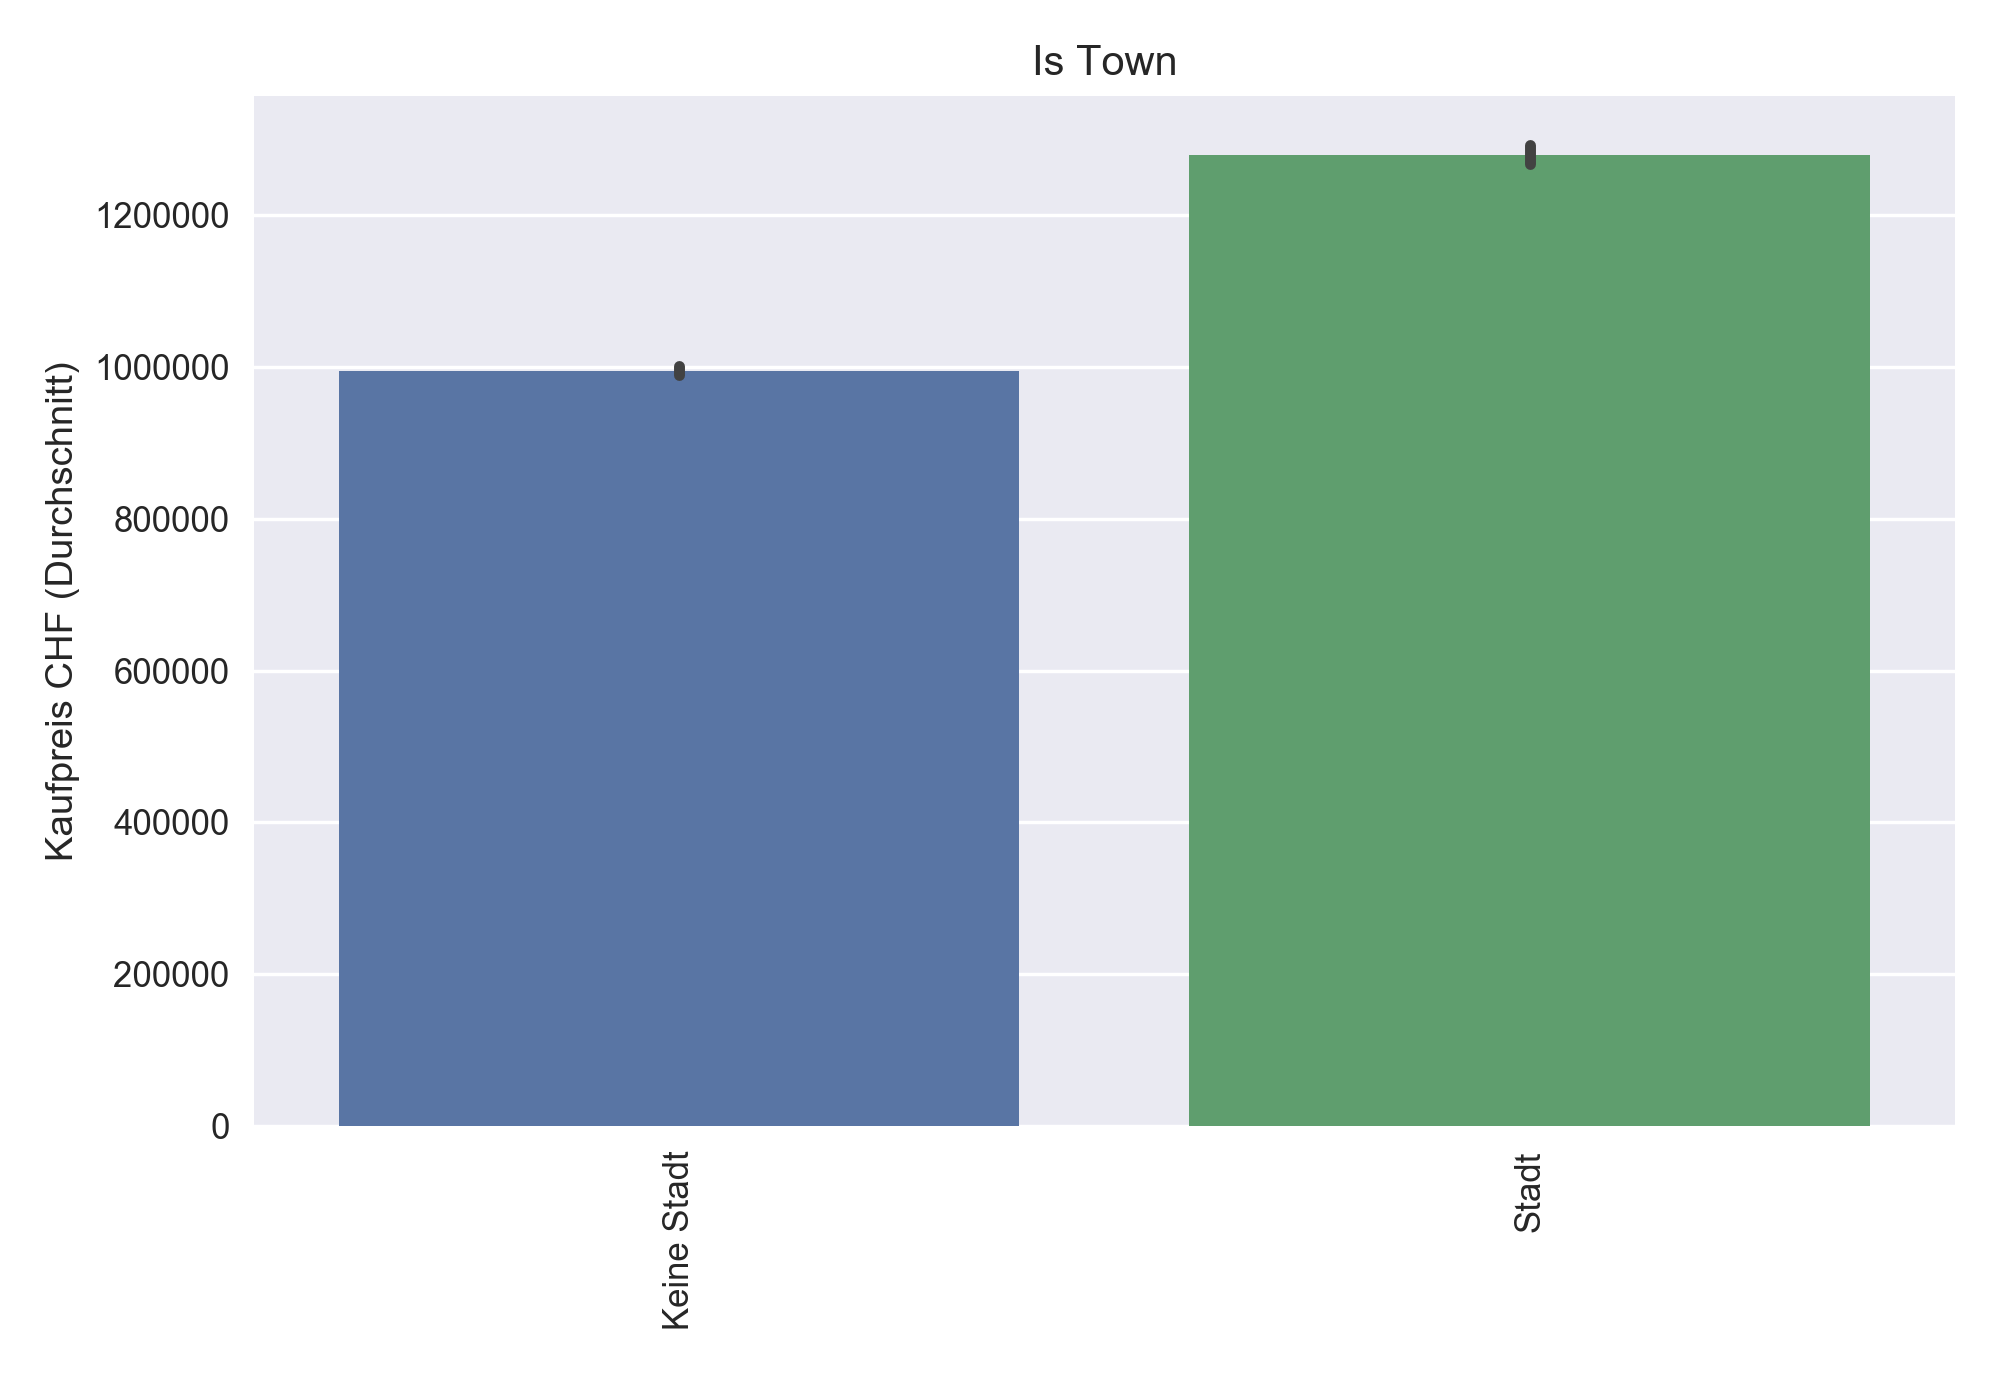
\includegraphics[width=\linewidth]{images/anhang/analysis/barplot_is_town.png}
  \caption{Ist eine Stadt} 
\end{subfigure}
\begin{subfigure}{.5\textwidth}
  \centering
  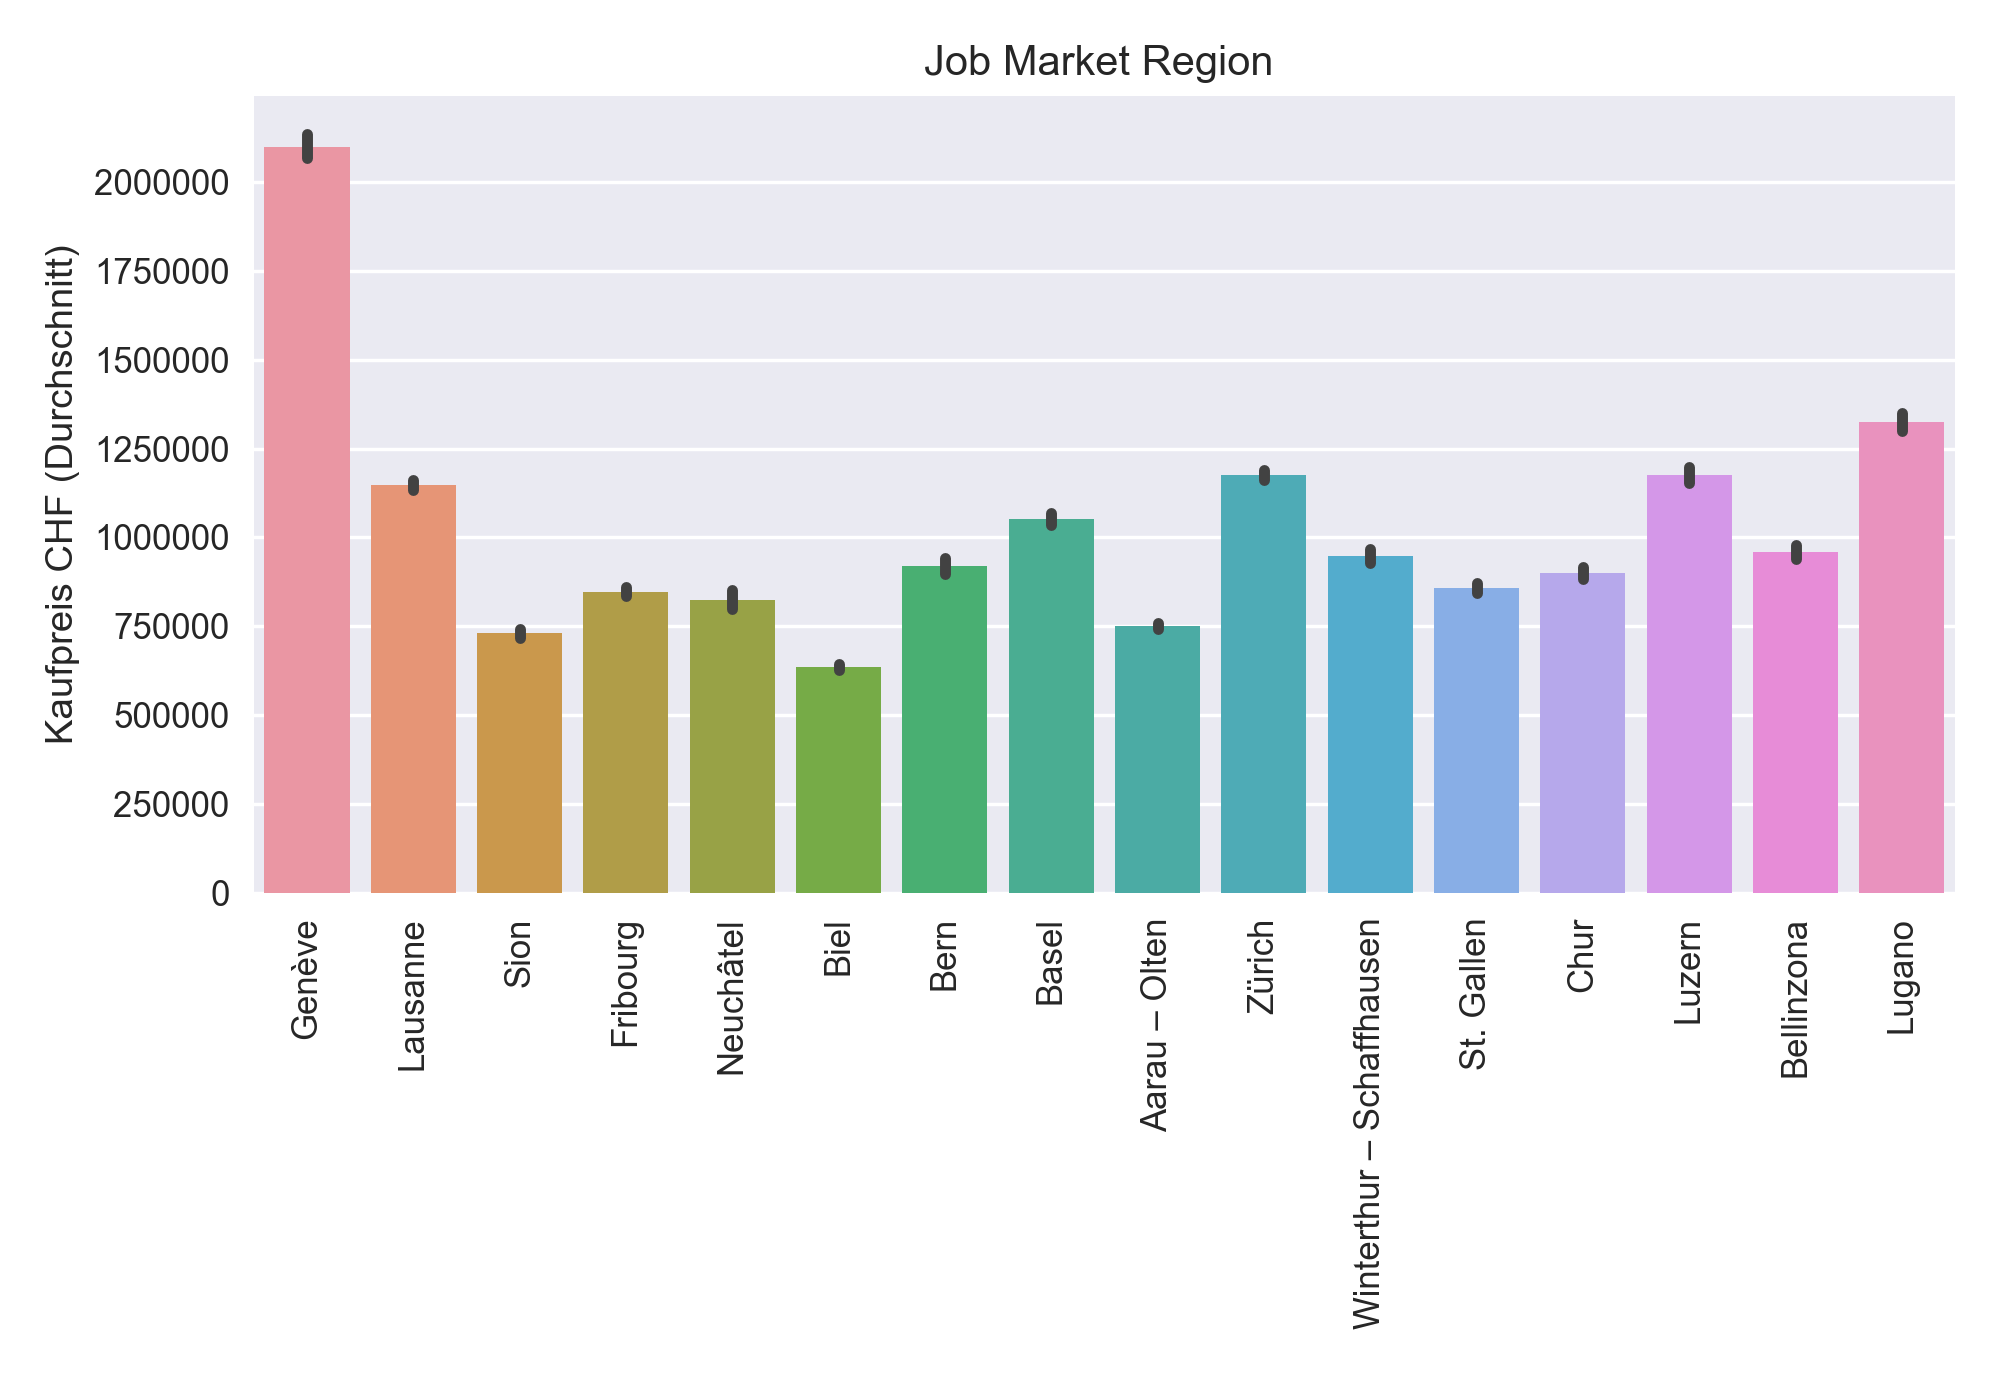
\includegraphics[width=\linewidth]{images/anhang/analysis/barplot_job_market_region_id.png}
  \caption{Jobregionen} 
\end{subfigure}
\begin{subfigure}{.5\textwidth}
  \centering
  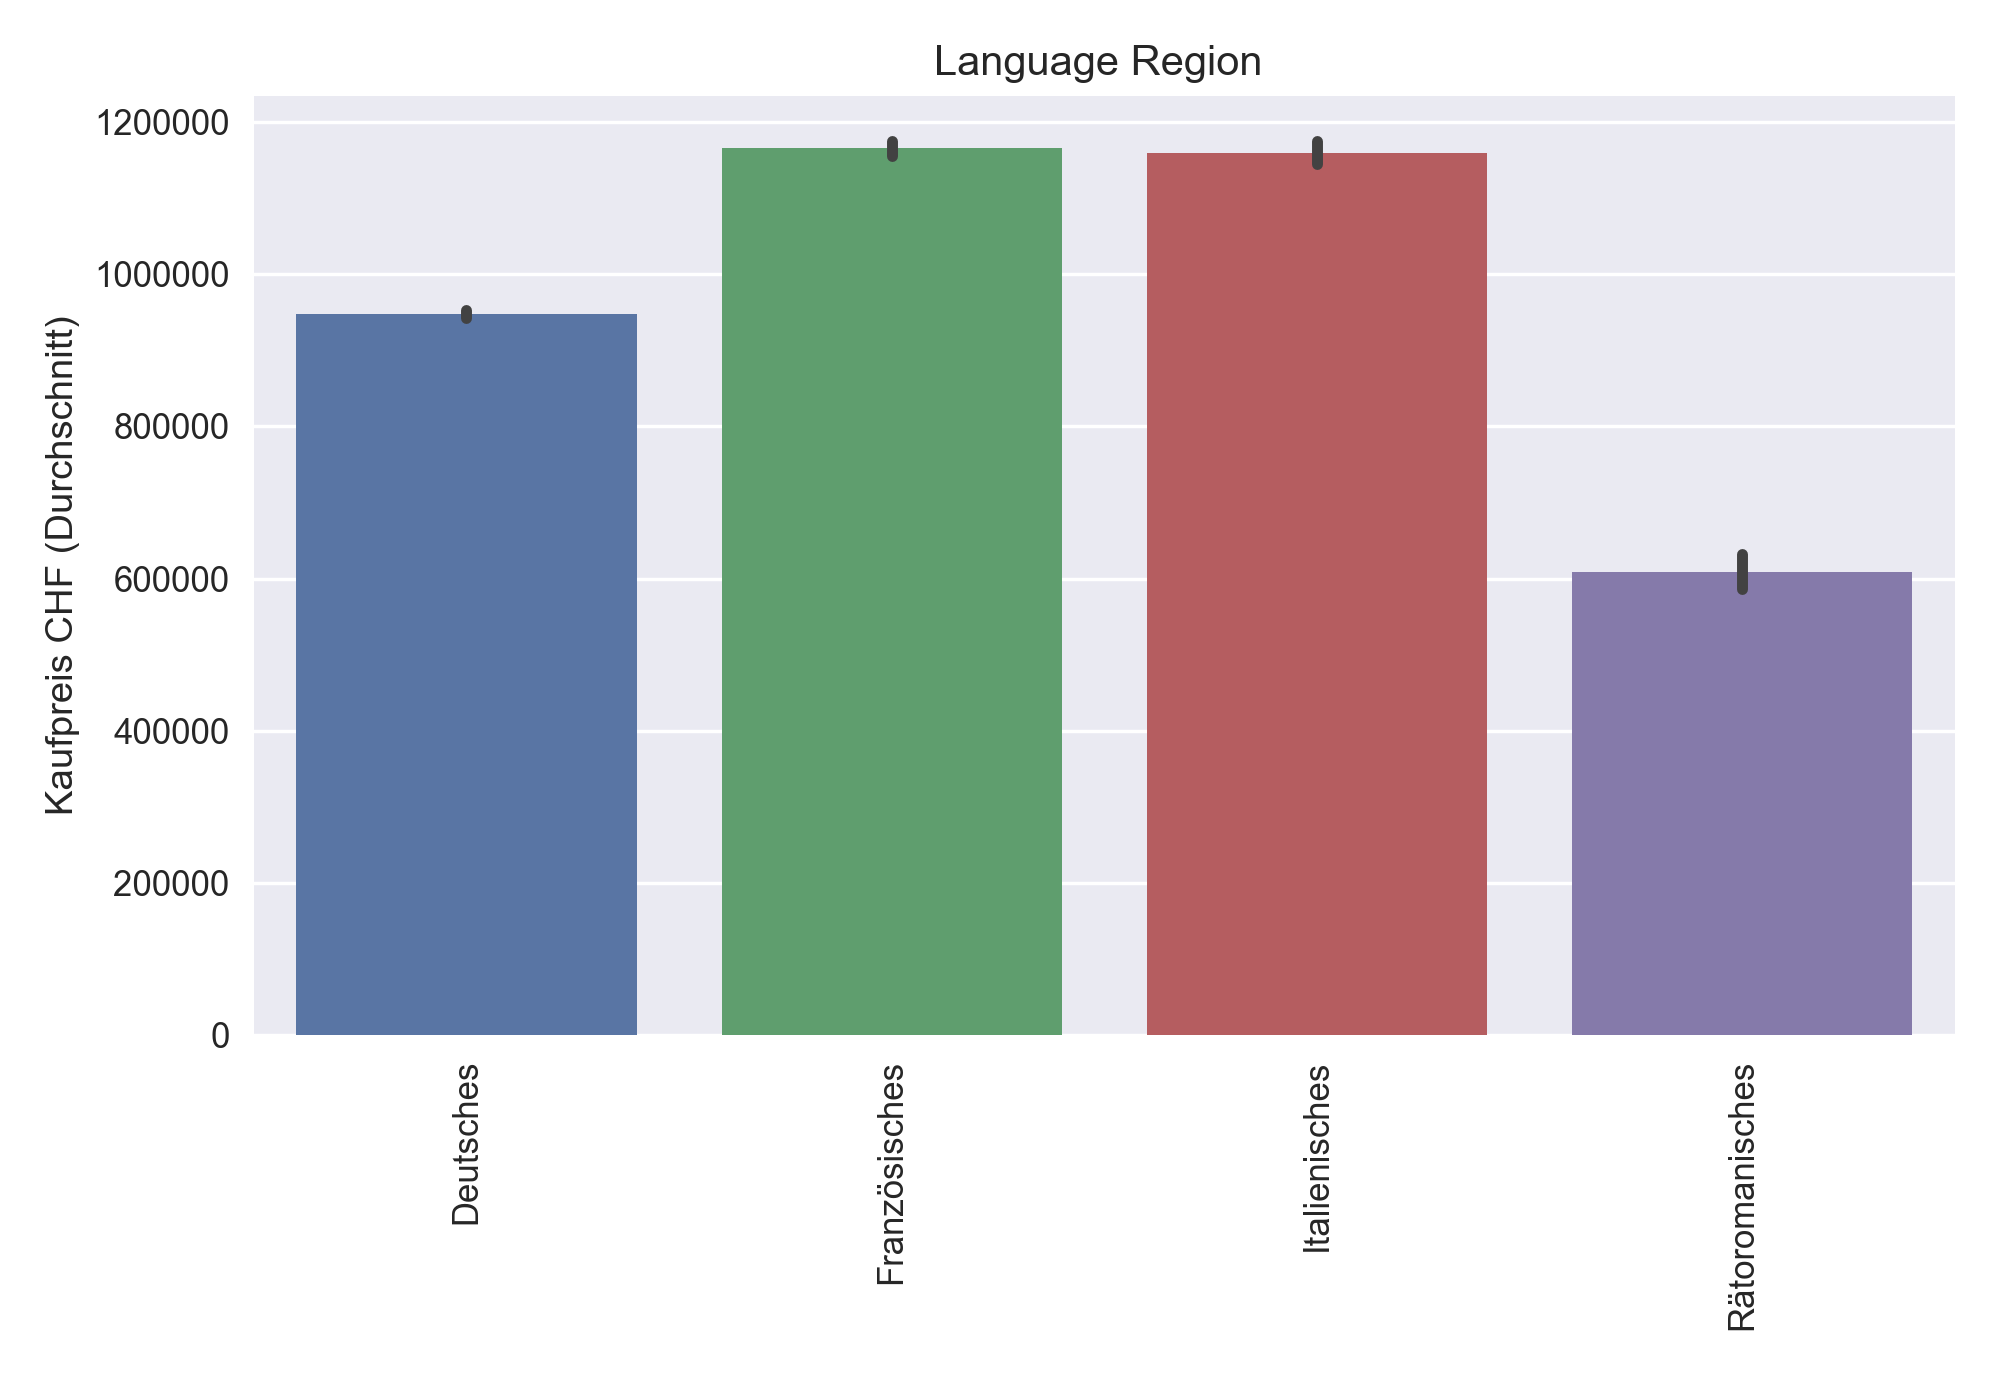
\includegraphics[width=\linewidth]{images/anhang/analysis/barplot_language_region_id.png}
  \caption{Sprachregionen} 
\end{subfigure}
\caption{Barplots für ortsbezogene Kategorien 1}
\end{figure}

\begin{figure}[h]
\begin{subfigure}{.5\textwidth}
  \centering
  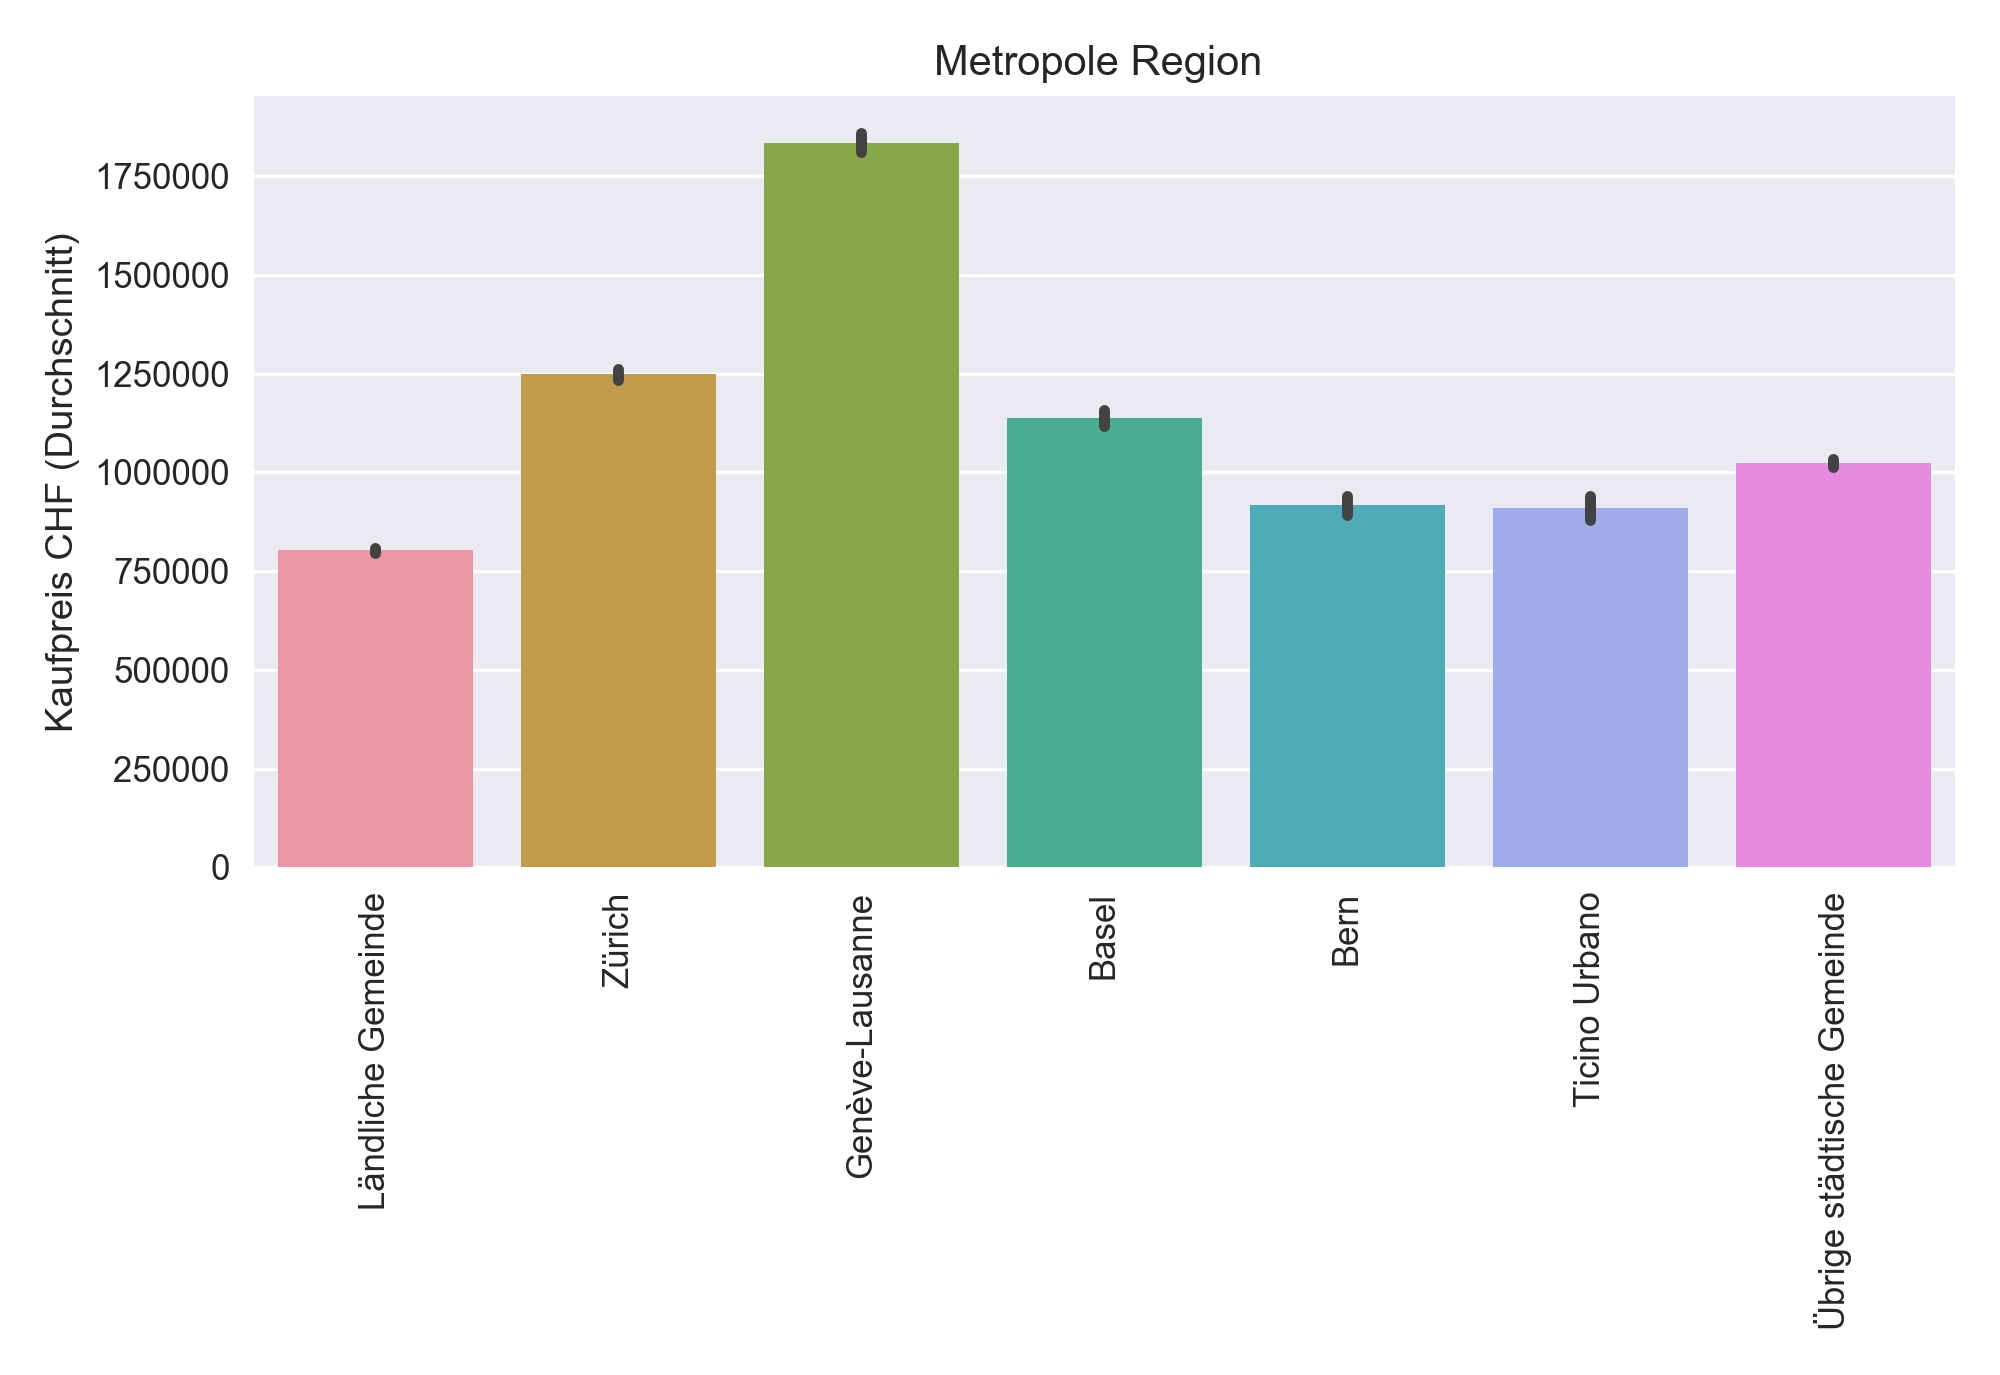
\includegraphics[width=\linewidth]{images/anhang/analysis/barplot_metropole_region_id.png}
  \caption{Metropolregionen}
\end{subfigure}
\begin{subfigure}{.5\textwidth}
  \centering
  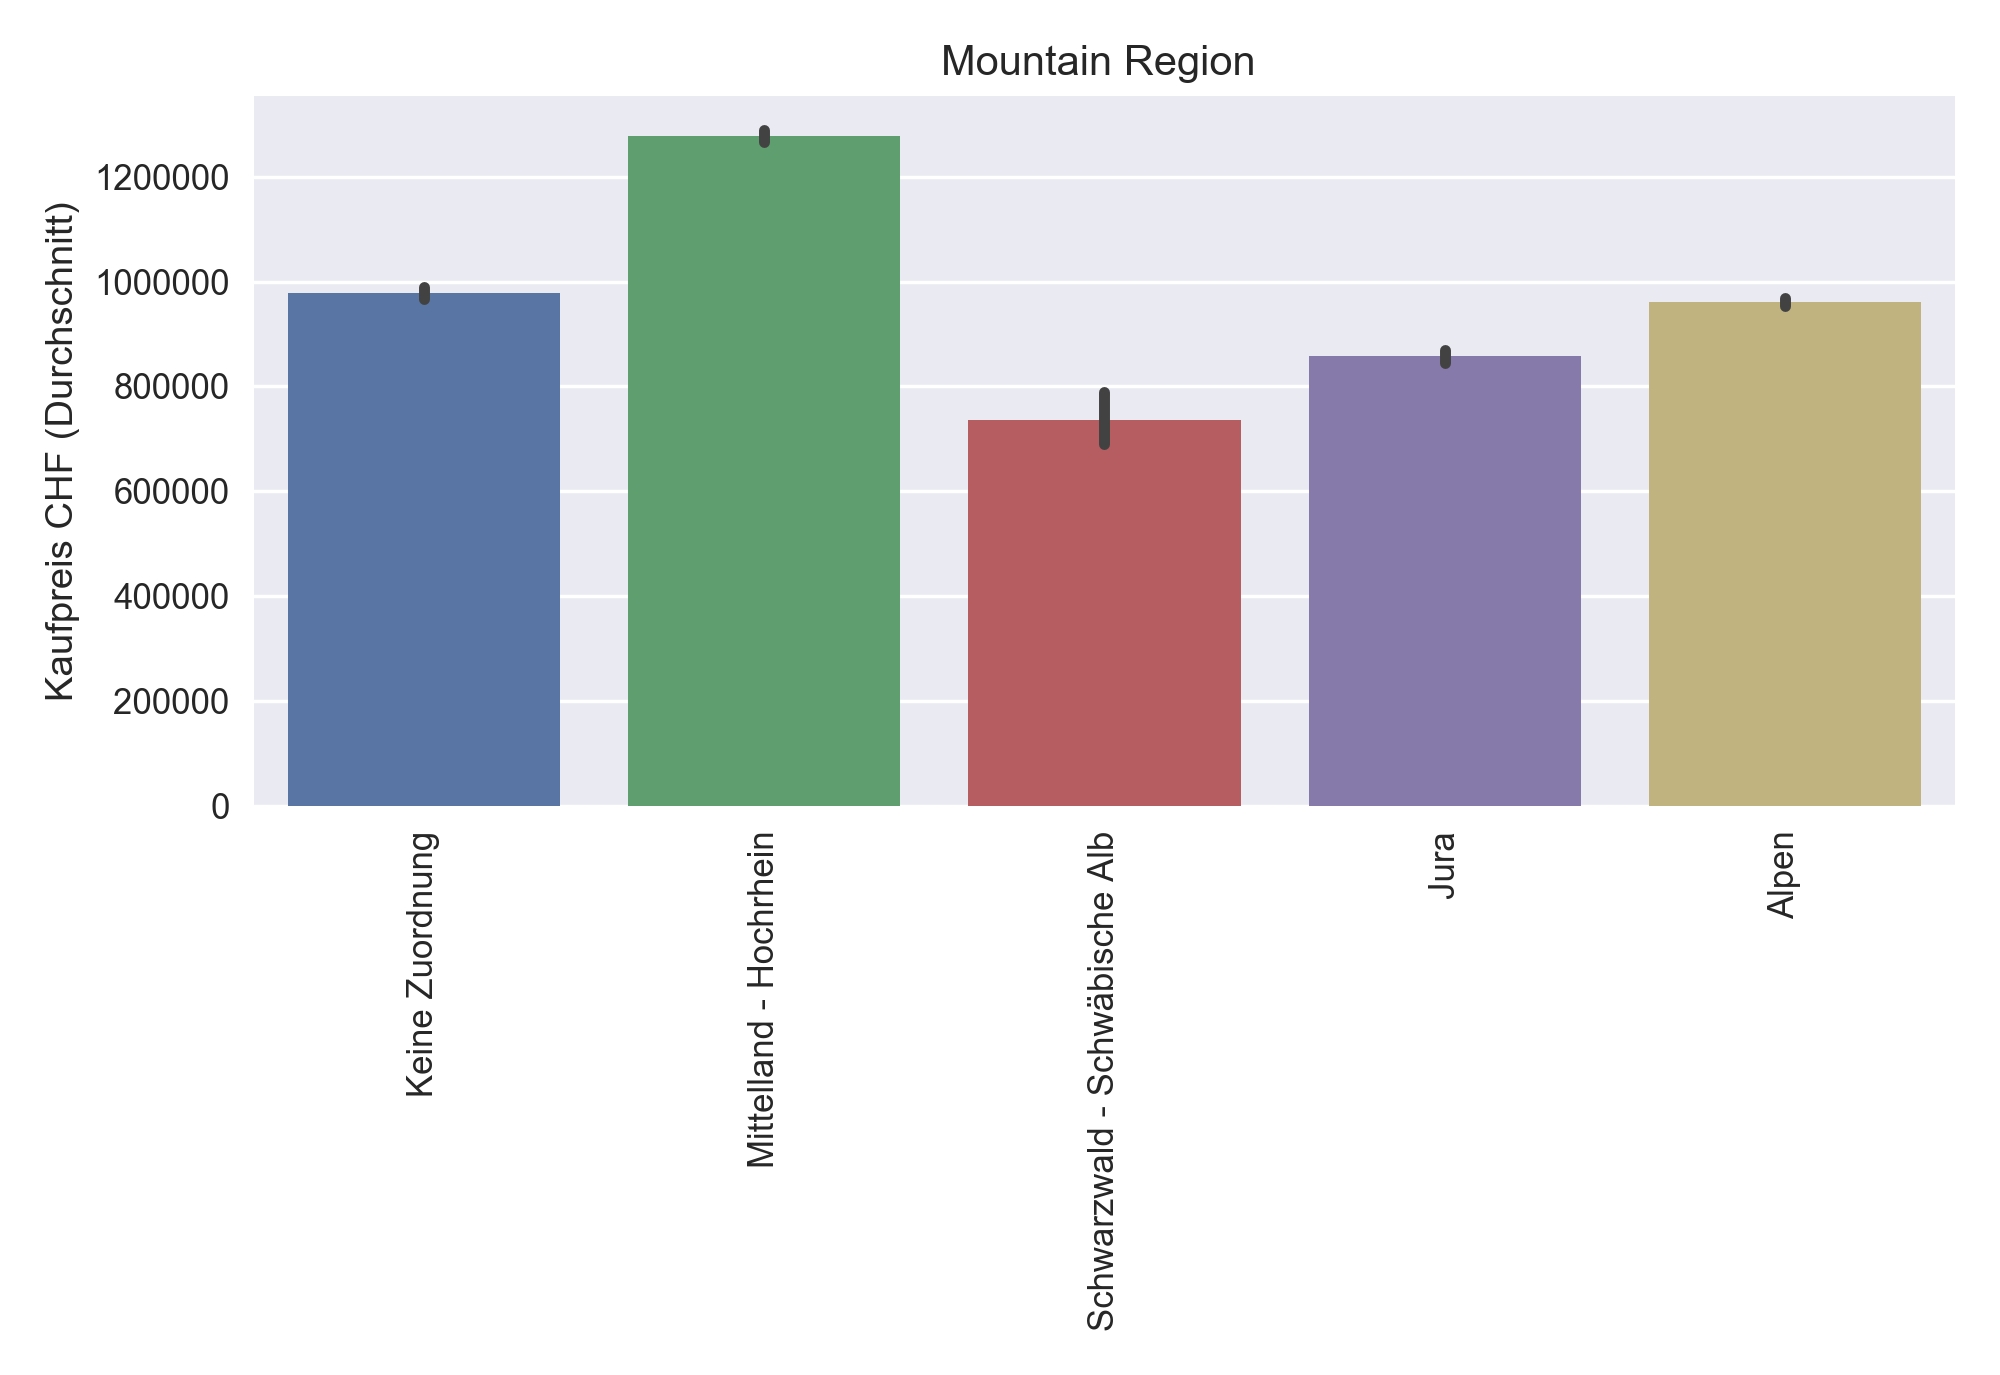
\includegraphics[width=\linewidth]{images/anhang/analysis/barplot_mountain_region_id.png}
  \caption{Bergregionen} 
\end{subfigure}
\begin{subfigure}{.5\textwidth}
  \centering
  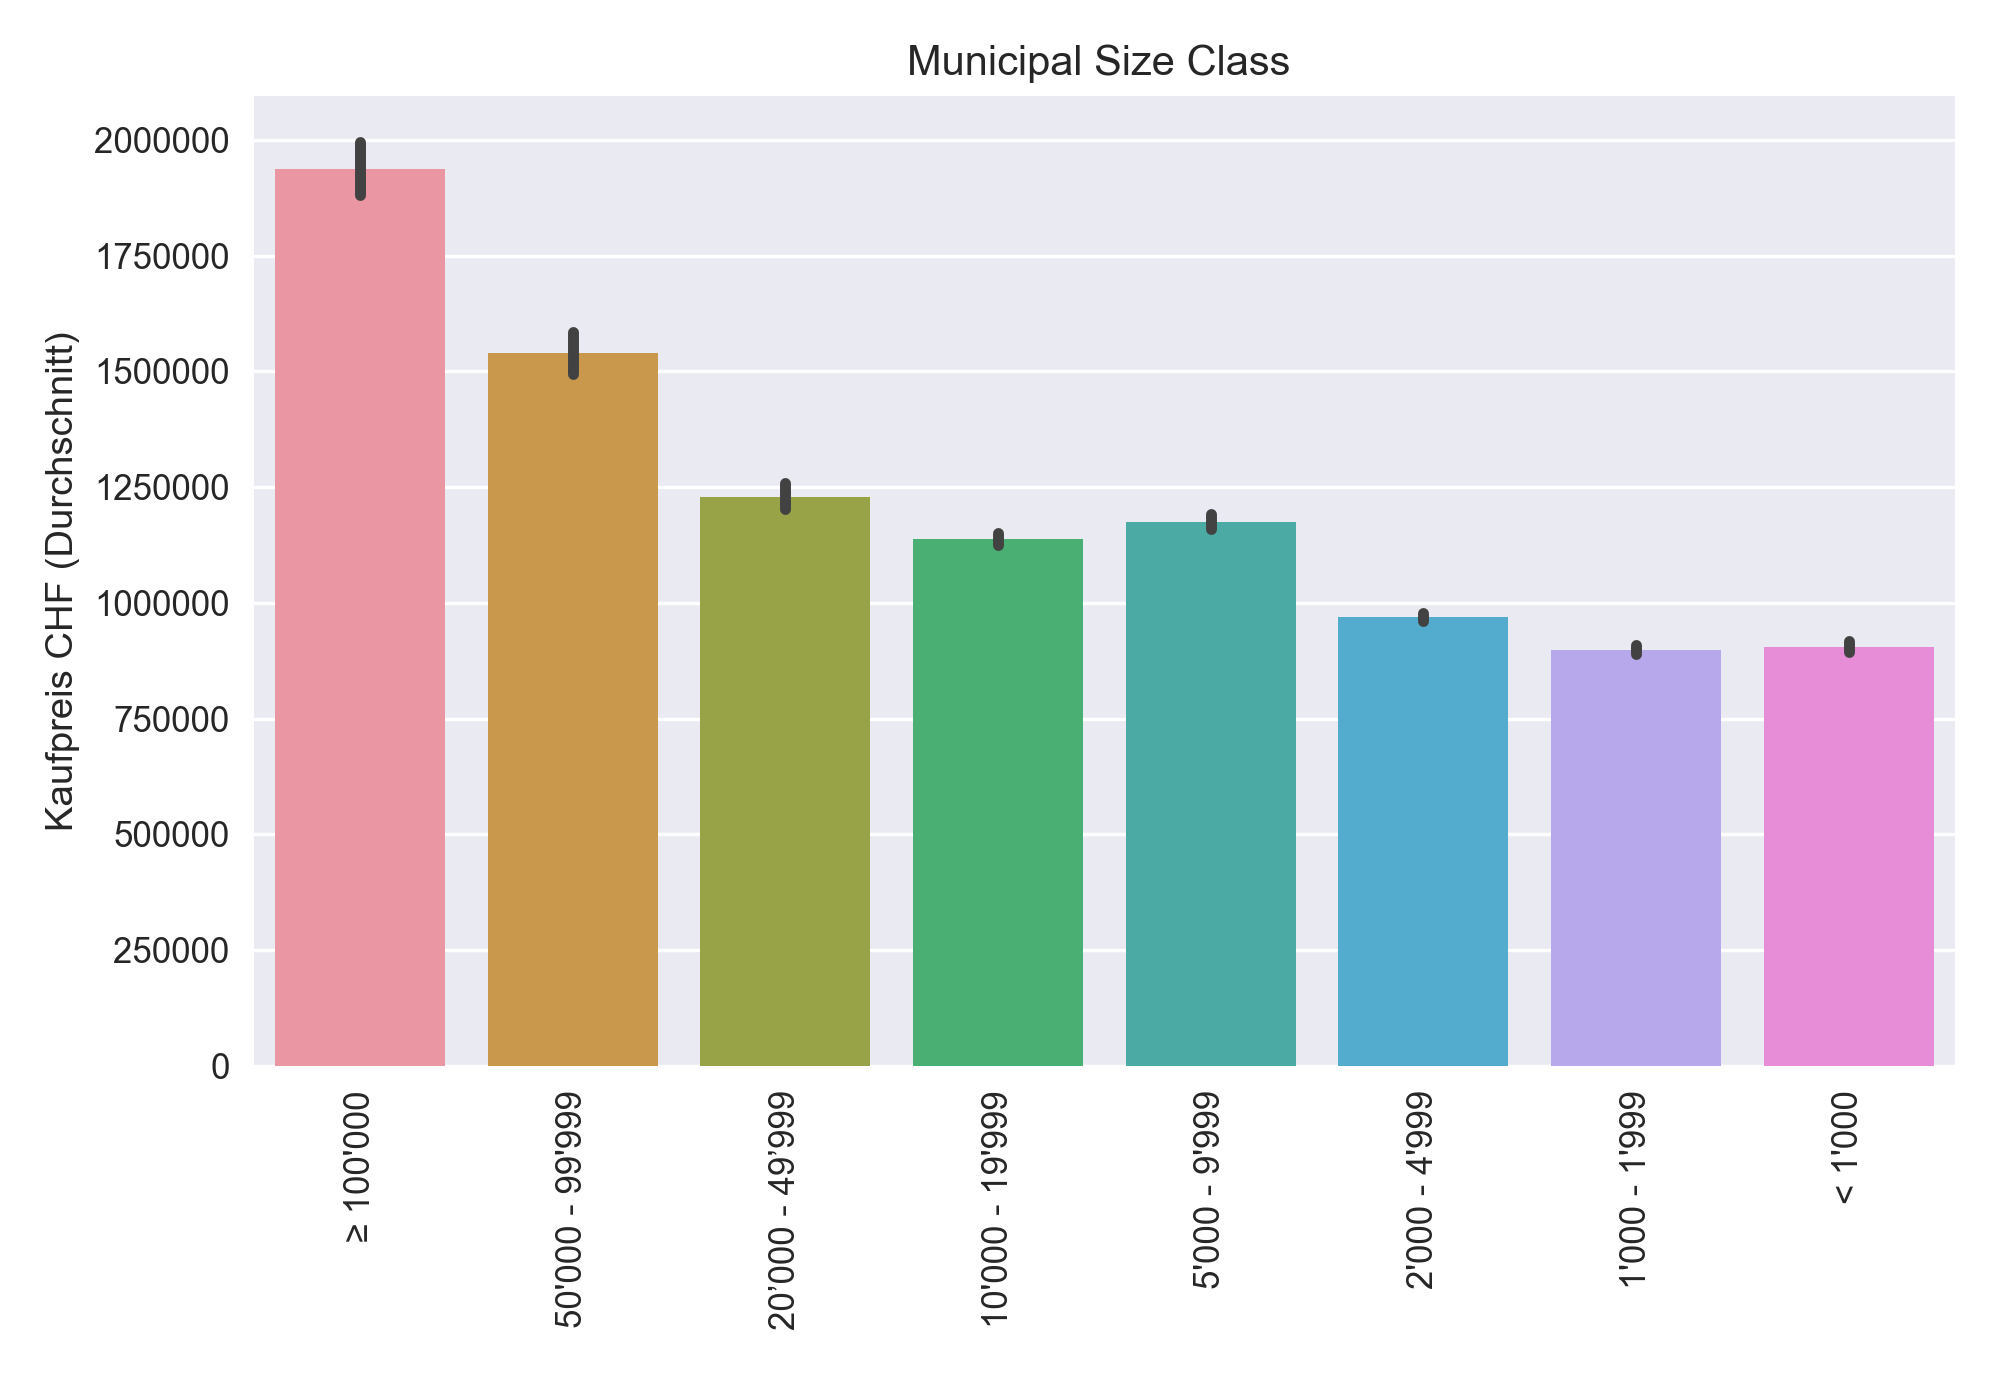
\includegraphics[width=\linewidth]{images/anhang/analysis/barplot_municipal_size_class_id.png}
  \caption{Gemeindegrössen}
\end{subfigure}
\begin{subfigure}{.5\textwidth}
  \centering
  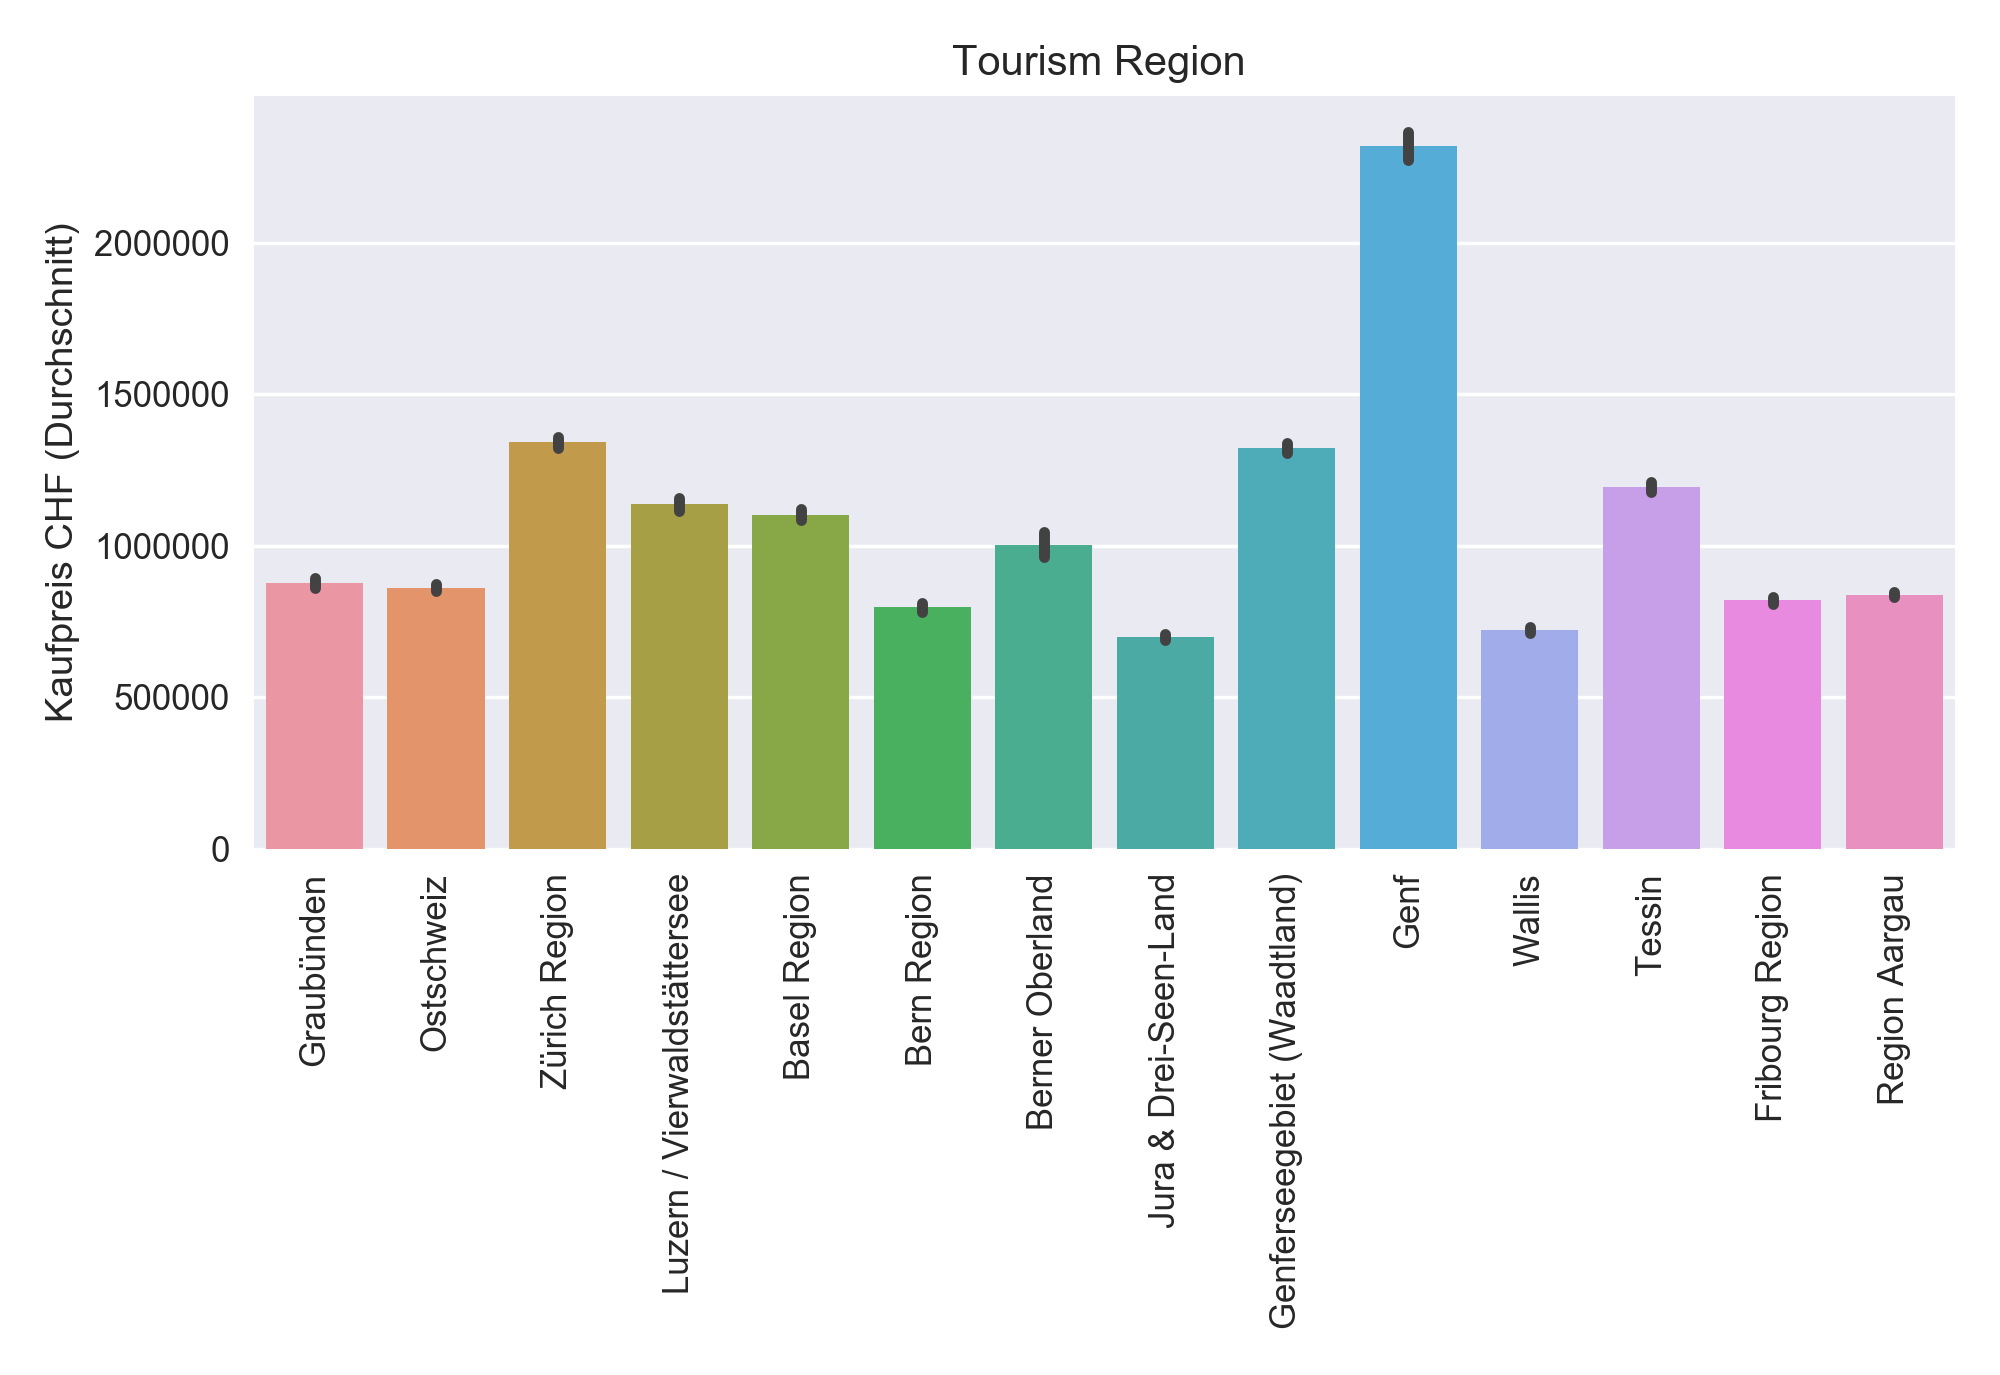
\includegraphics[width=\linewidth]{images/anhang/analysis/barplot_tourism_region_id.png}
  \caption{Tourismusregionen} 
\end{subfigure}
\caption{Barplots für ortsbezogene Kategorien 2}
\end{figure}

\begin{figure}[h]
\begin{subfigure}{.5\textwidth}
  \centering
  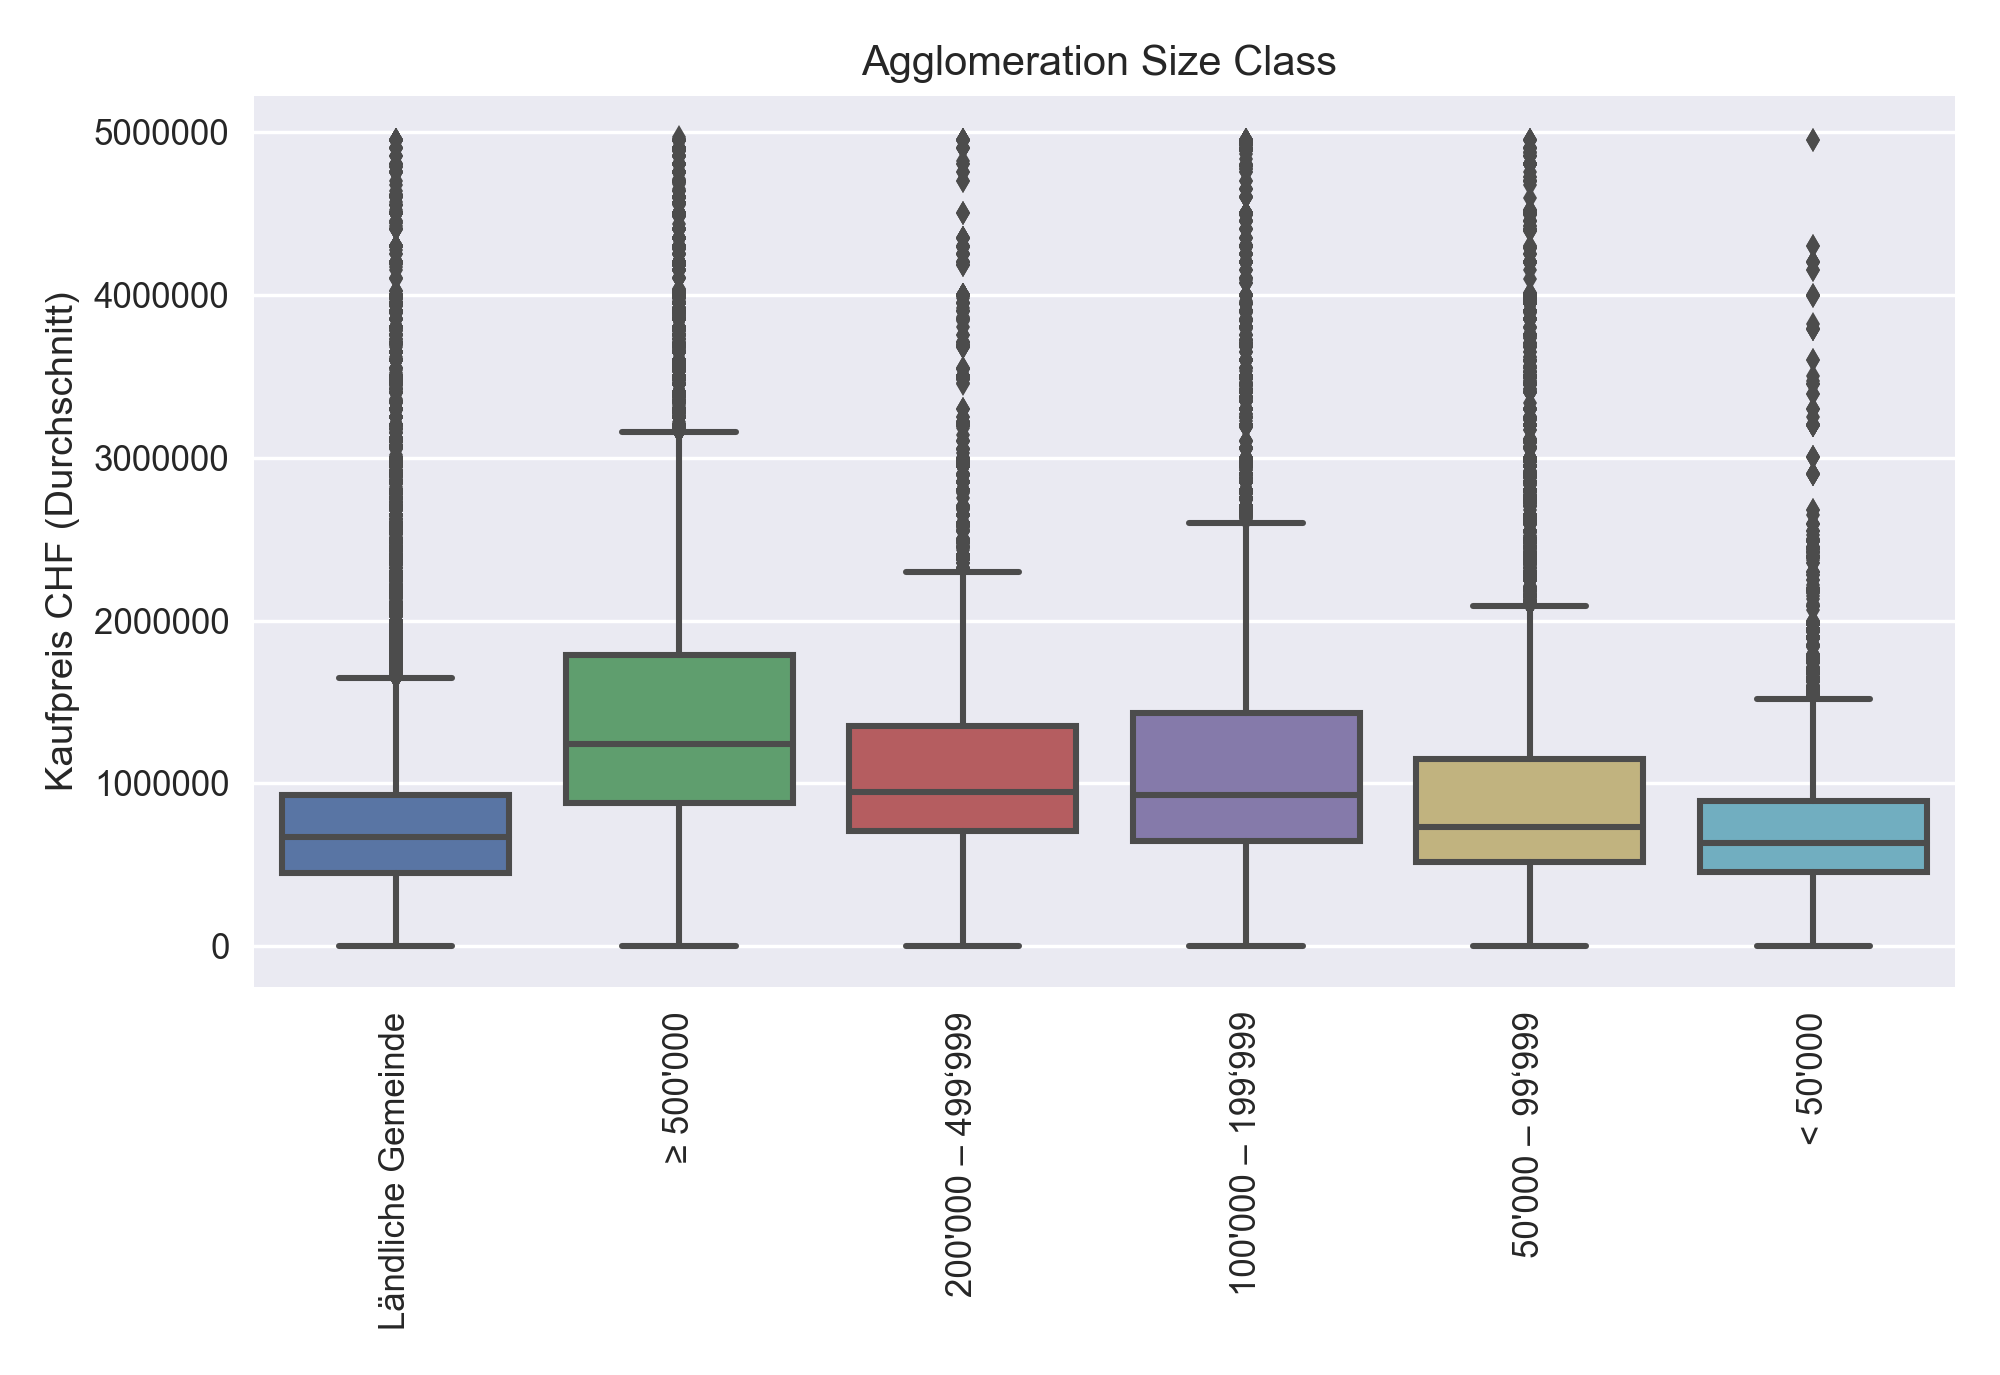
\includegraphics[width=\linewidth]{images/anhang/analysis/boxplot_agglomeration_size_class_id.png}
  \caption{Agglomerationsgrössen}
\end{subfigure}
\begin{subfigure}{.5\textwidth}
  \centering
  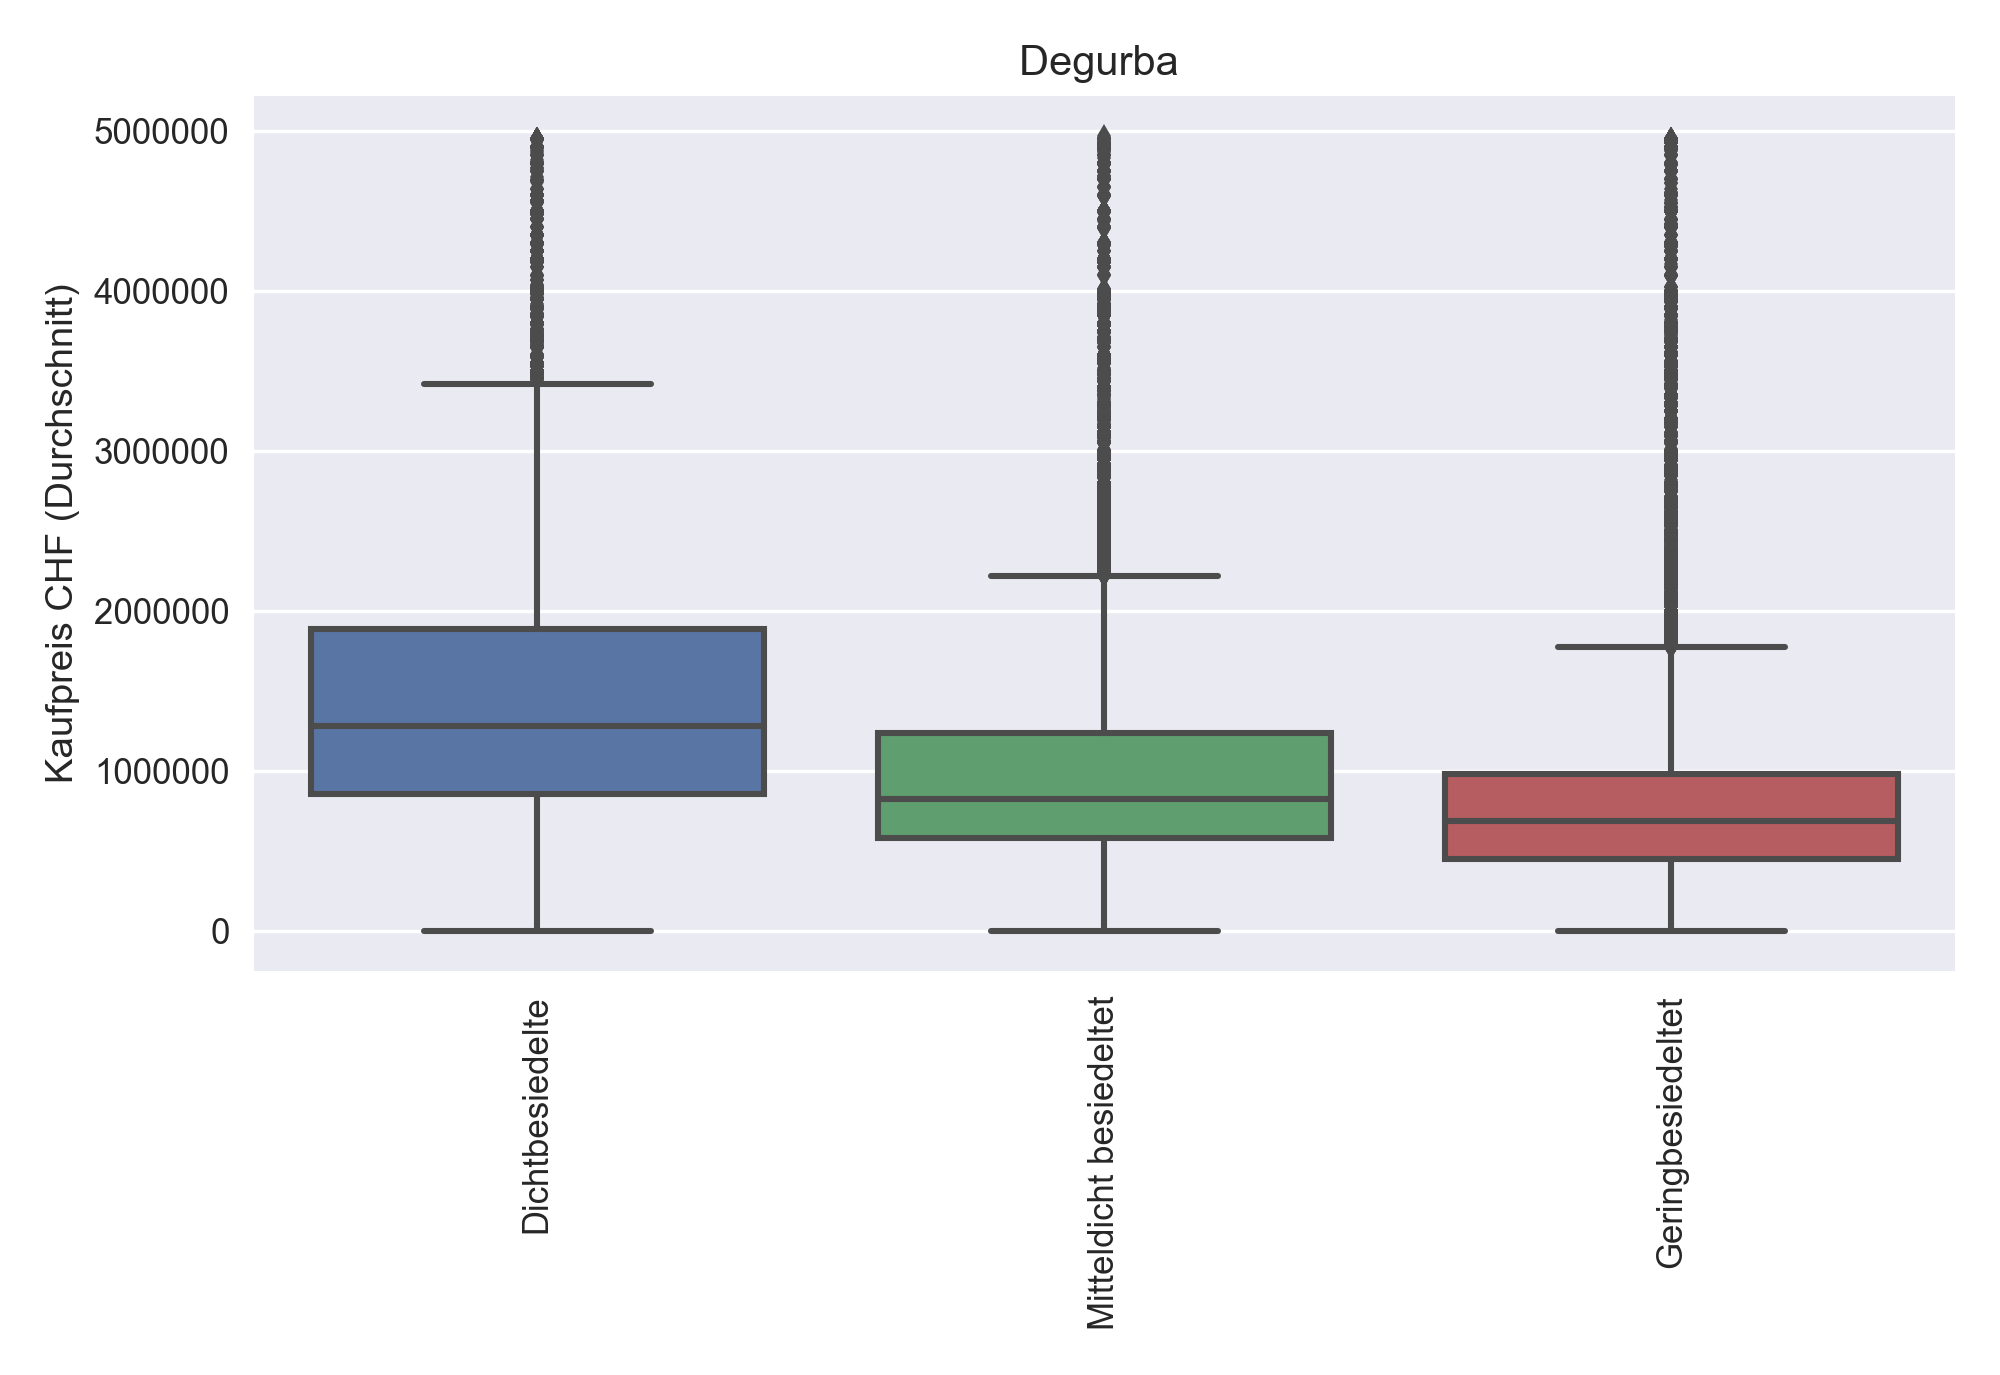
\includegraphics[width=\linewidth]{images/anhang/analysis/boxplot_degurba_id.png}
  \caption{Grad der Urbanisierung} 
\end{subfigure}
\begin{subfigure}{.5\textwidth}
  \centering
  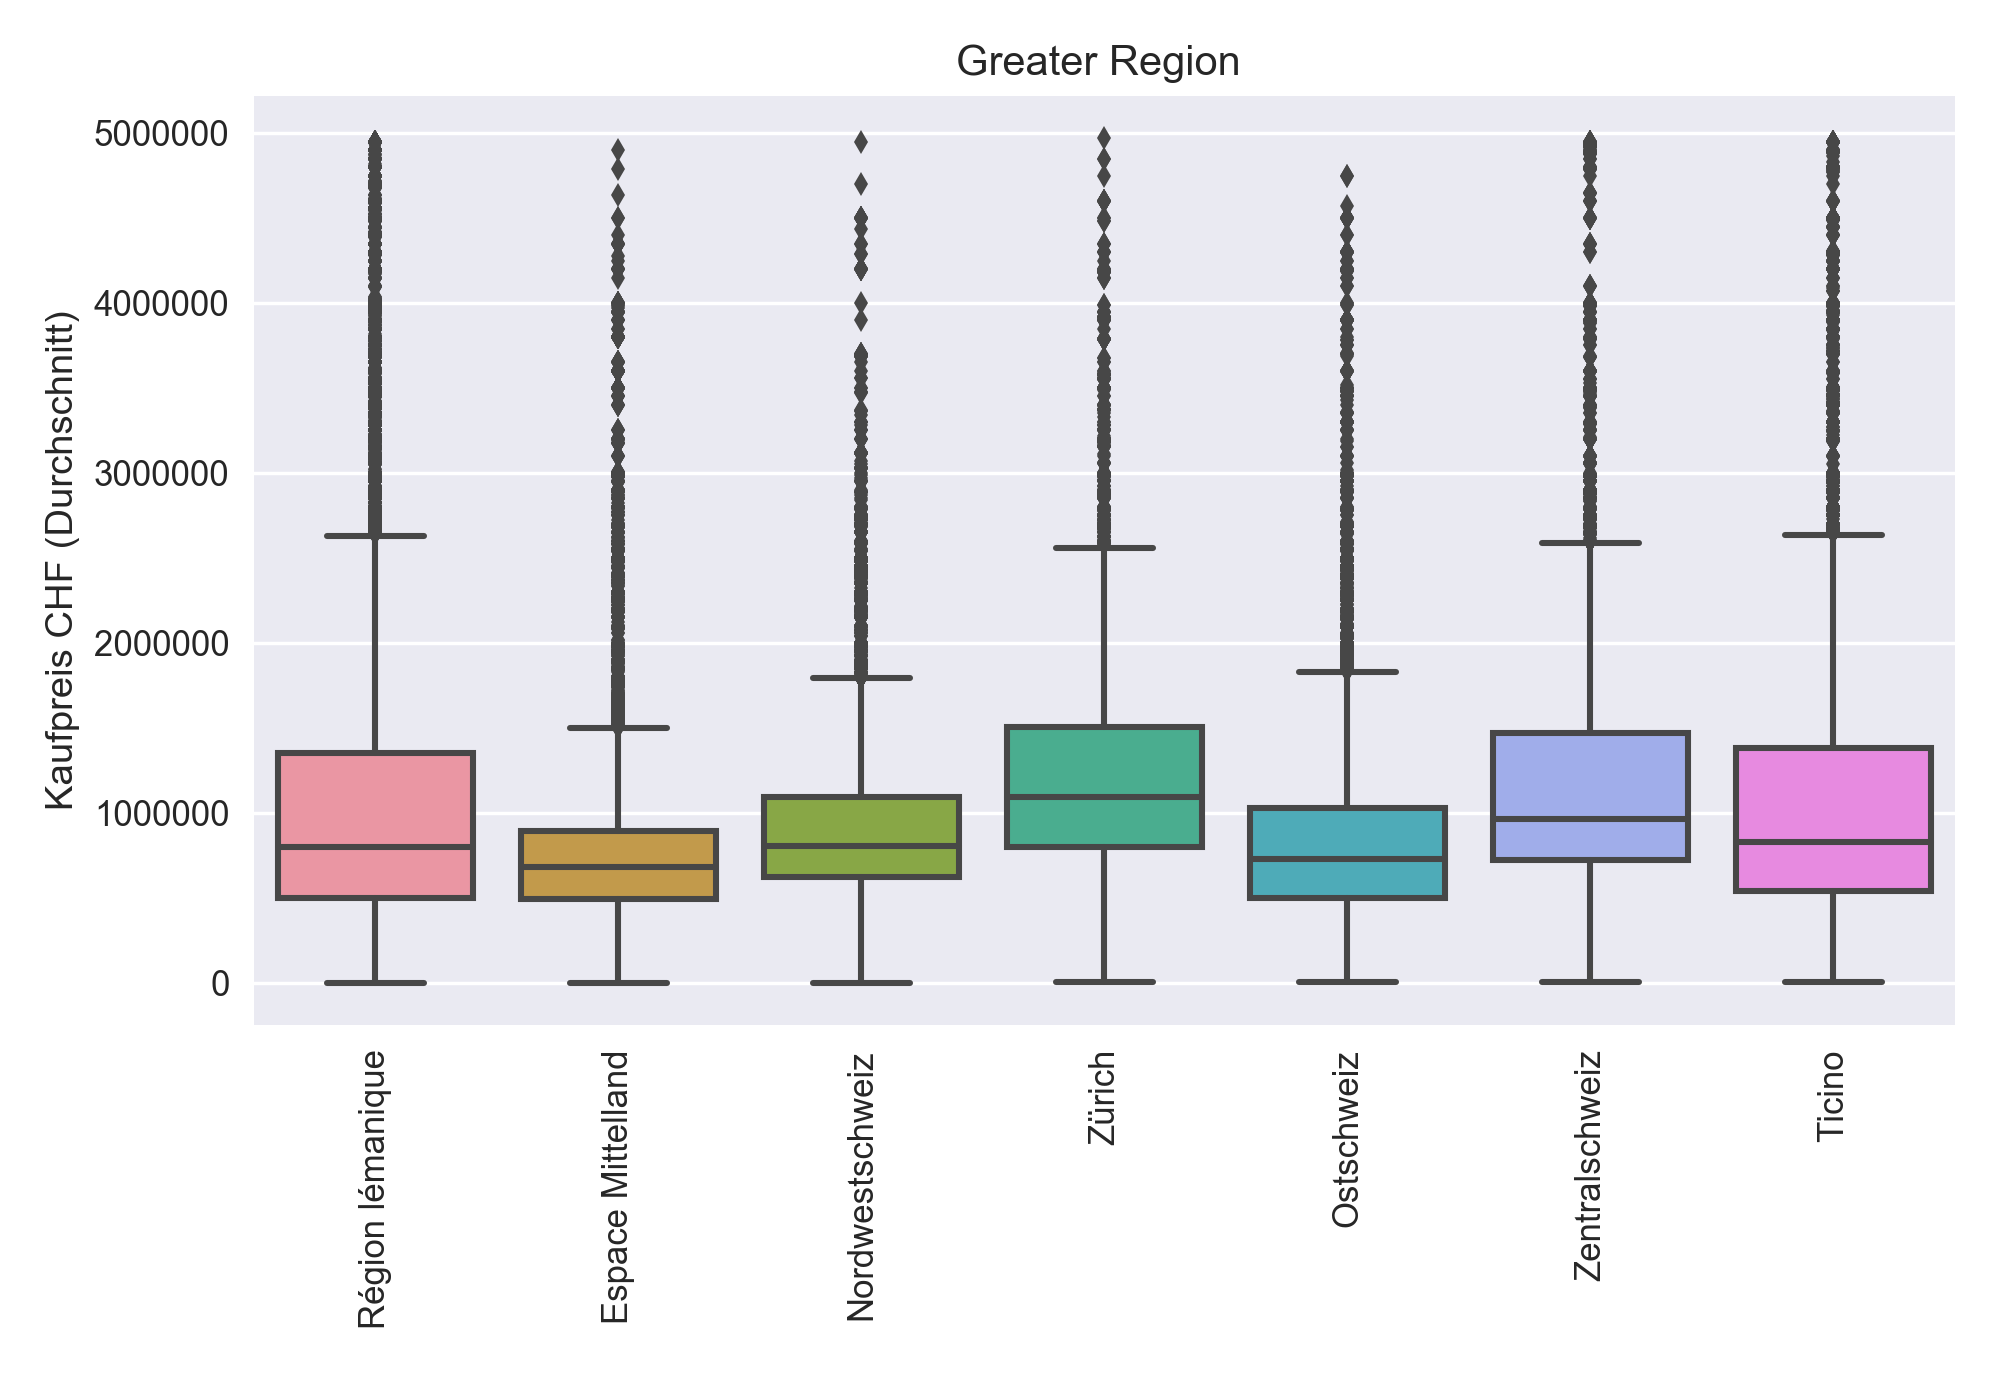
\includegraphics[width=\linewidth]{images/anhang/analysis/boxplot_greater_region_id.png}
  \caption{Grossregionen}
\end{subfigure}
\begin{subfigure}{.5\textwidth}
  \centering
  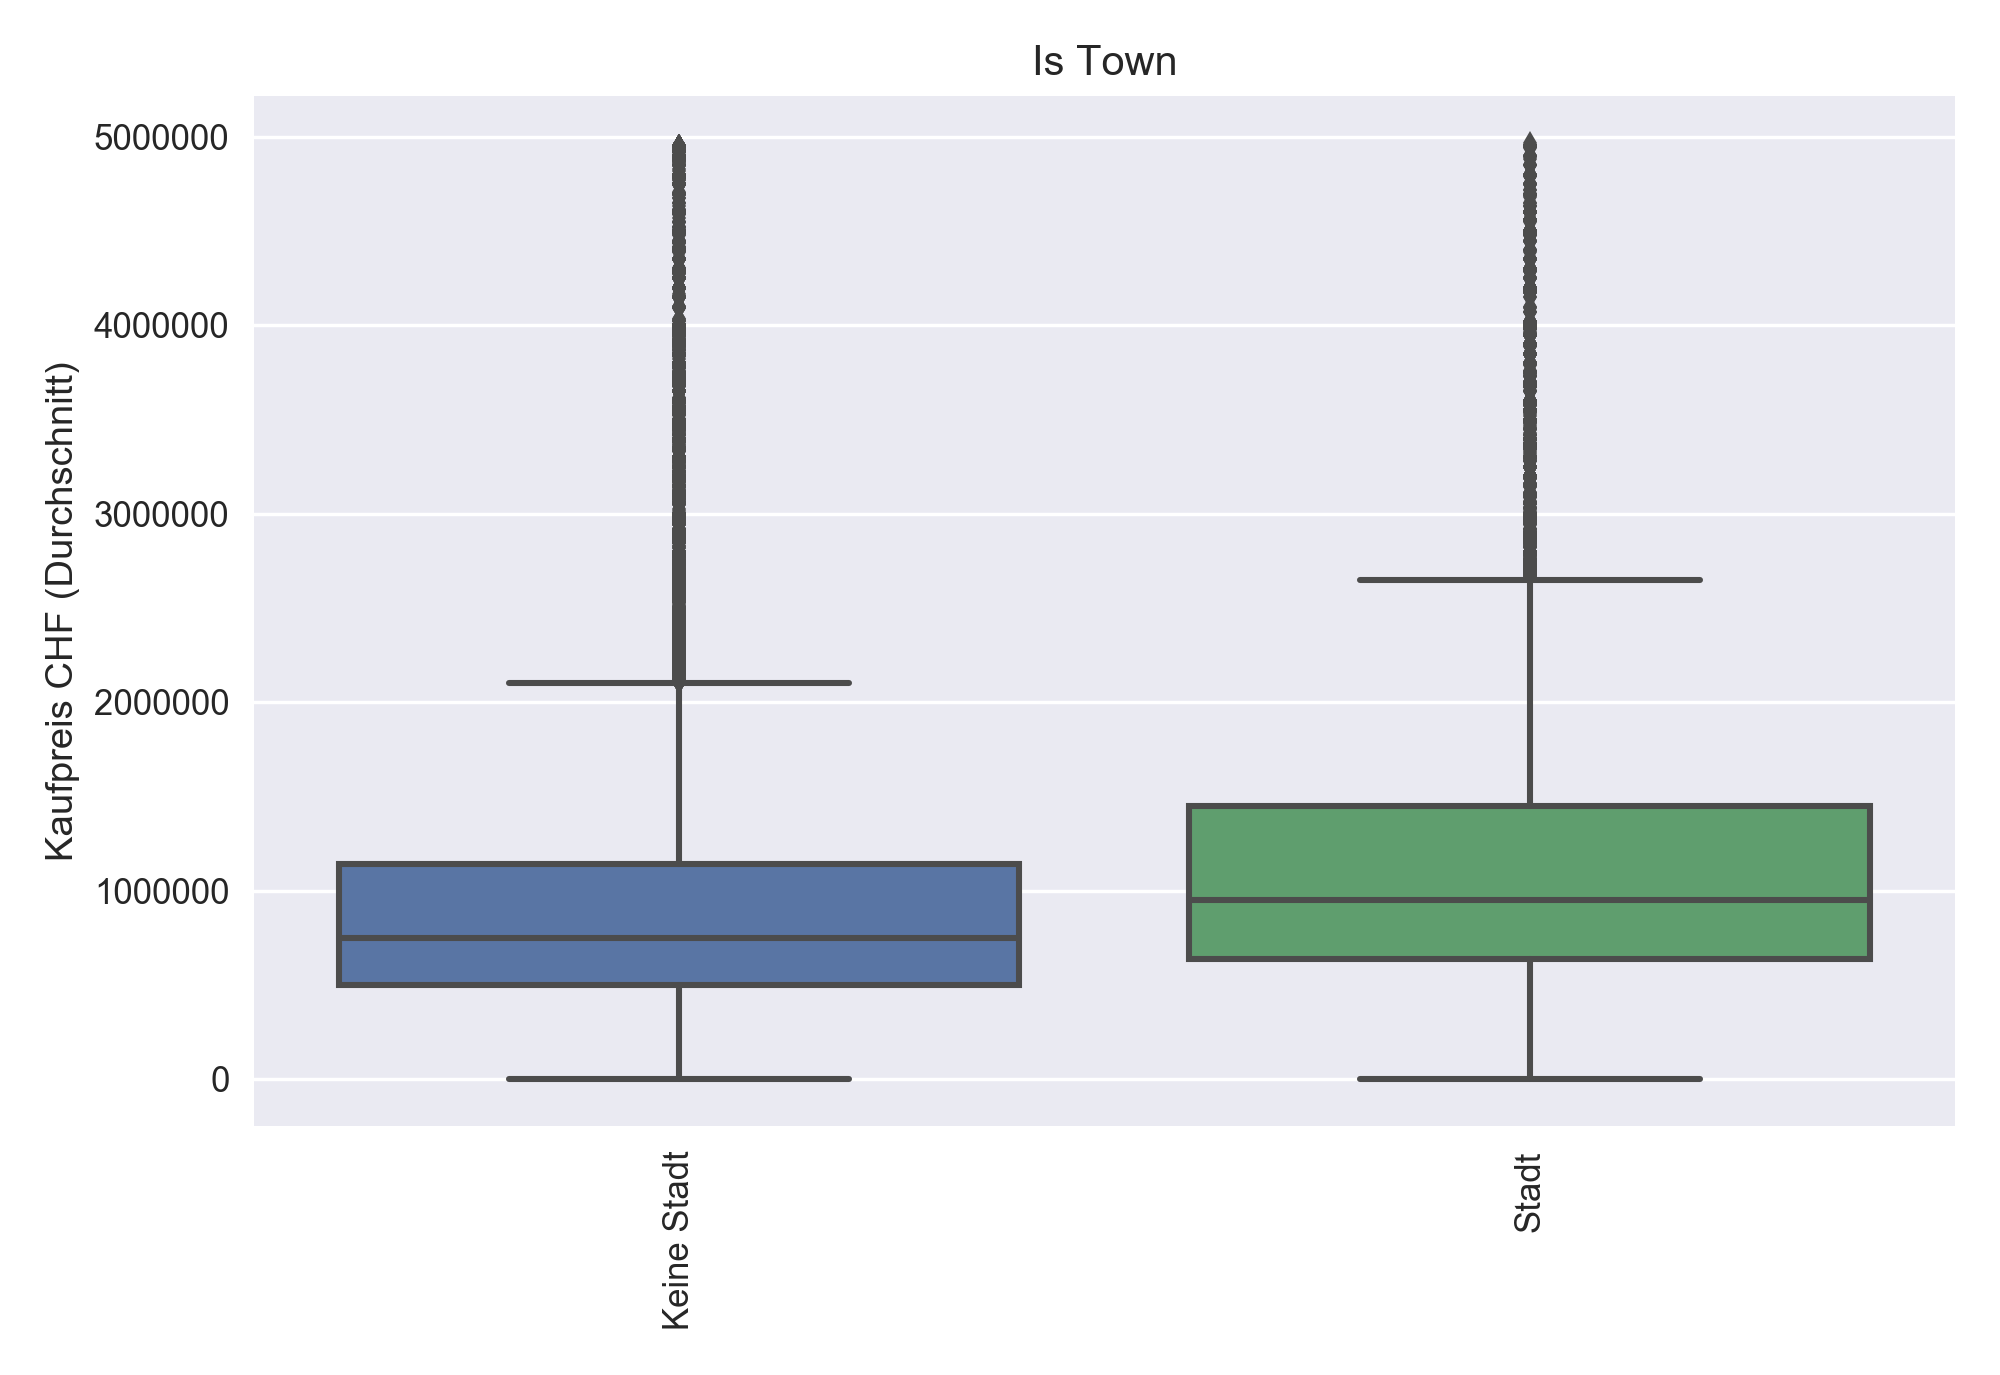
\includegraphics[width=\linewidth]{images/anhang/analysis/boxplot_is_town.png}
  \caption{Ist eine Stadt} 
\end{subfigure}
\begin{subfigure}{.5\textwidth}
  \centering
  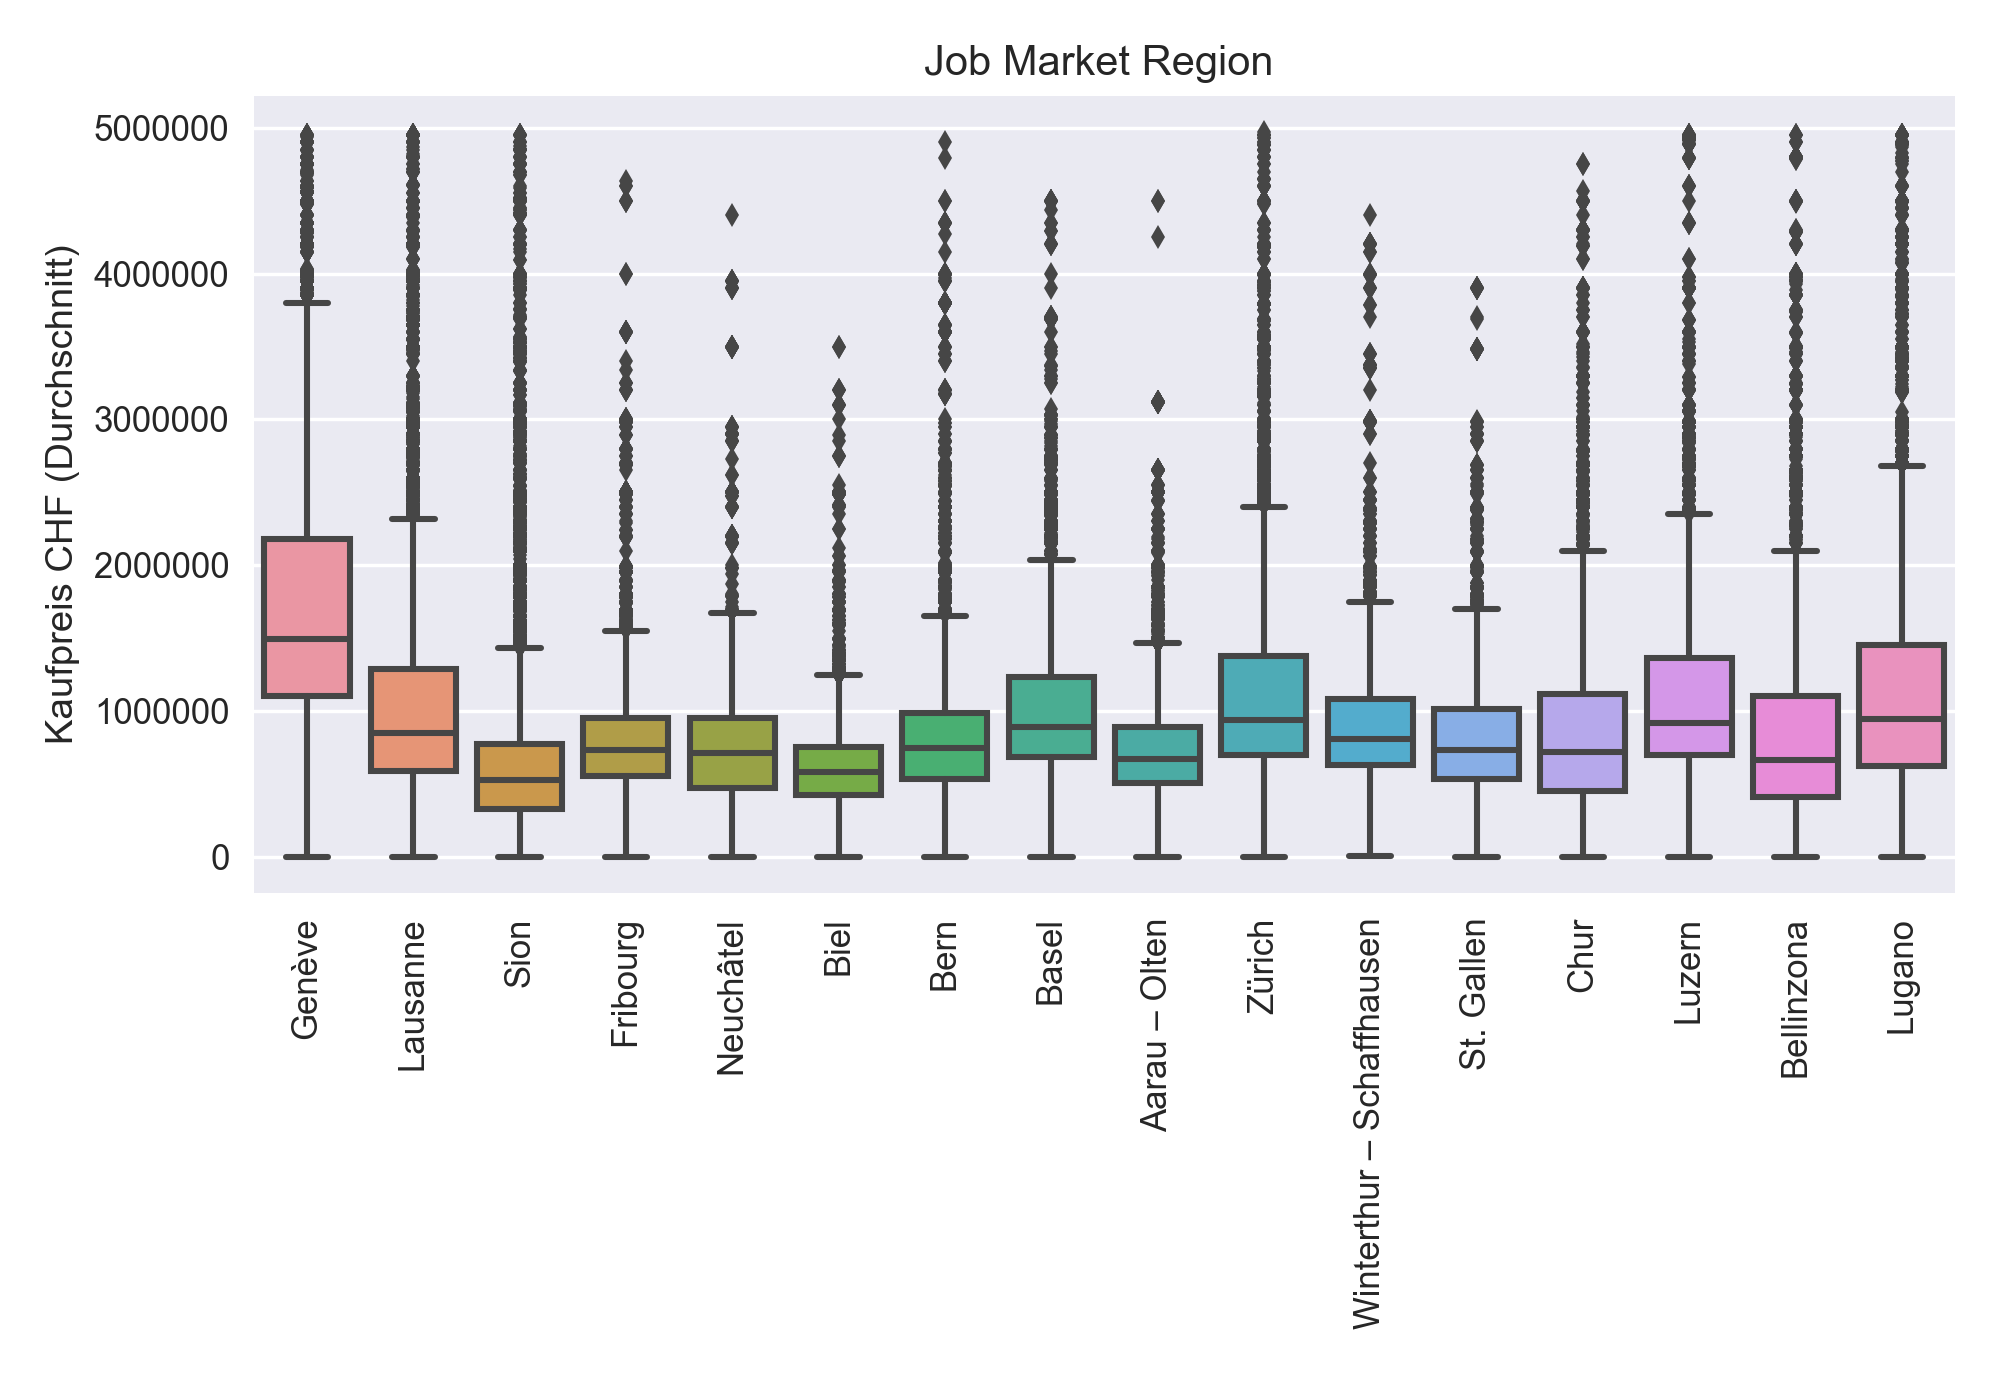
\includegraphics[width=\linewidth]{images/anhang/analysis/boxplot_job_market_region_id.png}
  \caption{Jobregionen}
\end{subfigure}
\begin{subfigure}{.5\textwidth}
  \centering
  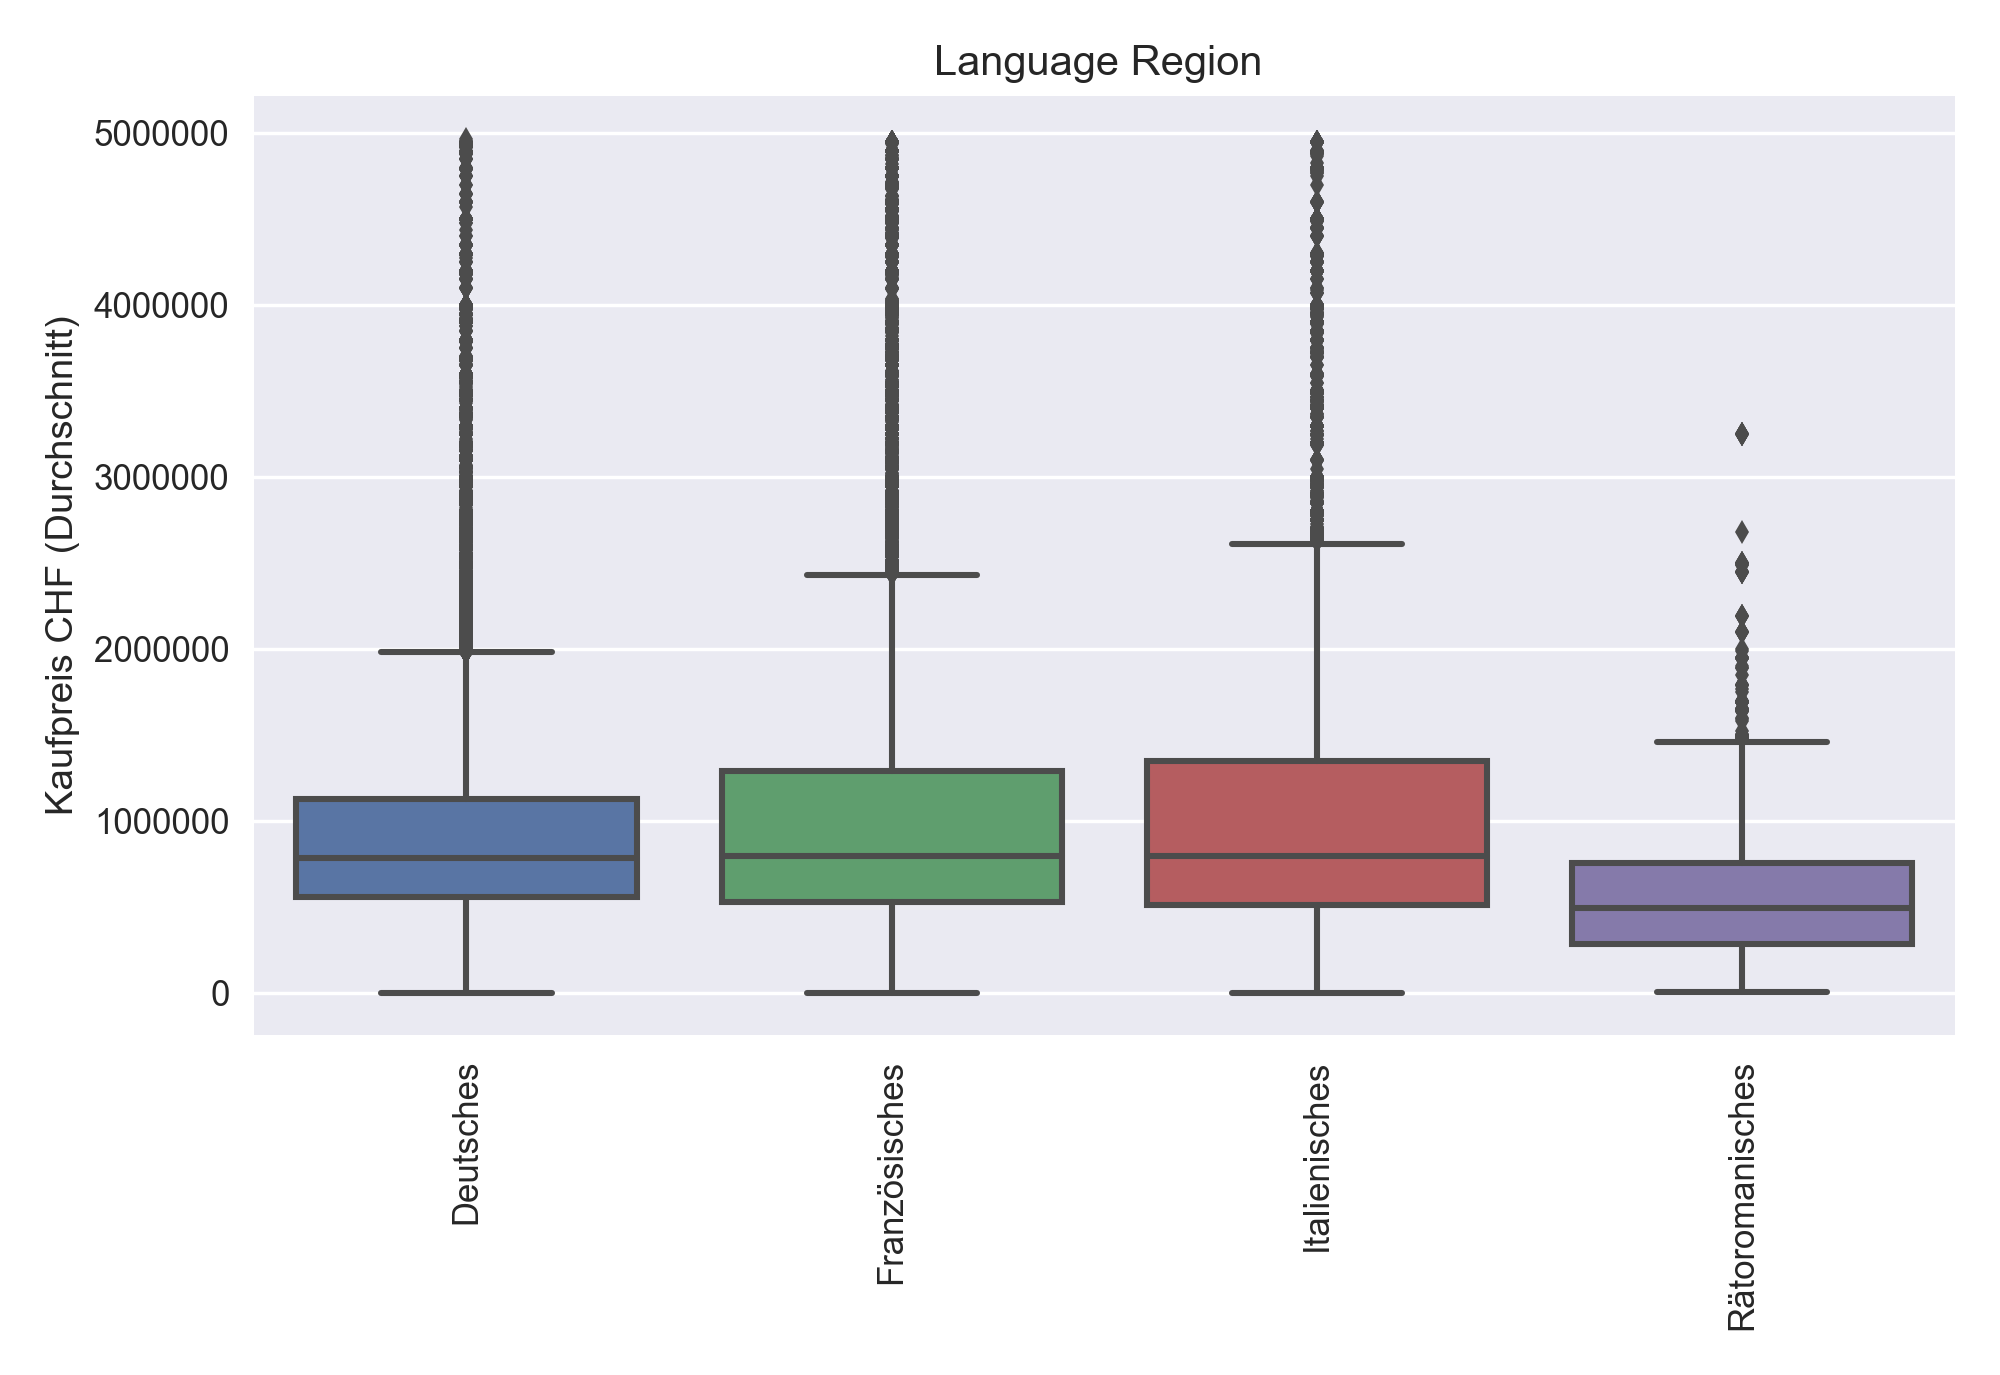
\includegraphics[width=\linewidth]{images/anhang/analysis/boxplot_language_region_id.png}
  \caption{Sprachregionen} 
\end{subfigure}
\begin{subfigure}{.5\textwidth}
  \centering
  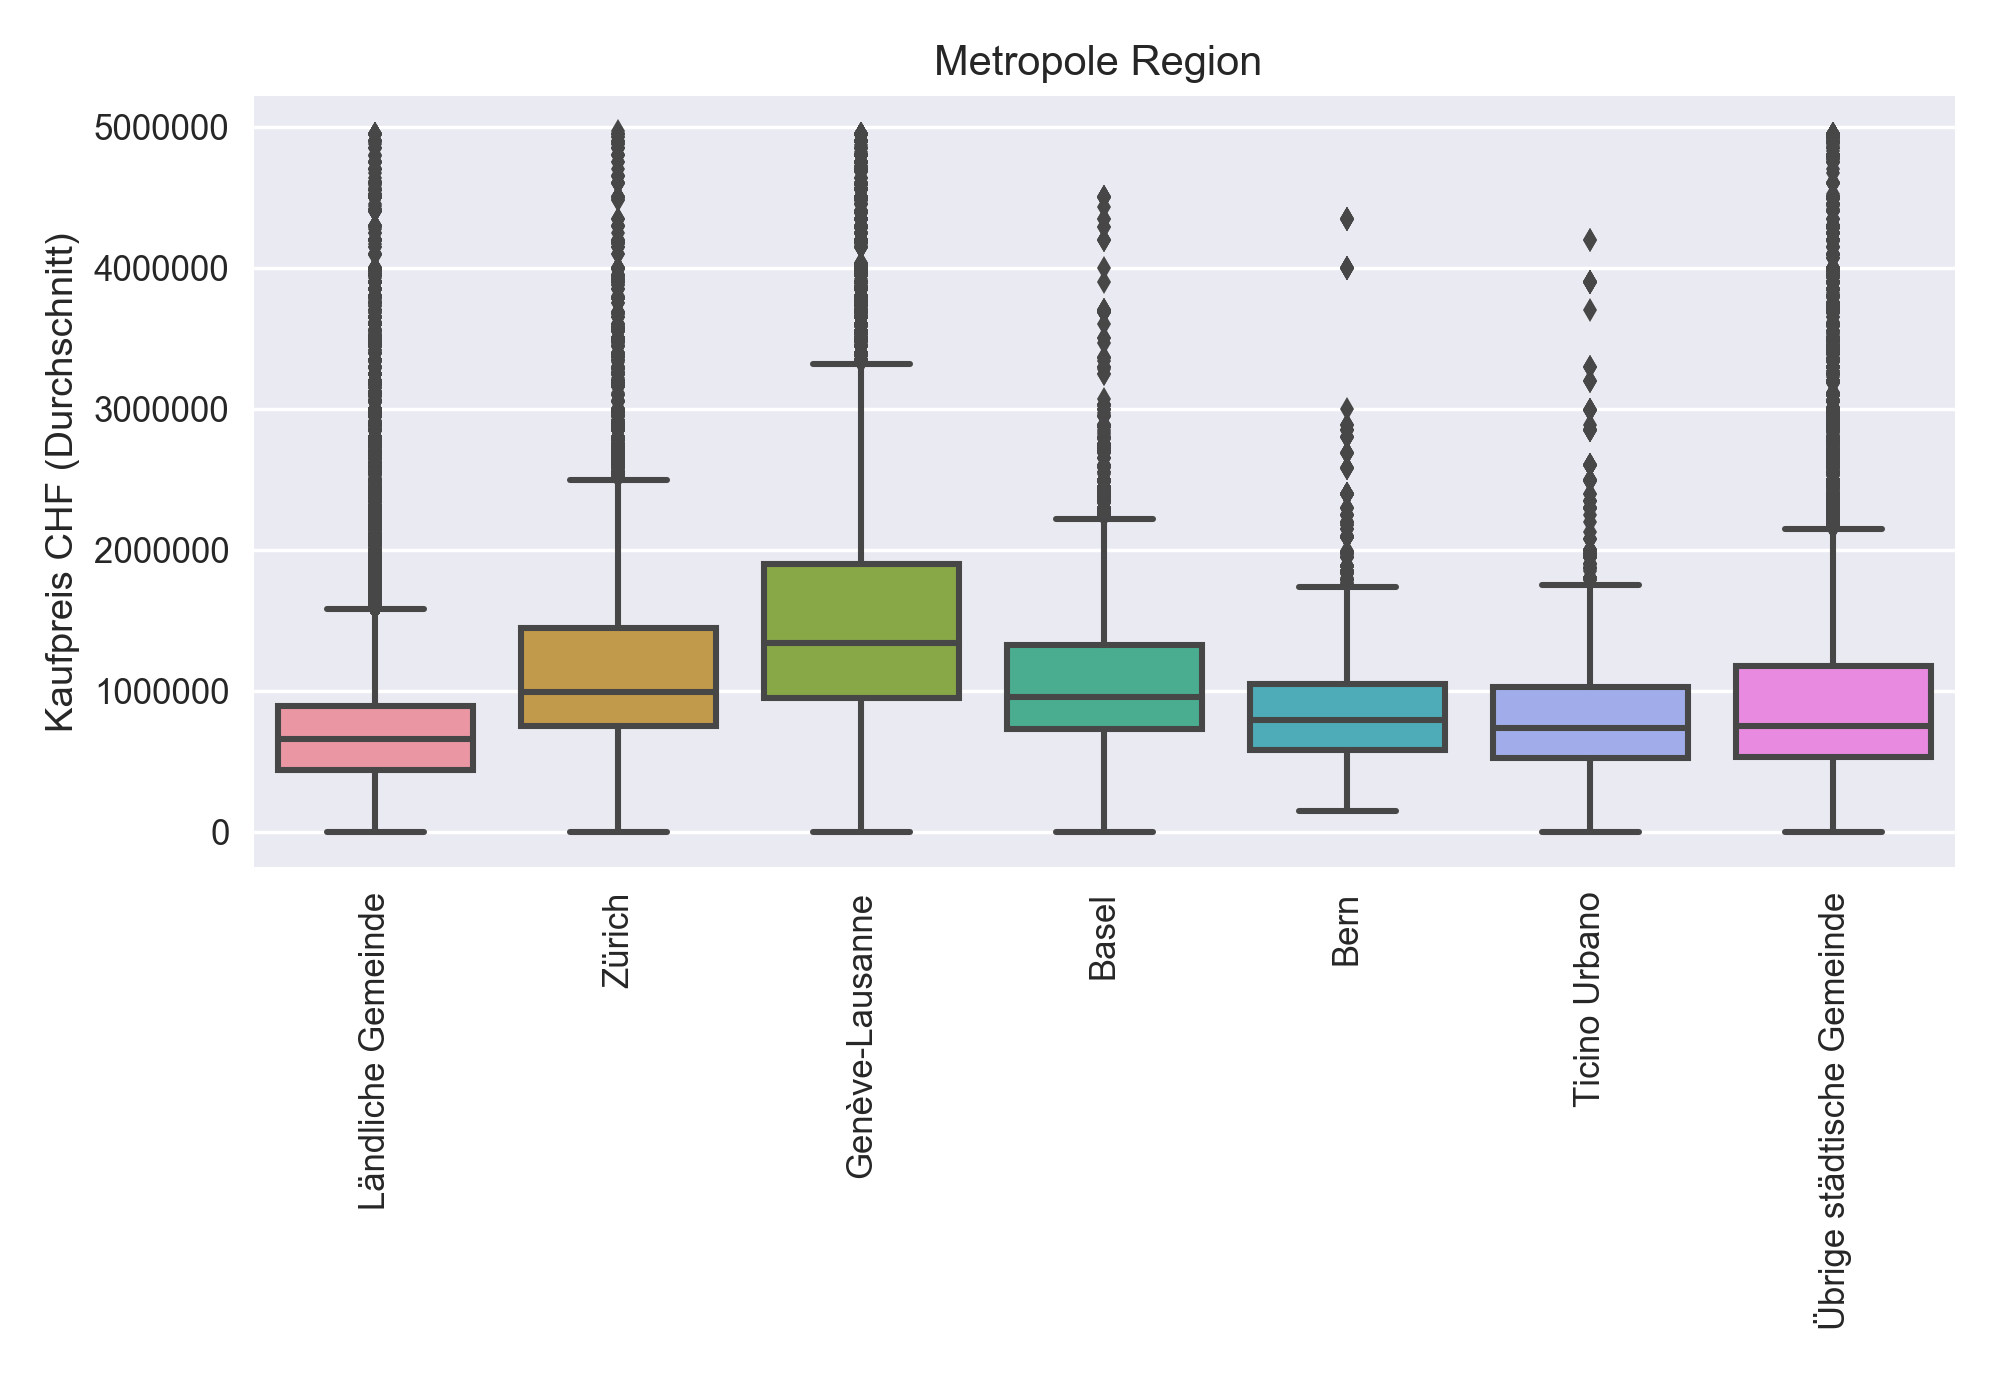
\includegraphics[width=\linewidth]{images/anhang/analysis/boxplot_metropole_region_id.png}
  \caption{Metropolregionen}
\end{subfigure}
\begin{subfigure}{.5\textwidth}
  \centering
  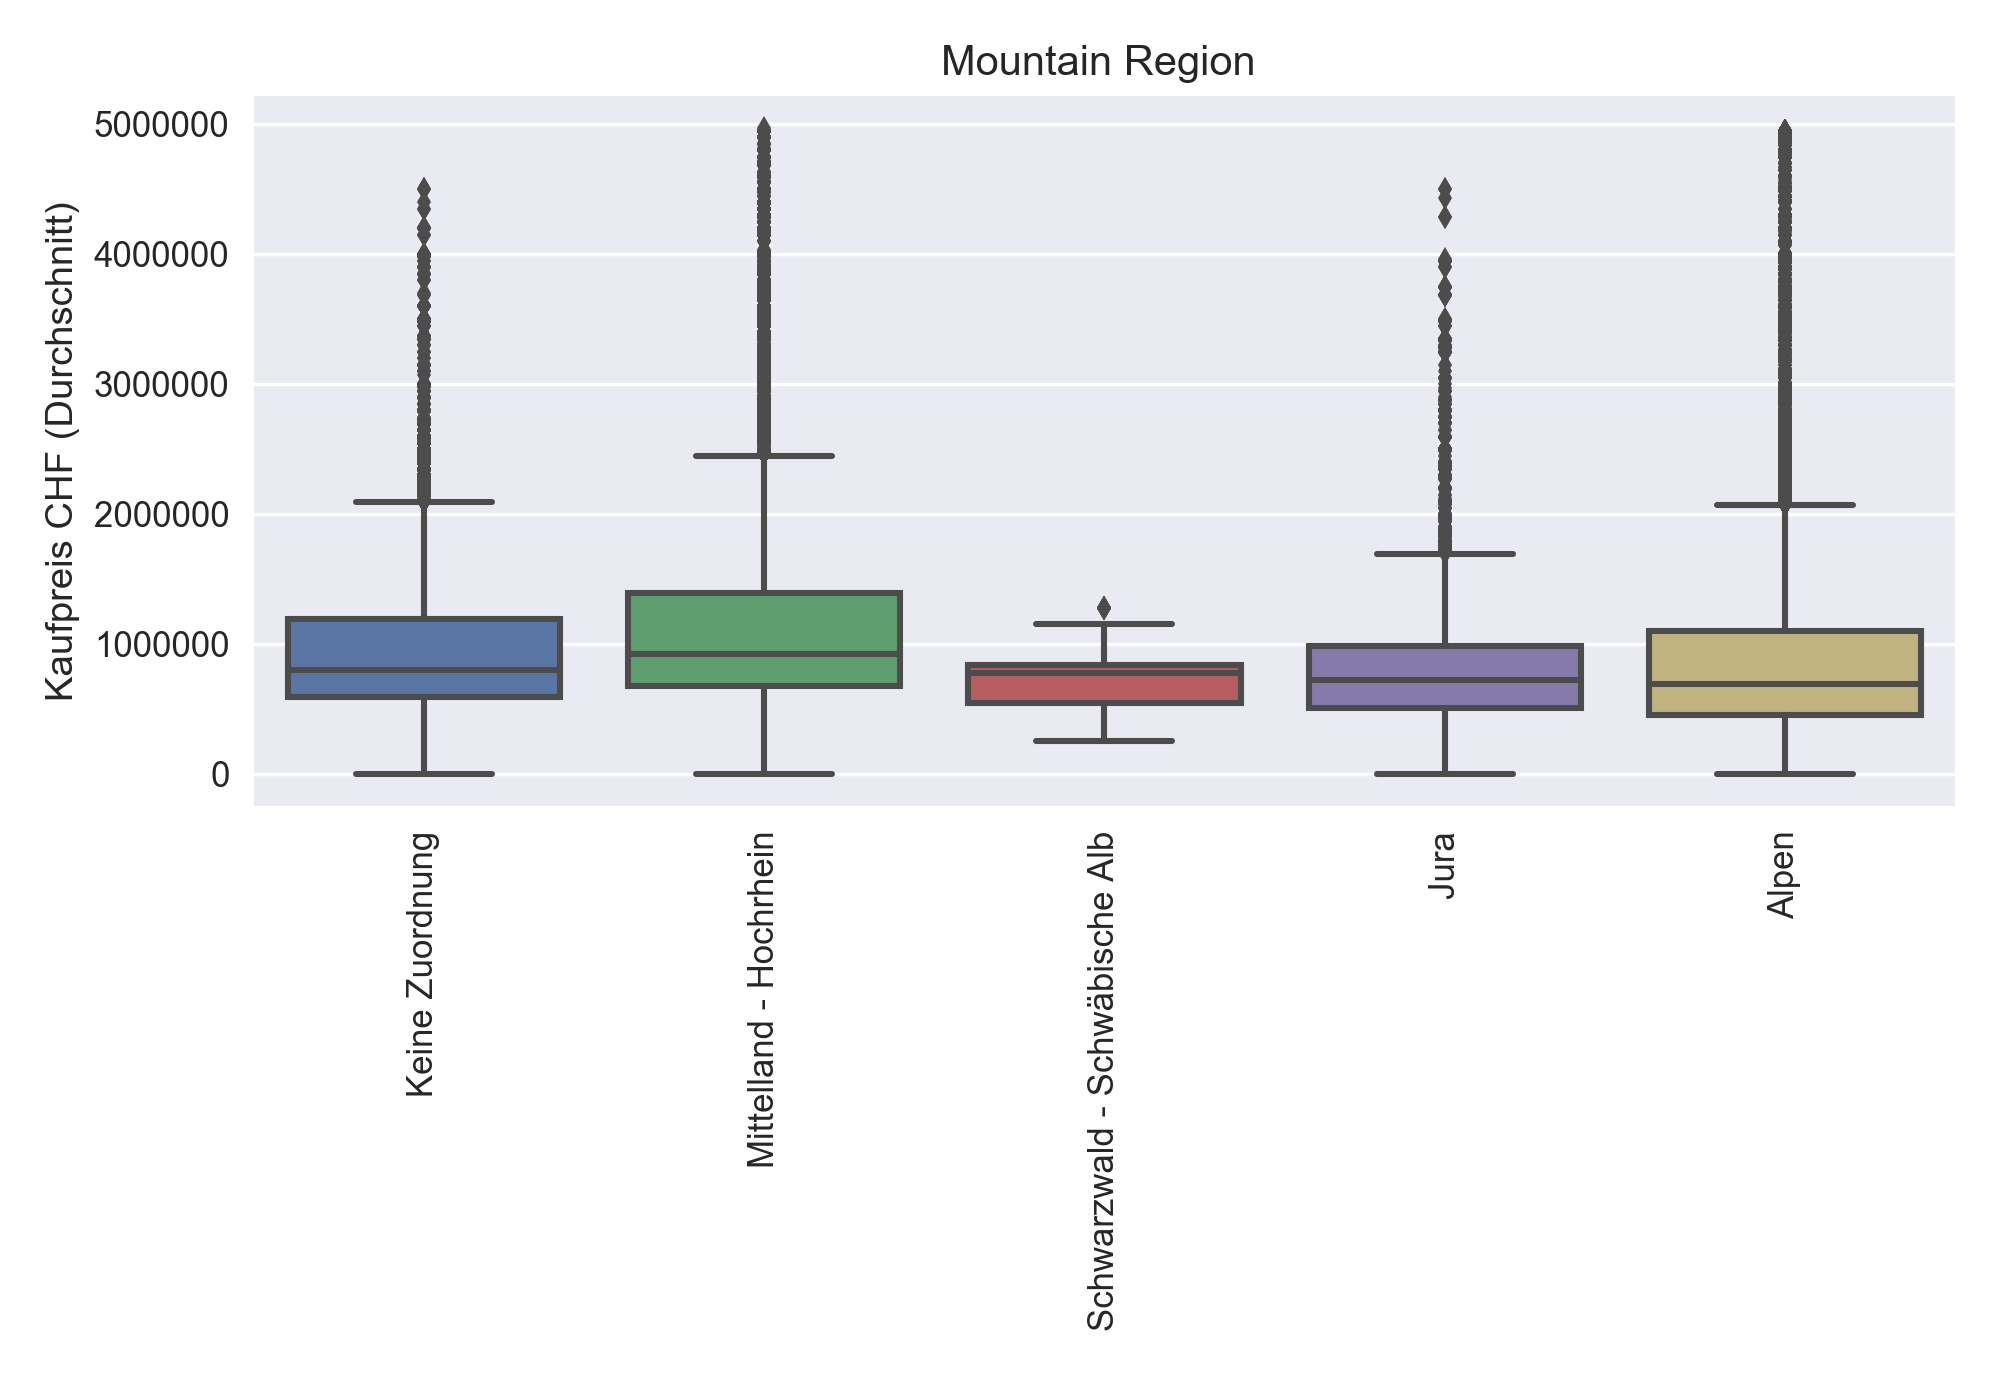
\includegraphics[width=\linewidth]{images/anhang/analysis/boxplot_mountain_region_id.png}
  \caption{Bergregionen} 
\end{subfigure}
\caption{Boxplots für ortsbezogene Kategorien 1}
\end{figure}

\begin{figure}[h]
\begin{subfigure}{.5\textwidth}
  \centering
  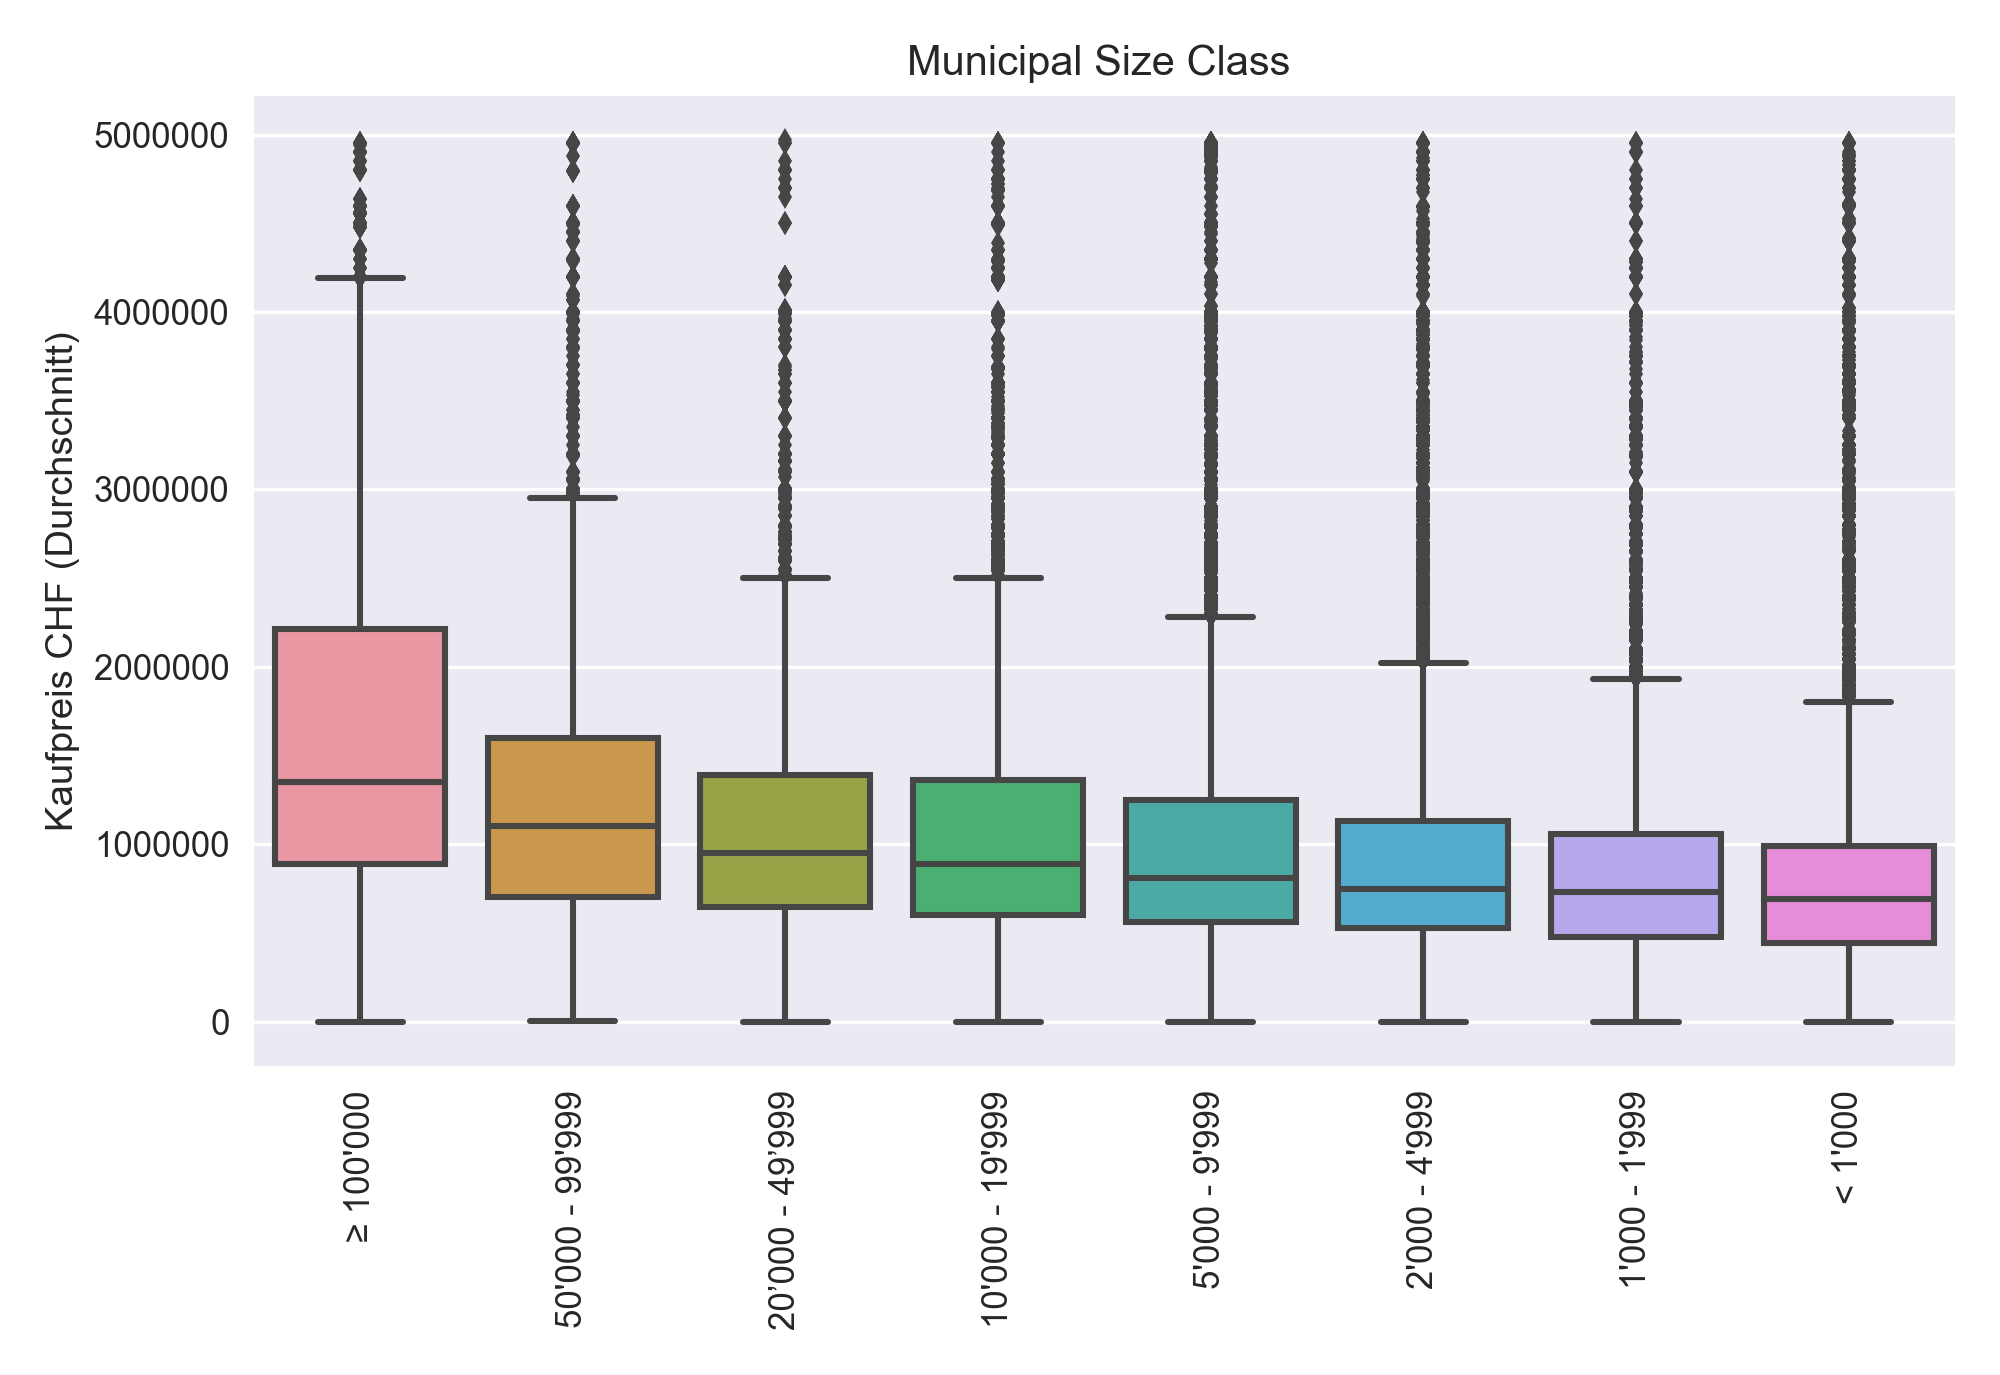
\includegraphics[width=\linewidth]{images/anhang/analysis/boxplot_municipal_size_class_id.png}
  \caption{Gemeindegrössen}
\end{subfigure}
\begin{subfigure}{.5\textwidth}
  \centering
  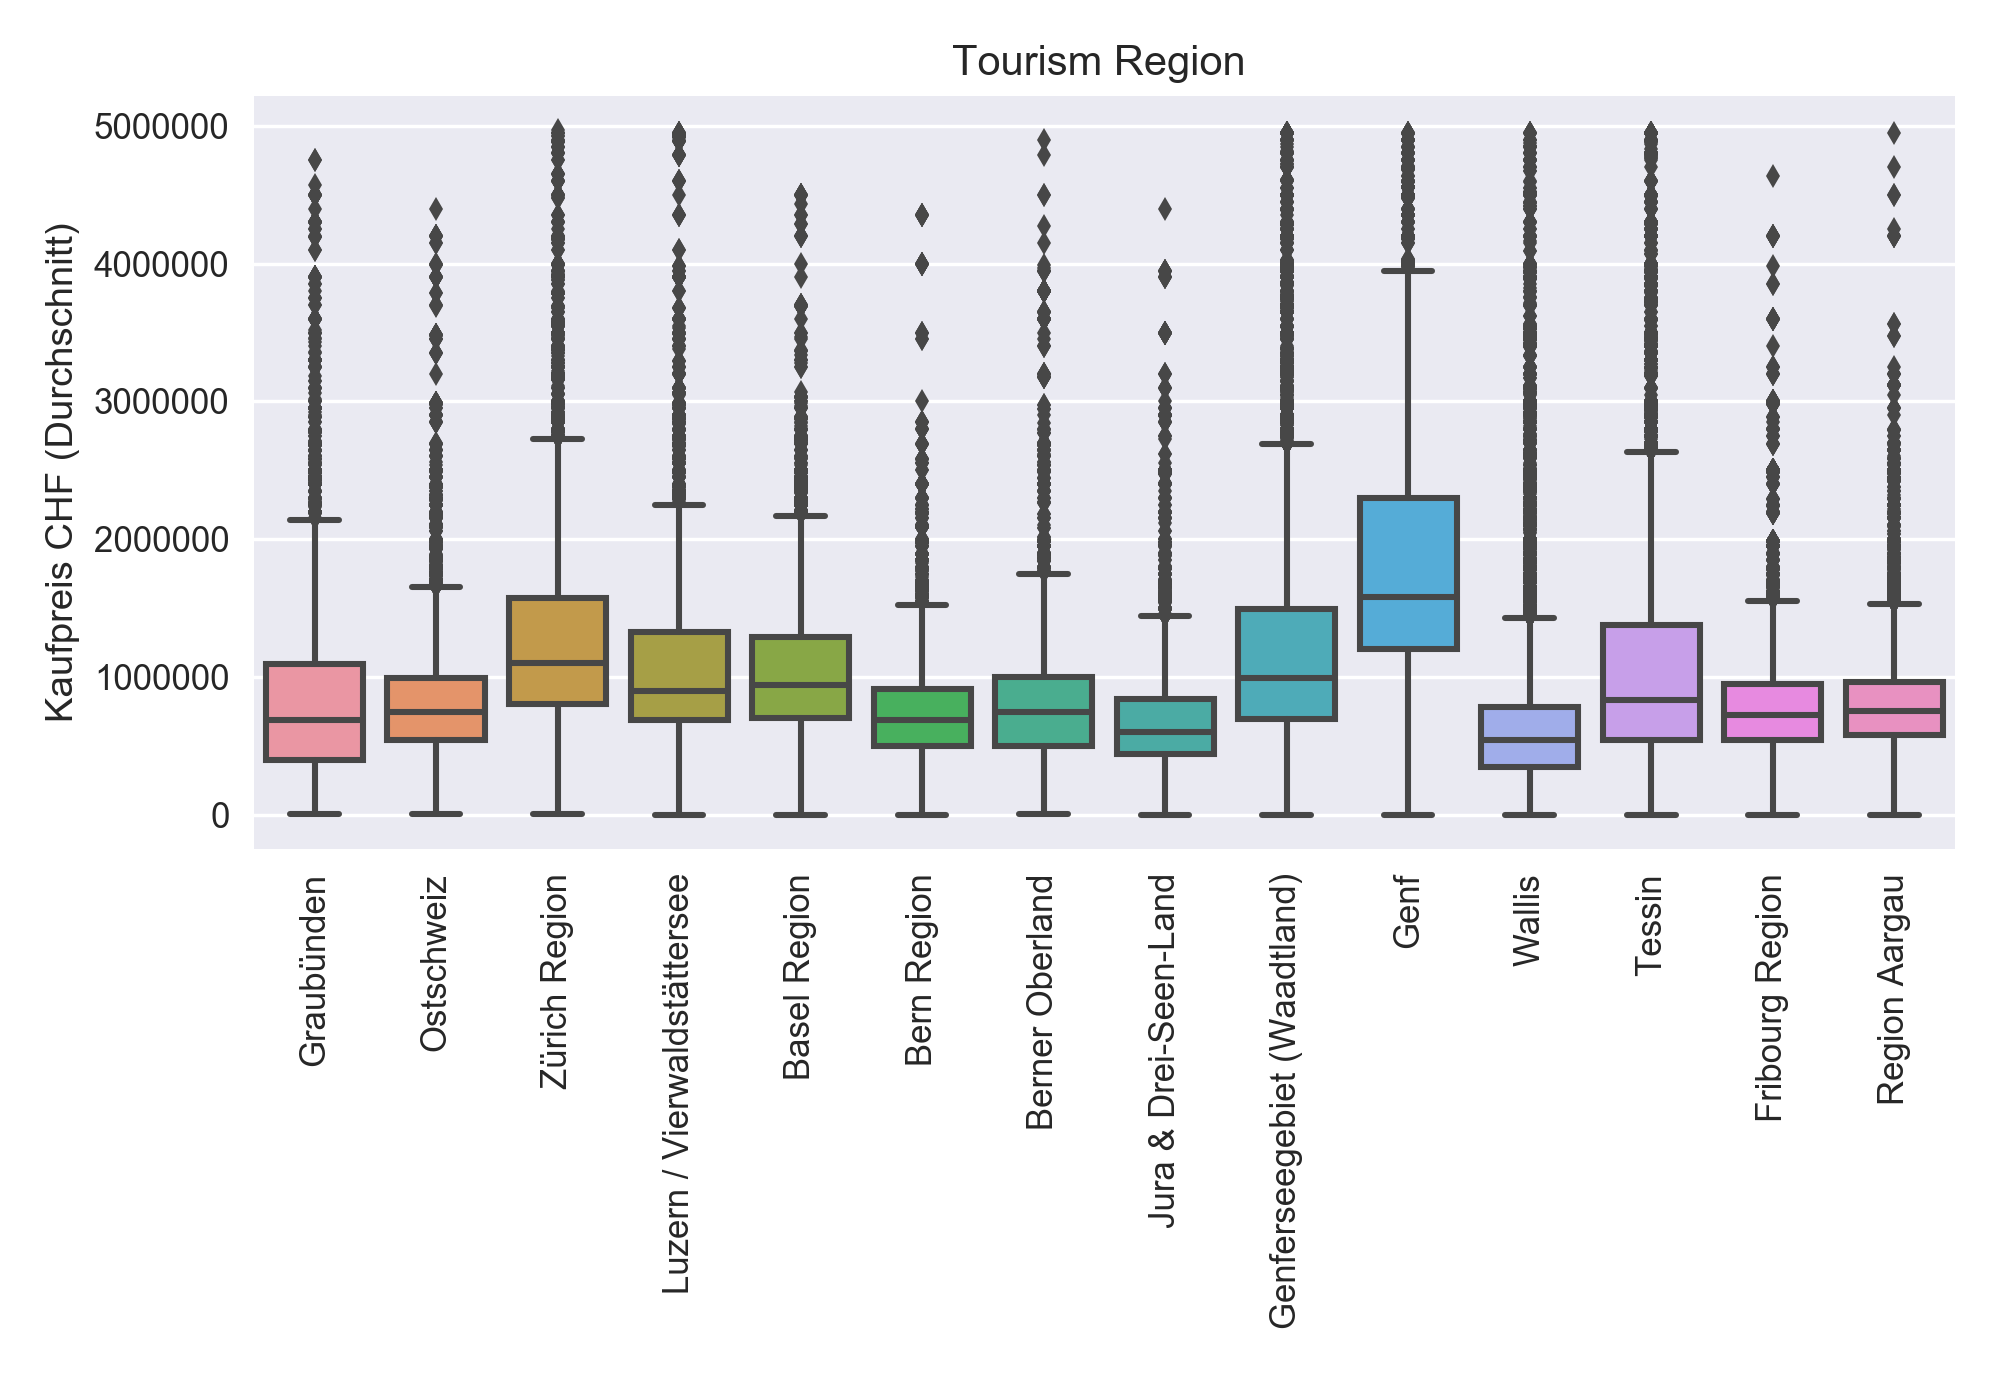
\includegraphics[width=\linewidth]{images/anhang/analysis/boxplot_tourism_region_id.png}
  \caption{Tourismusregionen} 
\end{subfigure}
\caption{Boxplots für ortsbezogene Kategorien 2}
\end{figure}

\begin{figure}[h]
  \centering
  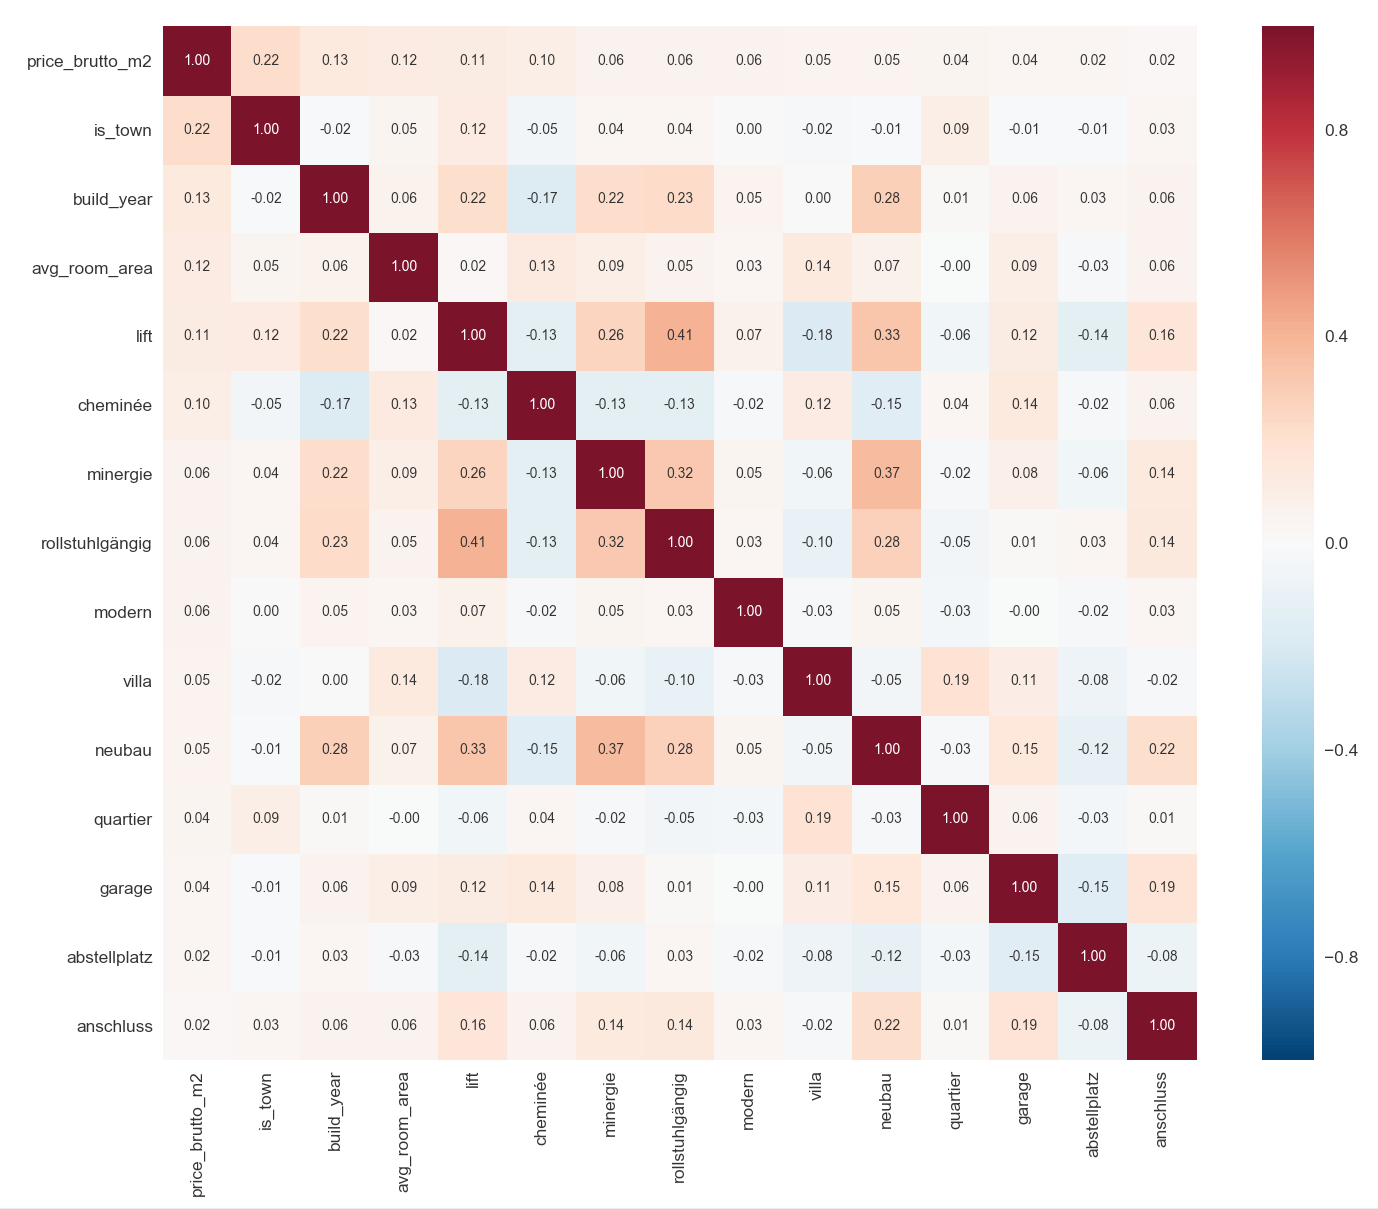
\includegraphics[width=\linewidth]{images/anhang/analysis/HeatMap_Importance.png}
  \caption{Heatmap mit Zahlen der Korrelation}
  \end{figure}
  
\begin{figure}[h]
  \centering
  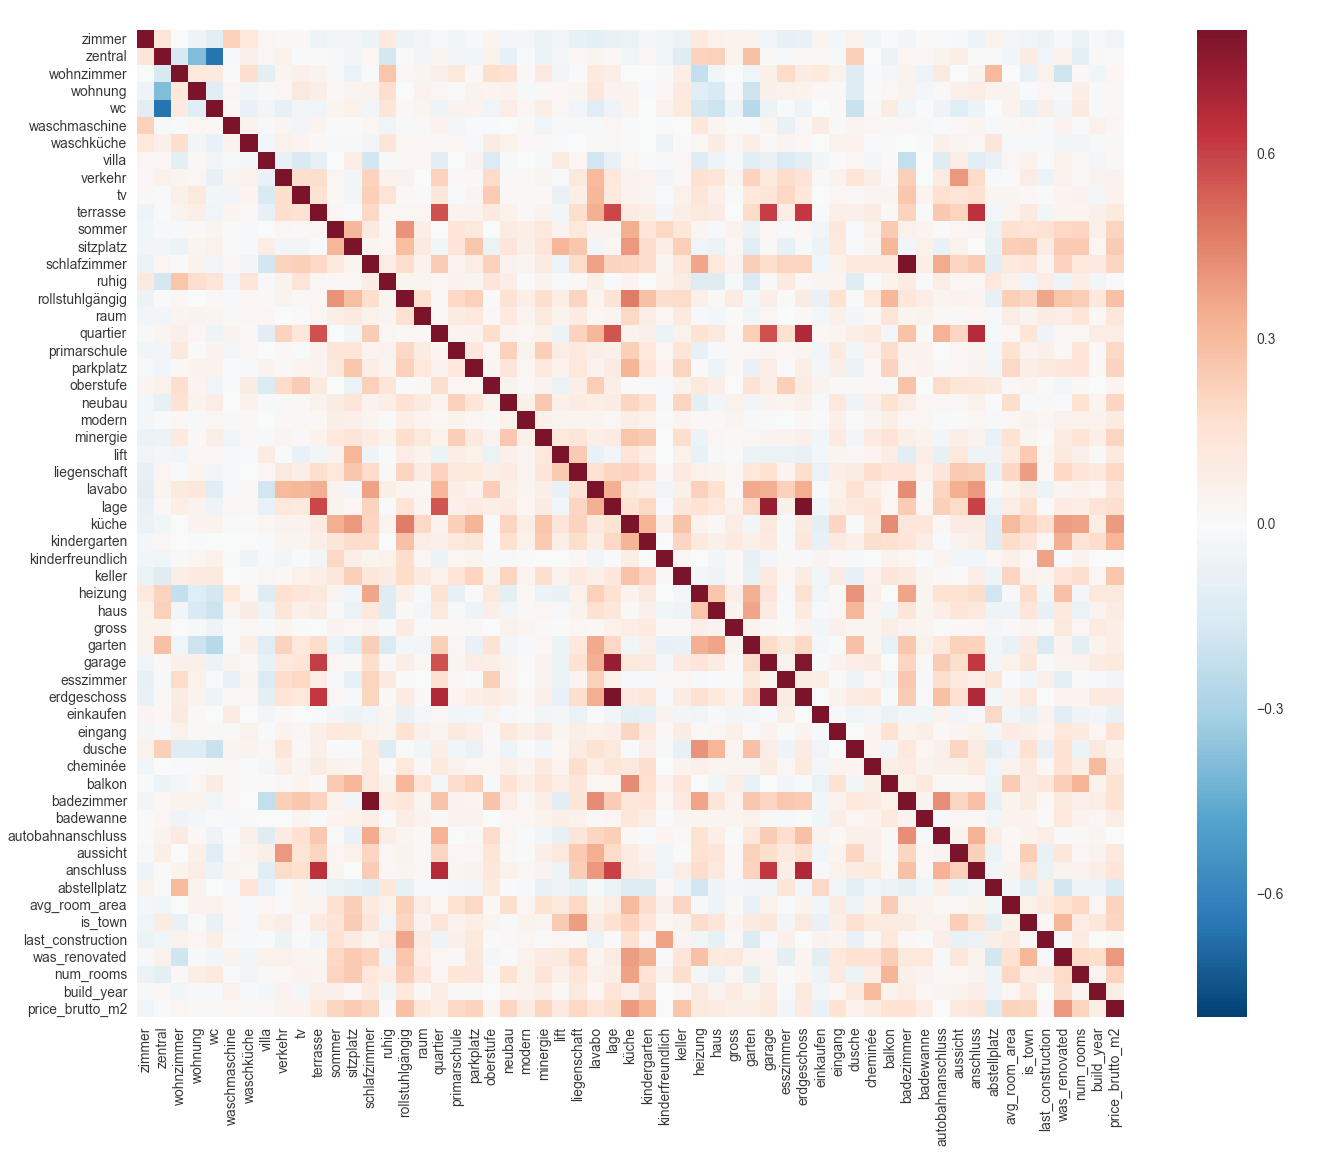
\includegraphics[width=\linewidth]{images/anhang/analysis/HeatMap_all.png}
  \caption{Heatmap mit Tags} 
\end{figure}

\begin{figure}[h]
  \centering
  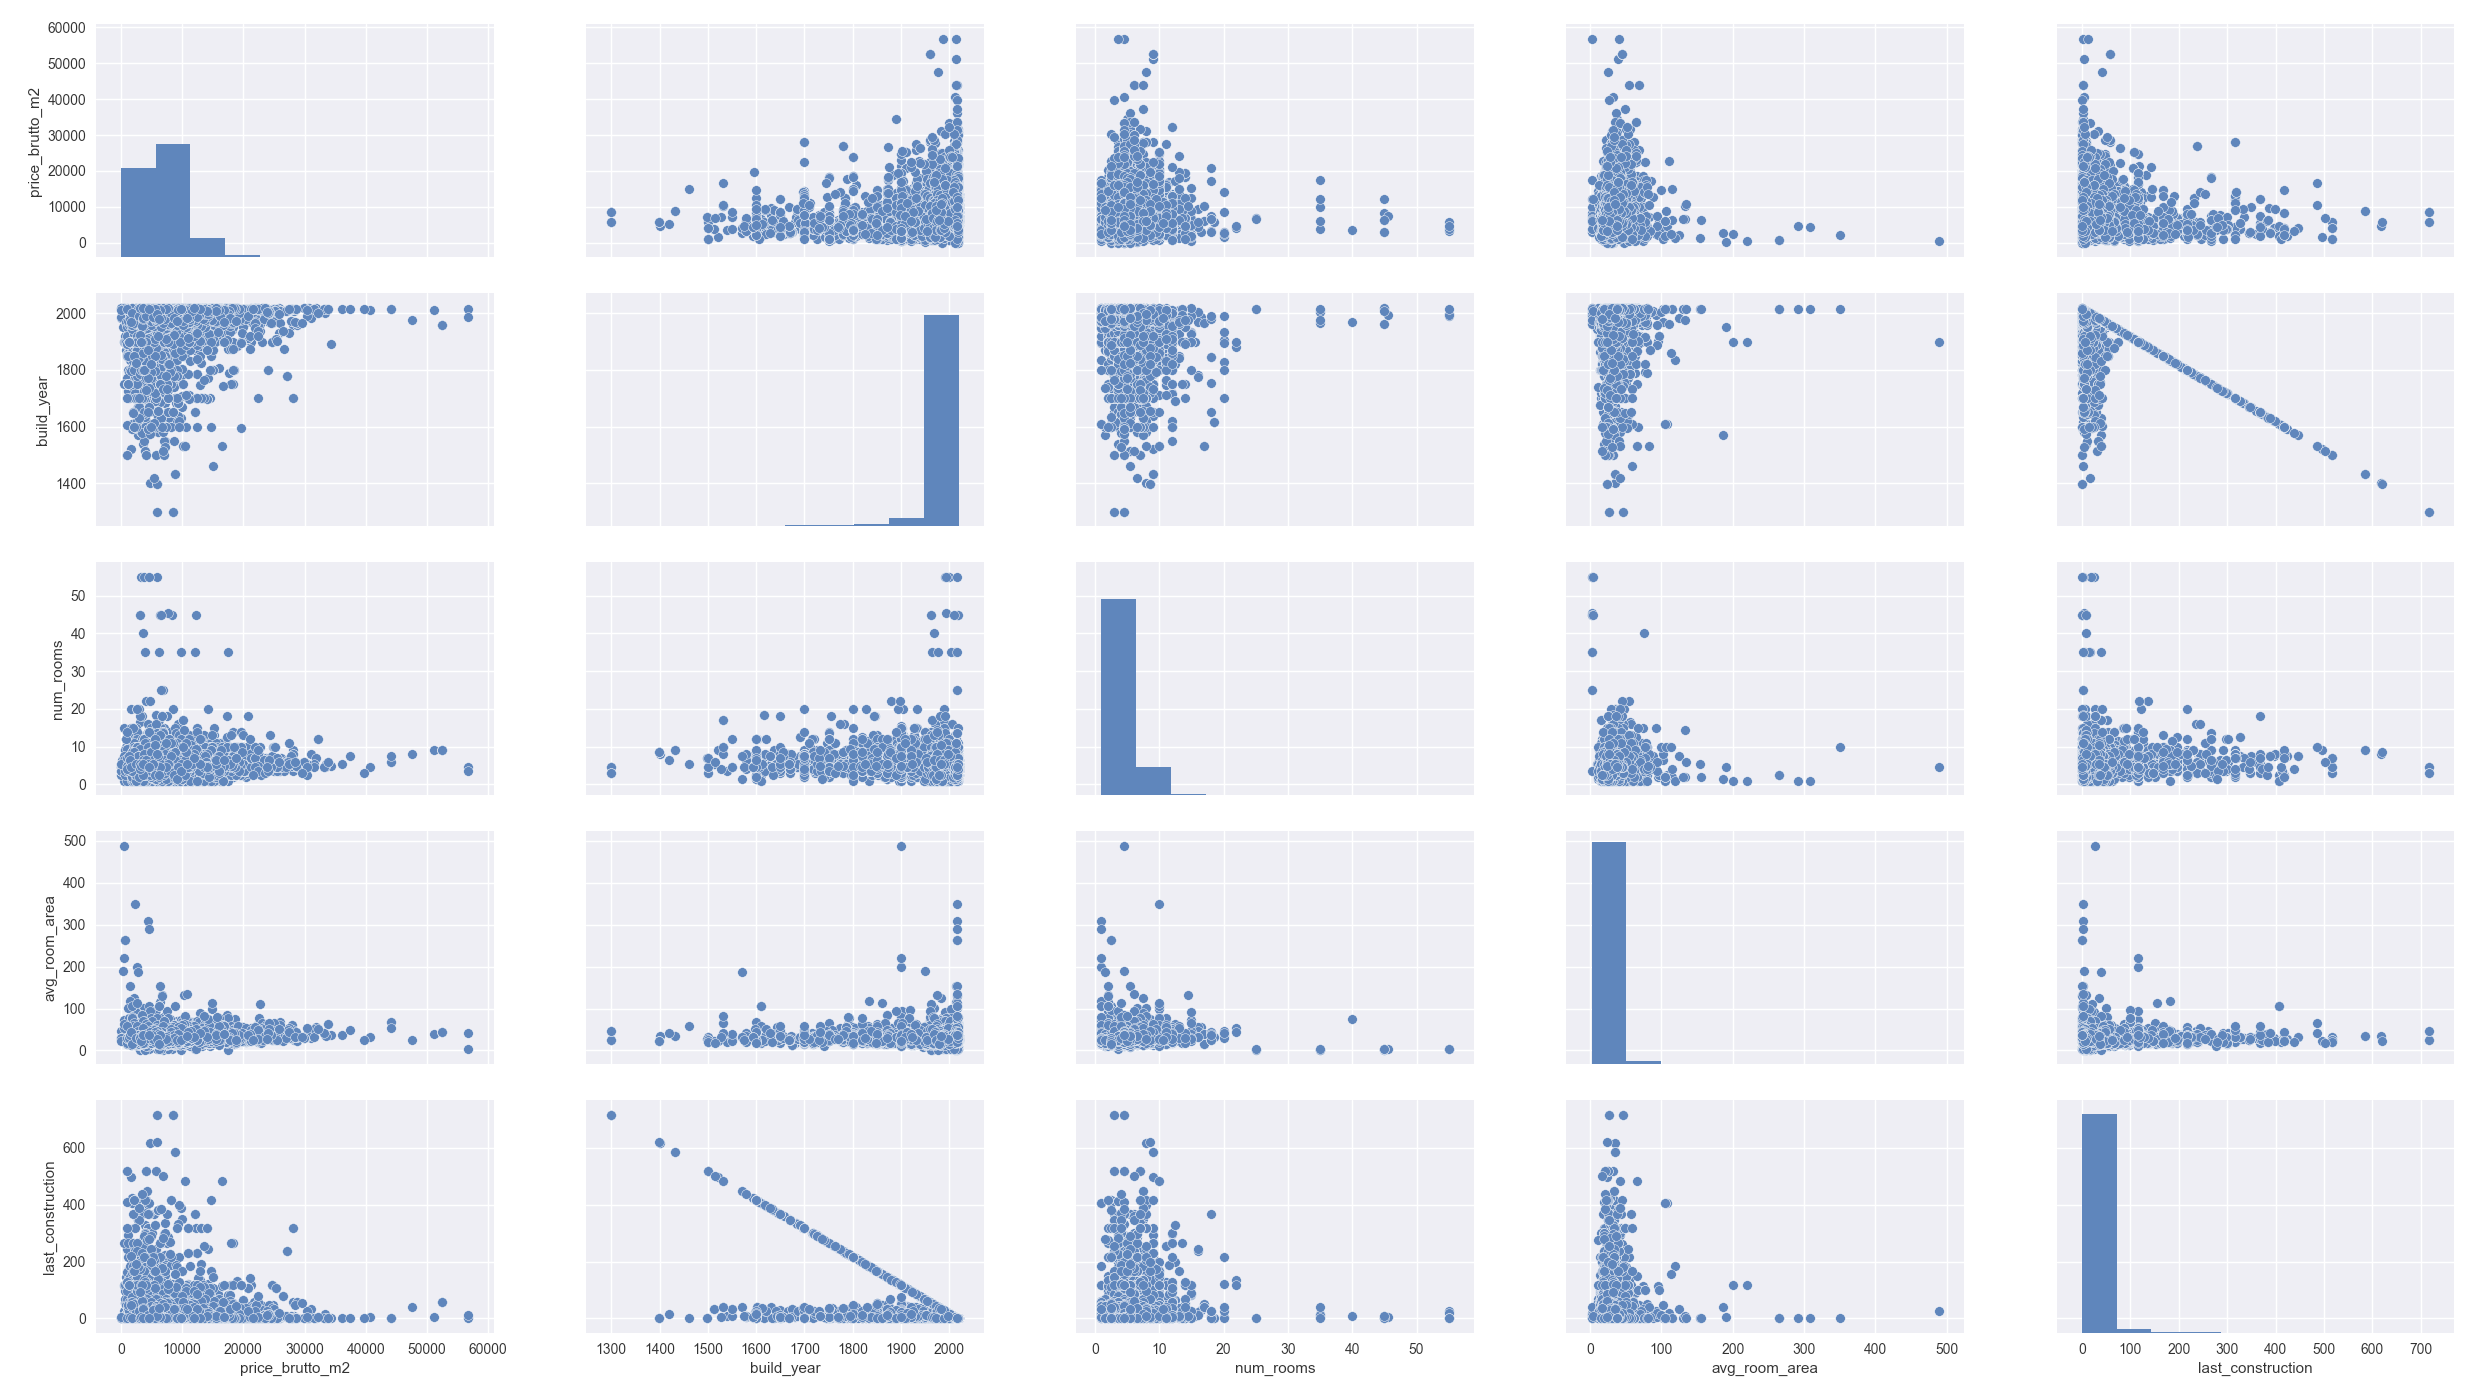
\includegraphics[width=\linewidth]{images/anhang/analysis/cross.png}
  \caption{Vergleich aller nummerischen Features} 
\end{figure}


\begin{figure}[h]
  \centering
  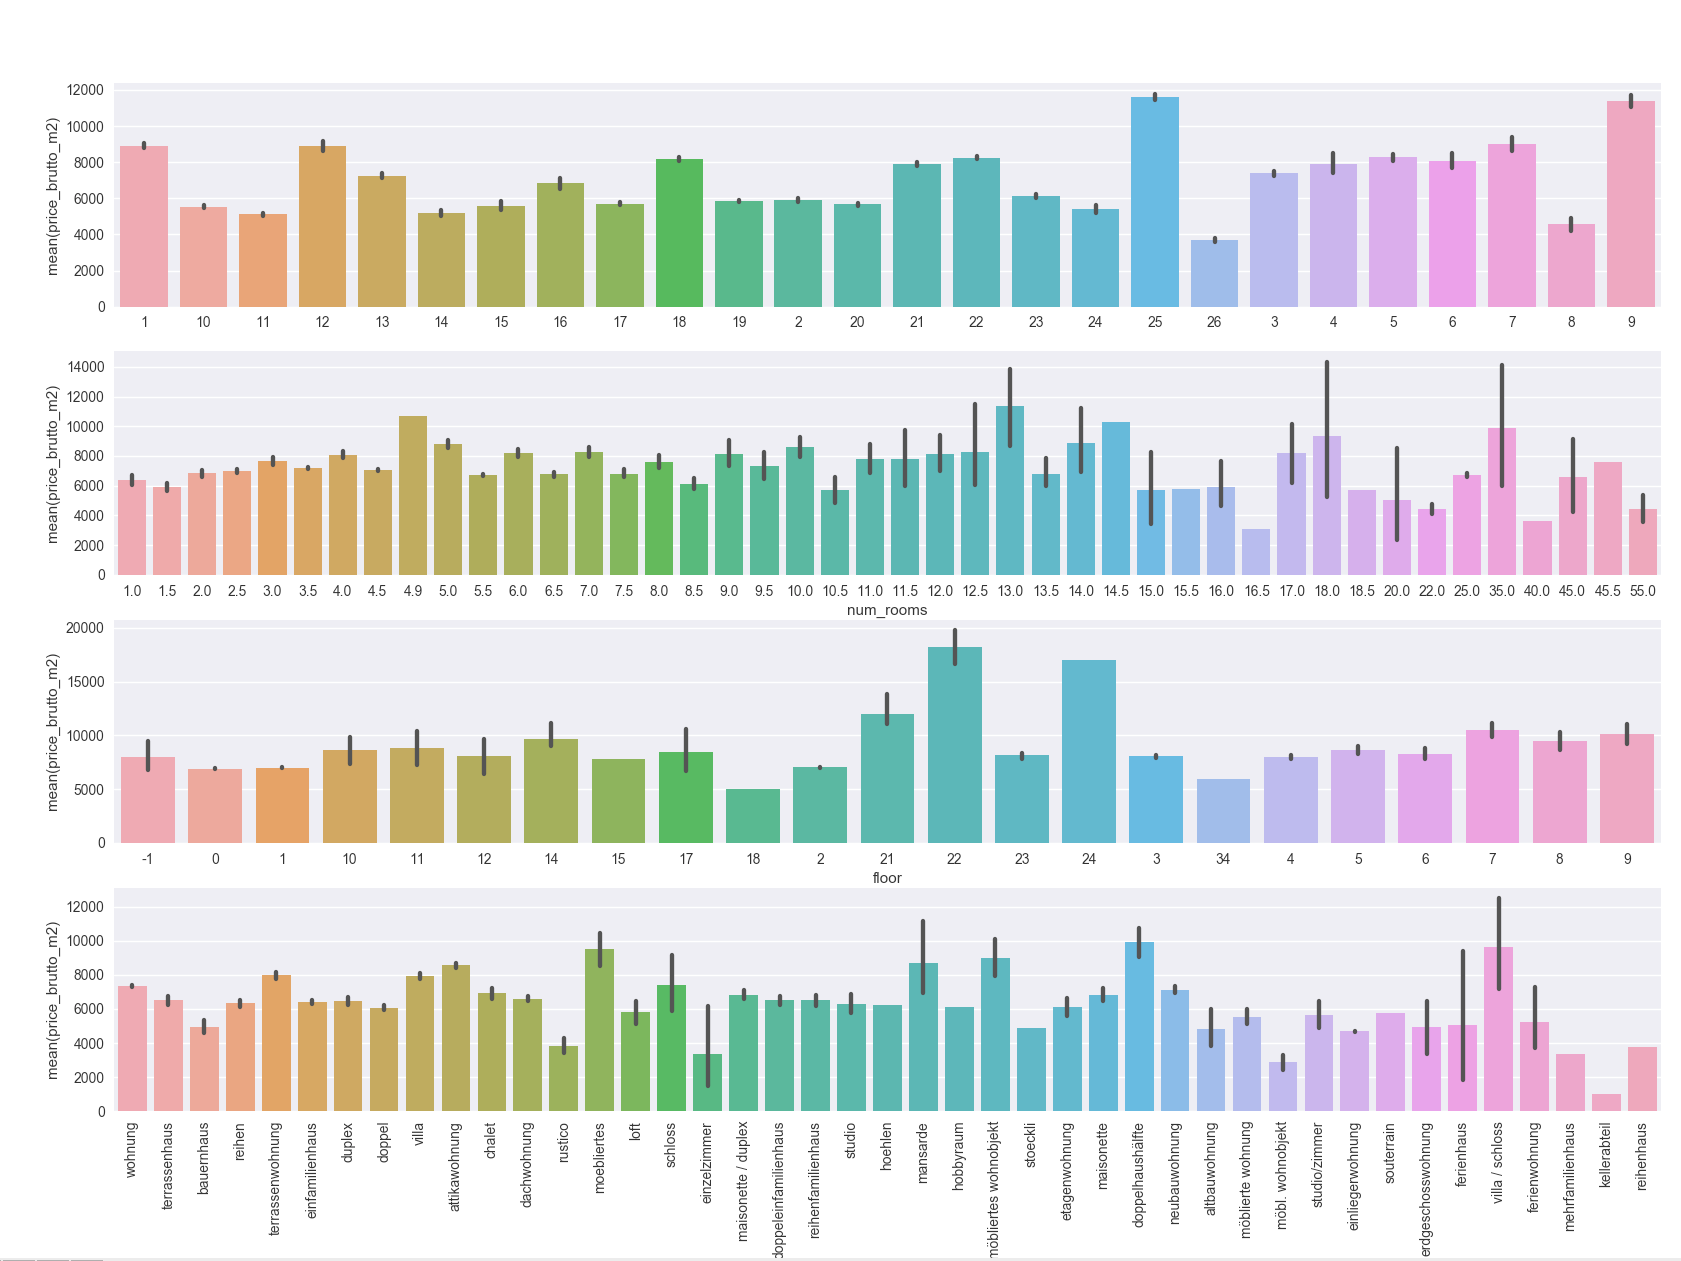
\includegraphics[width=\linewidth]{images/anhang/analysis/Verteilung.png}
  \caption{Verteilung der nummerischen Features} 
\end{figure}



\begin{figure}[h]
  \begin{subfigure}{.5\textwidth}
    \centering
    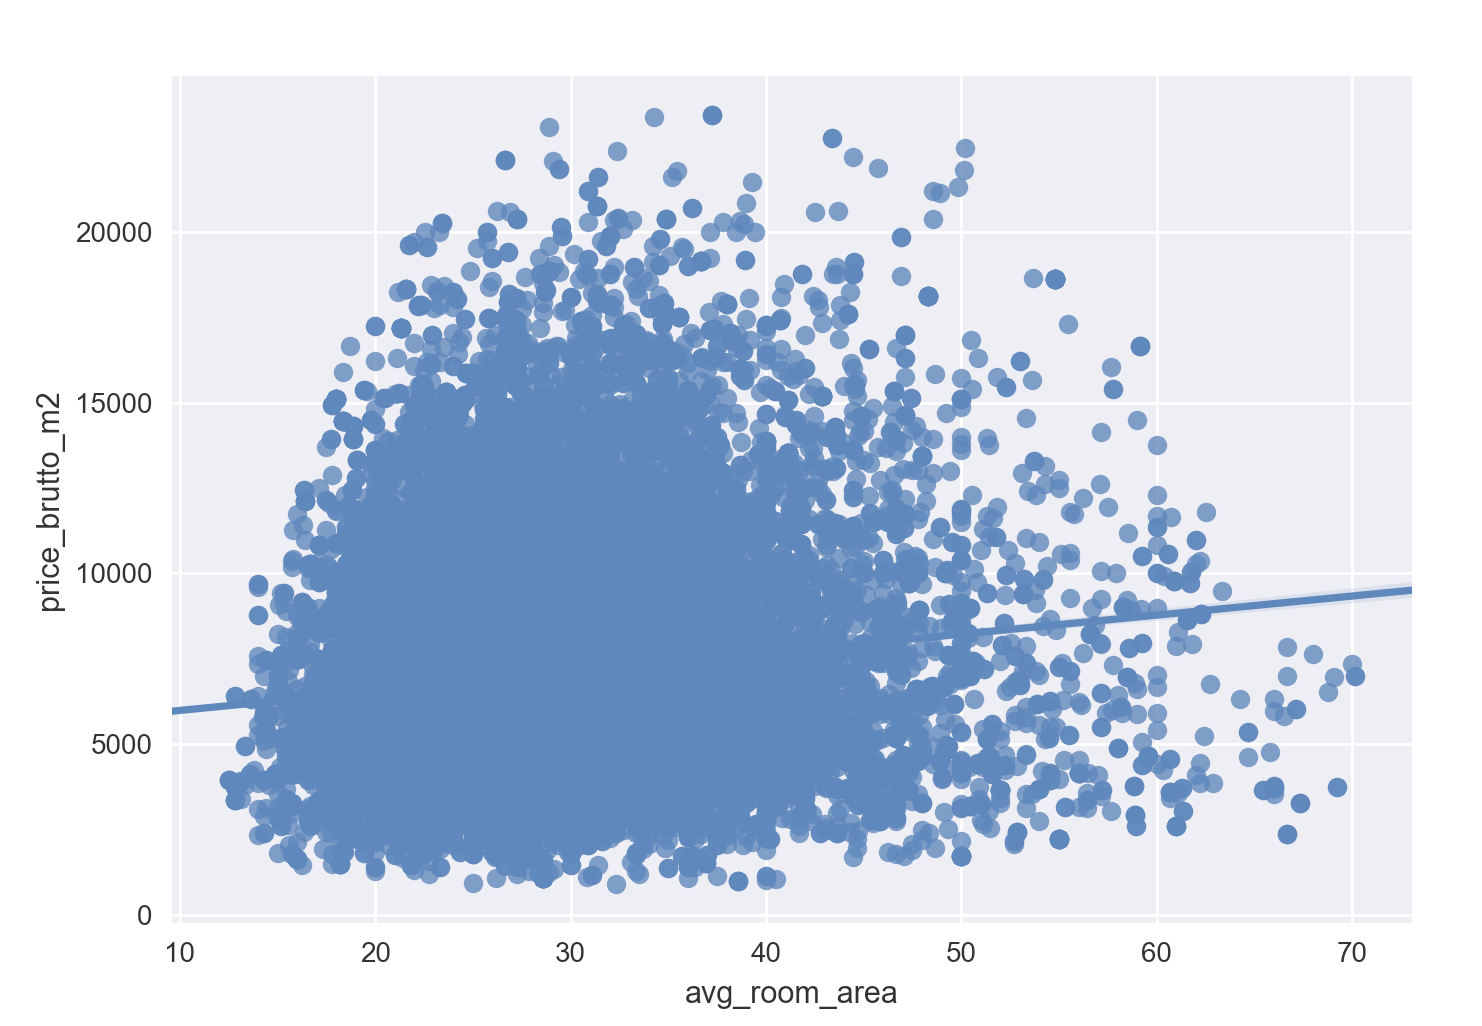
\includegraphics[width=\linewidth]{images/anhang/analysis/avg_room_to_price.png}
    \caption{Durchschnittliche Raumgrösse zu Preis}
  \end{subfigure}
  \begin{subfigure}{.5\textwidth}
    \centering
    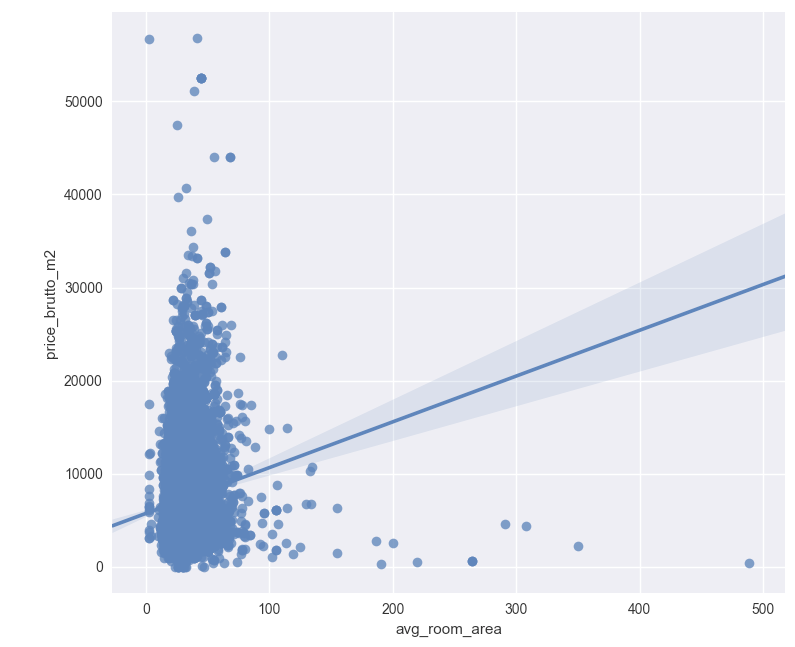
\includegraphics[width=\linewidth]{images/anhang/analysis/Raum_zu_Preis.png}
    \caption{Raum zu Preis} 
  \end{subfigure}
  \begin{subfigure}{.5\textwidth}
    \centering
    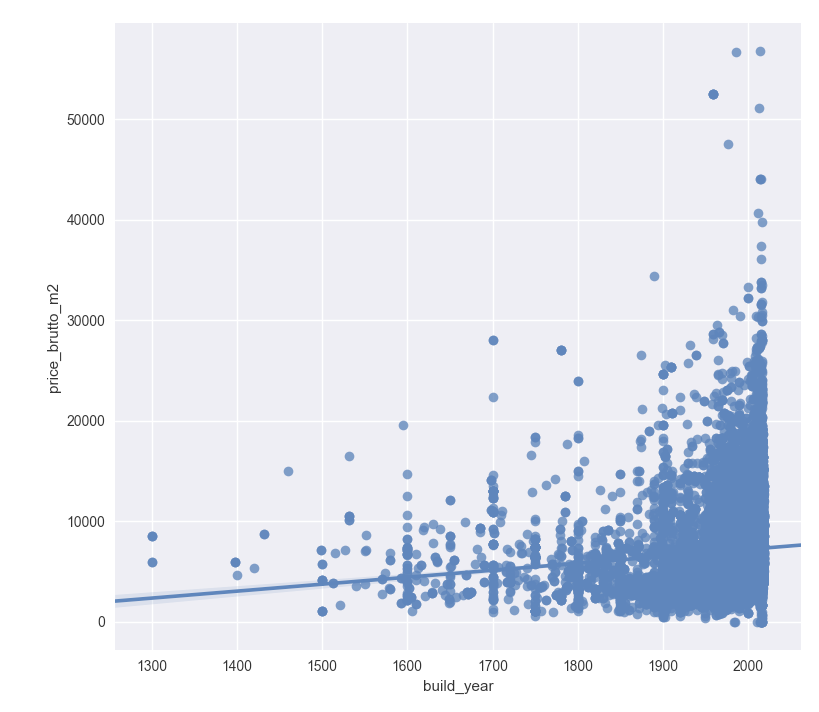
\includegraphics[width=\linewidth]{images/anhang/analysis/BYear_zu_preis.png}
    \caption{Baujahr zu Preis} 
  \end{subfigure}
  \caption{Nummerische Features zum Preis}
  \end{figure}


% - - - - - - - - - - - - - - - - - 
% OUTLIER DETECTION
% - - - - - - - - - - - - - - - - - 
\clearpage
\subsection{Outlier Detection}
Im folgenden werden die Oultiers Detecion Diagramme angezeigt.
\begin{figure}[H]
\begin{subfigure}{.5\textwidth}
\centering
  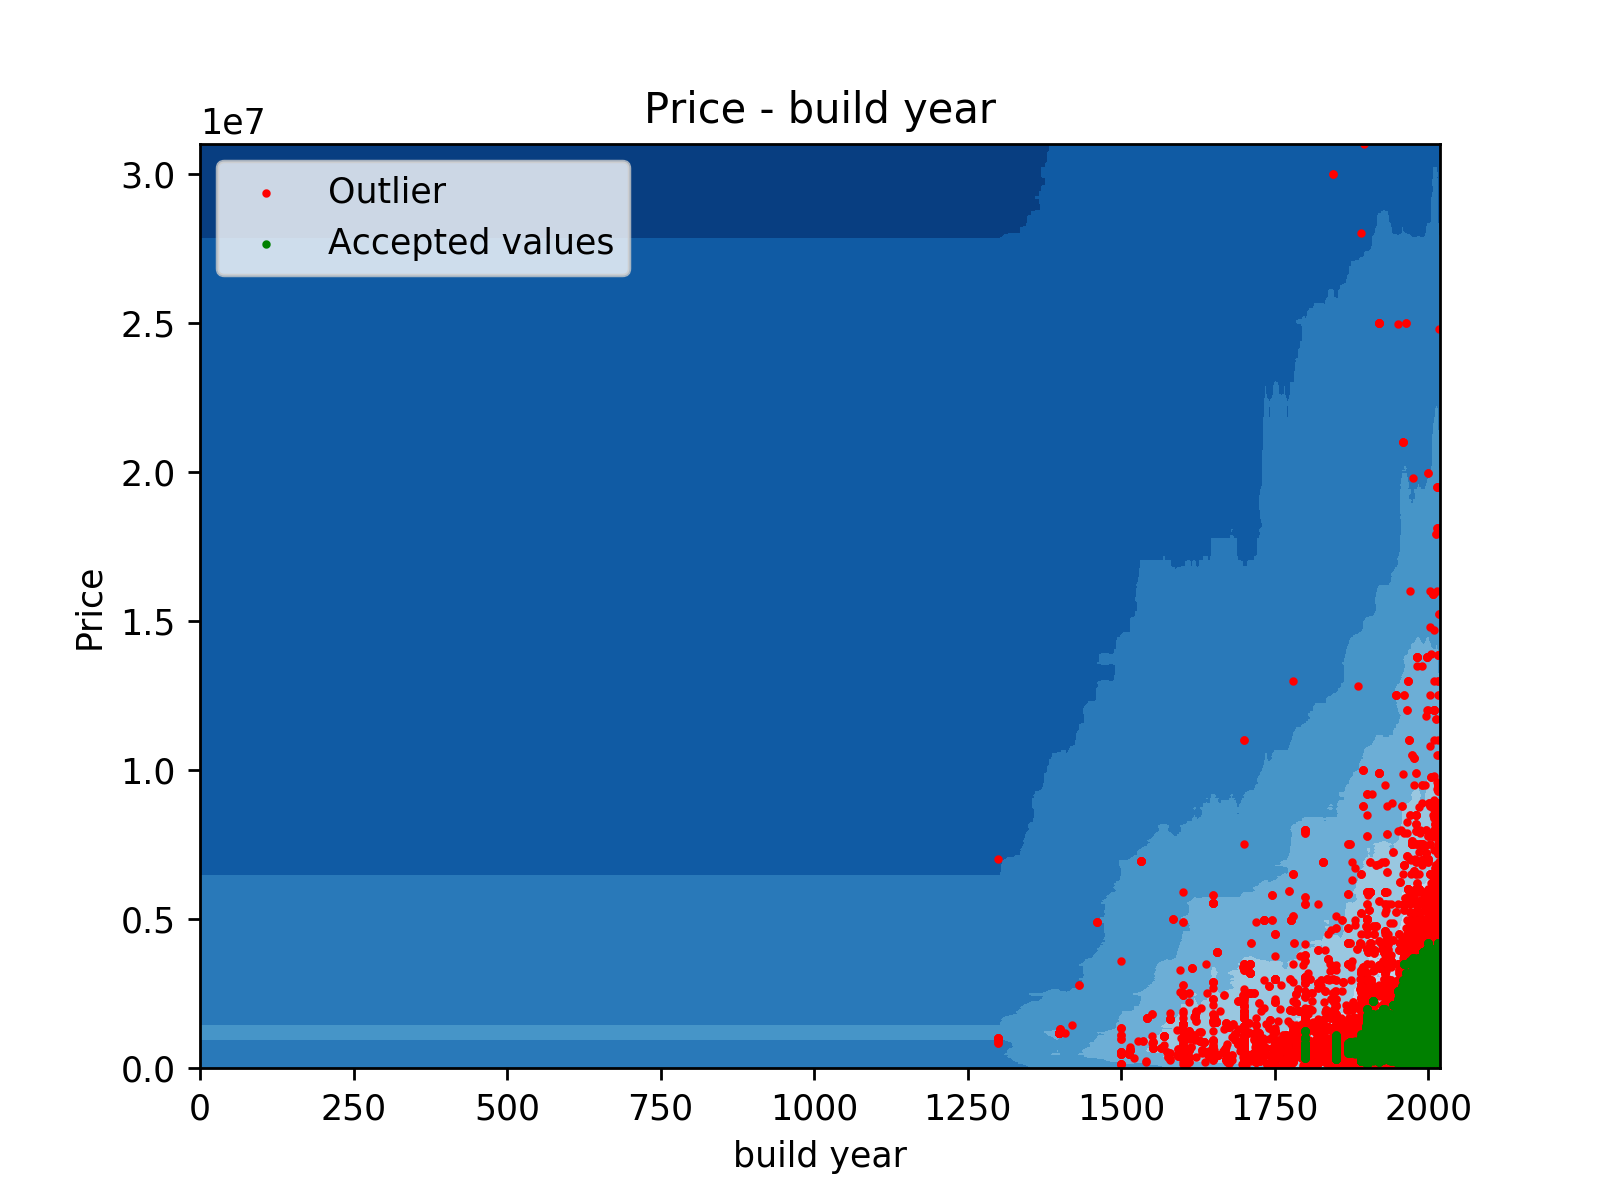
\includegraphics[width=\linewidth]{images/anhang/outlier_detection/build_year_IsolationForest.png}
  \caption{Isolation Forest}
\end{subfigure}
\begin{subfigure}{.5\textwidth}
  \centering
  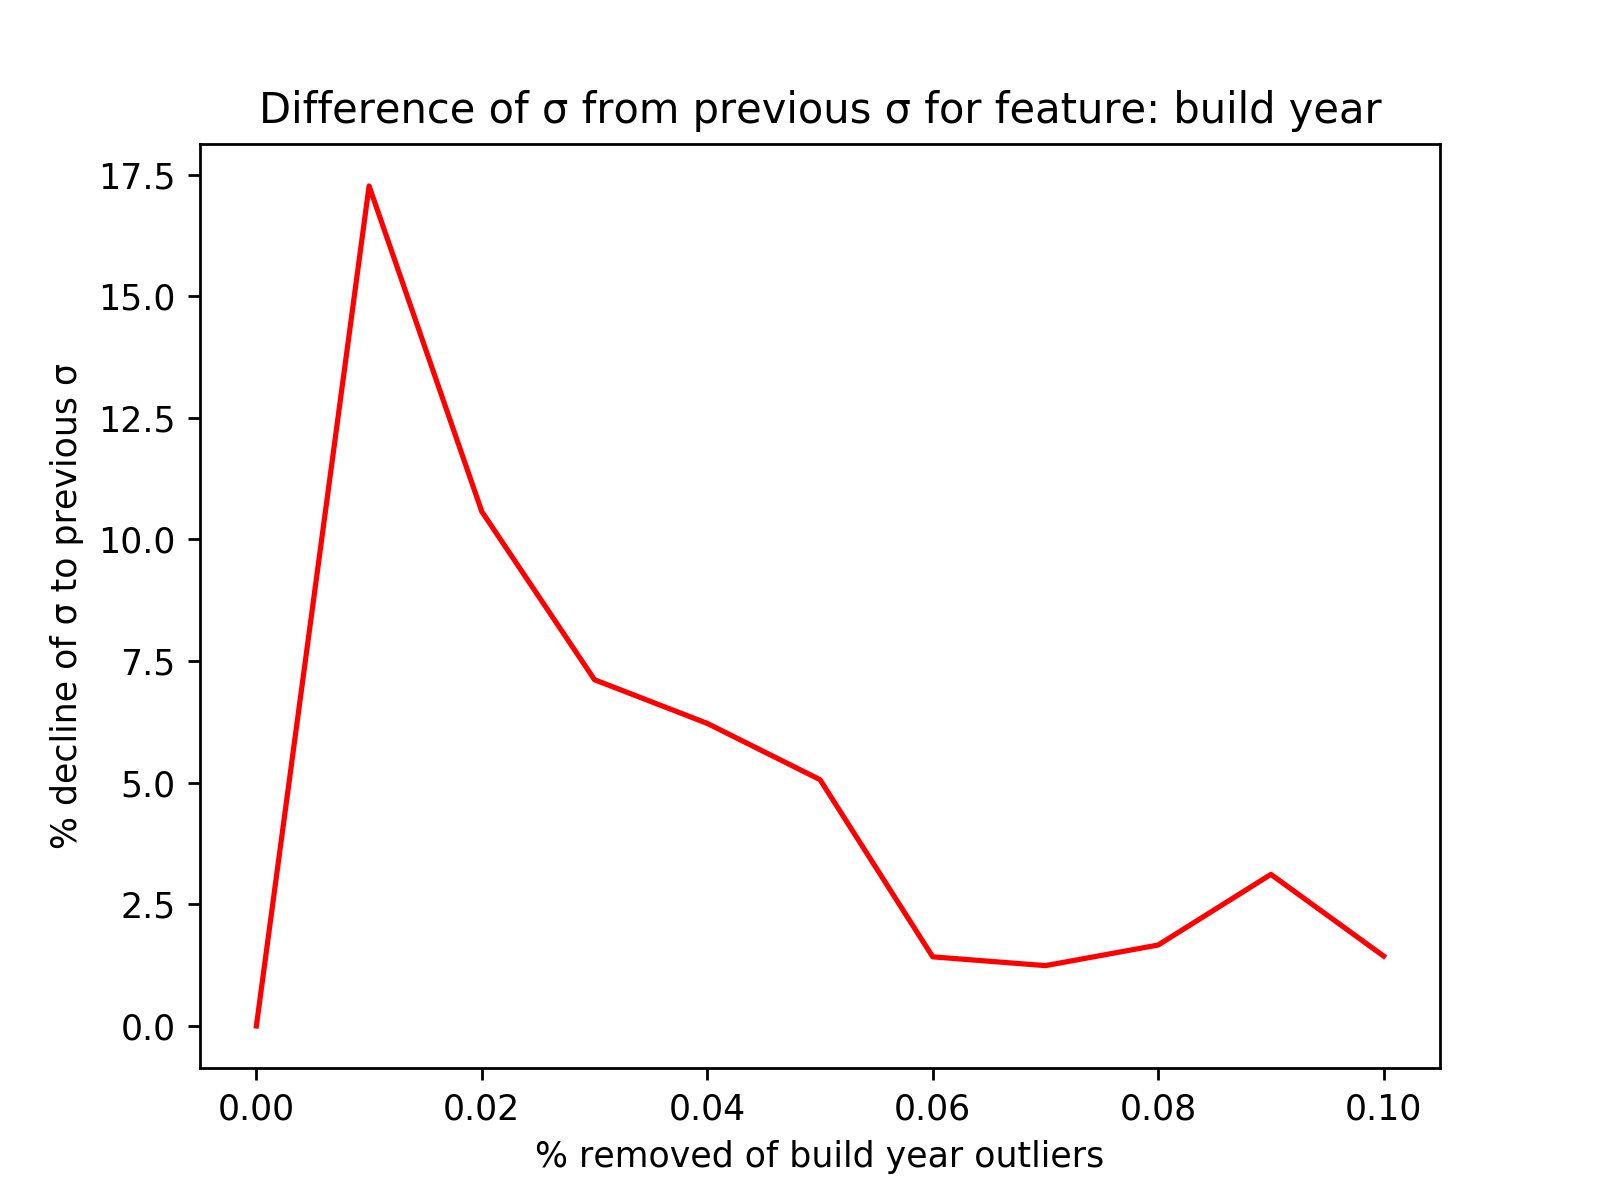
\includegraphics[width=\linewidth]{images/anhang/outlier_detection/build_year_diff_of_std.png}
  \caption{Differenz der Standardabweichug} 
\end{subfigure}
\begin{subfigure}{.5\textwidth}
  \centering
  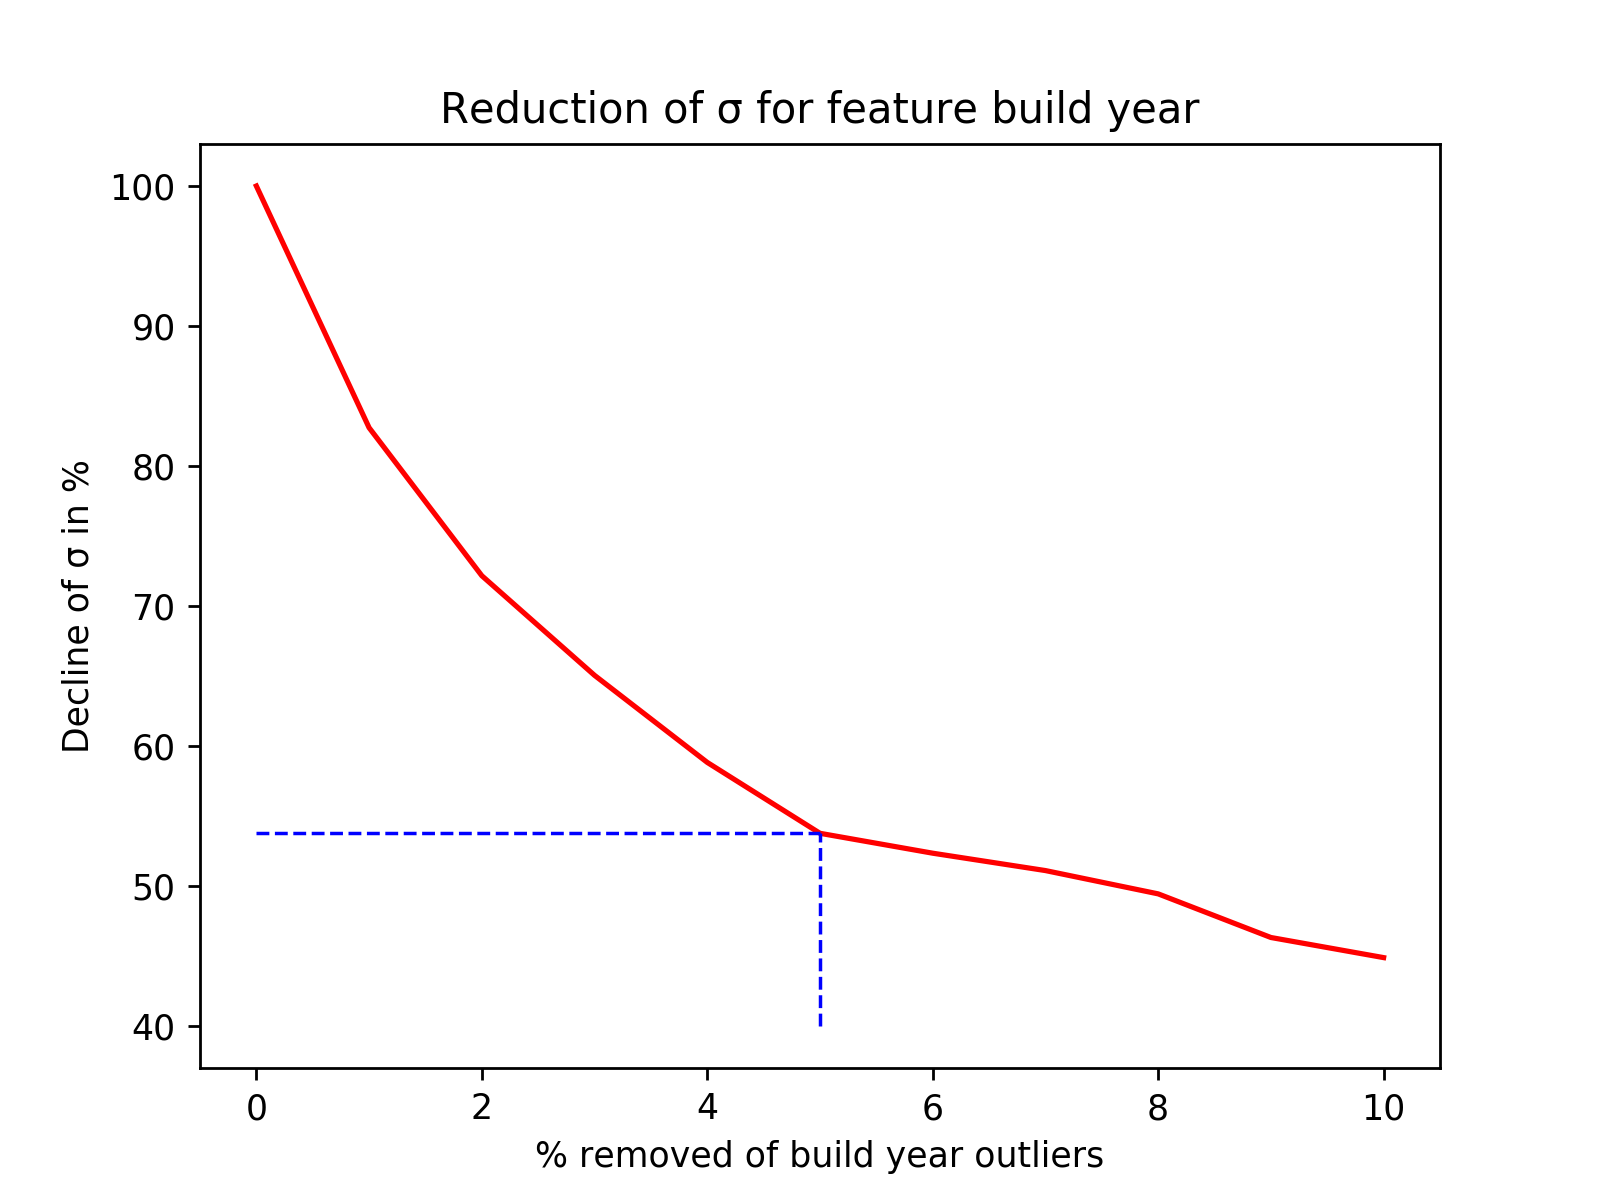
\includegraphics[width=\linewidth]{images/anhang/outlier_detection/build_year_std.png}
  \caption{Veränderung der Standardabweichung} 
\end{subfigure}
\begin{subfigure}{.5\textwidth}
  \centering
  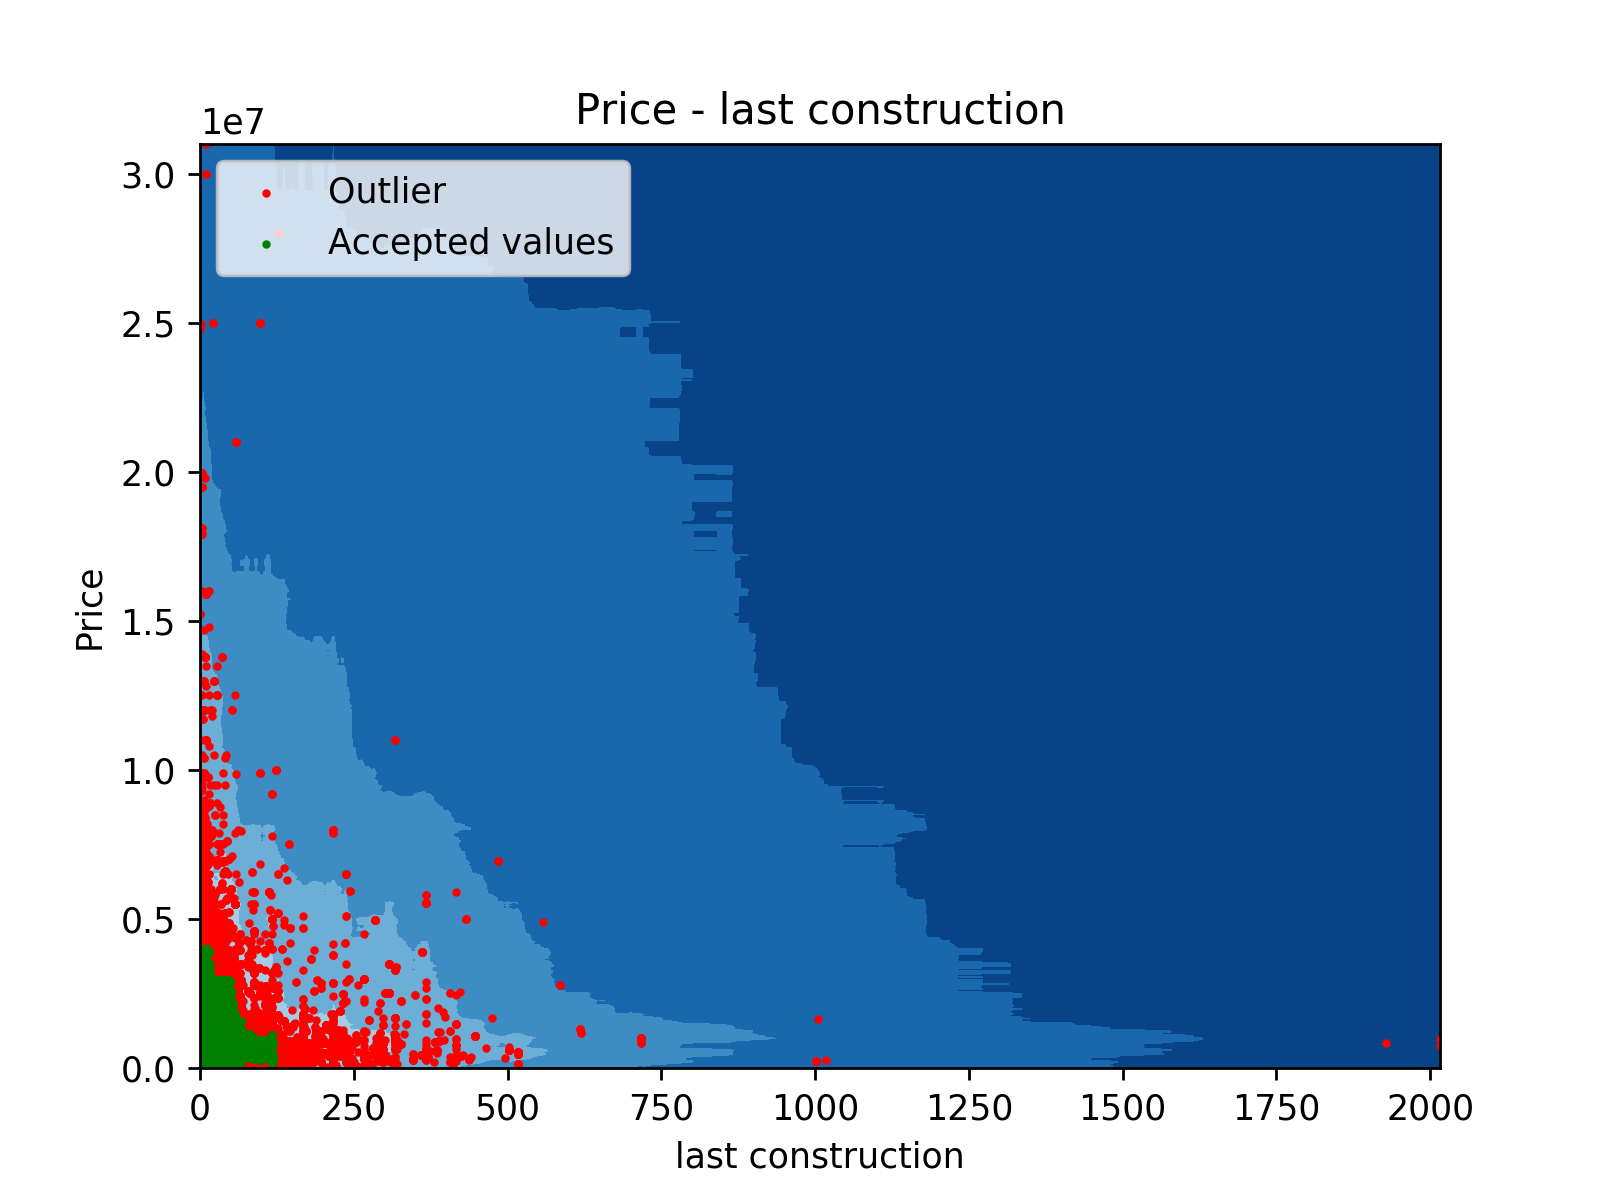
\includegraphics[width=\linewidth]{images/anhang/outlier_detection/last_construction_IsolationForest.png}
  \caption{Isolation Forest}
\end{subfigure}
\begin{subfigure}{.5\textwidth}
  \centering
  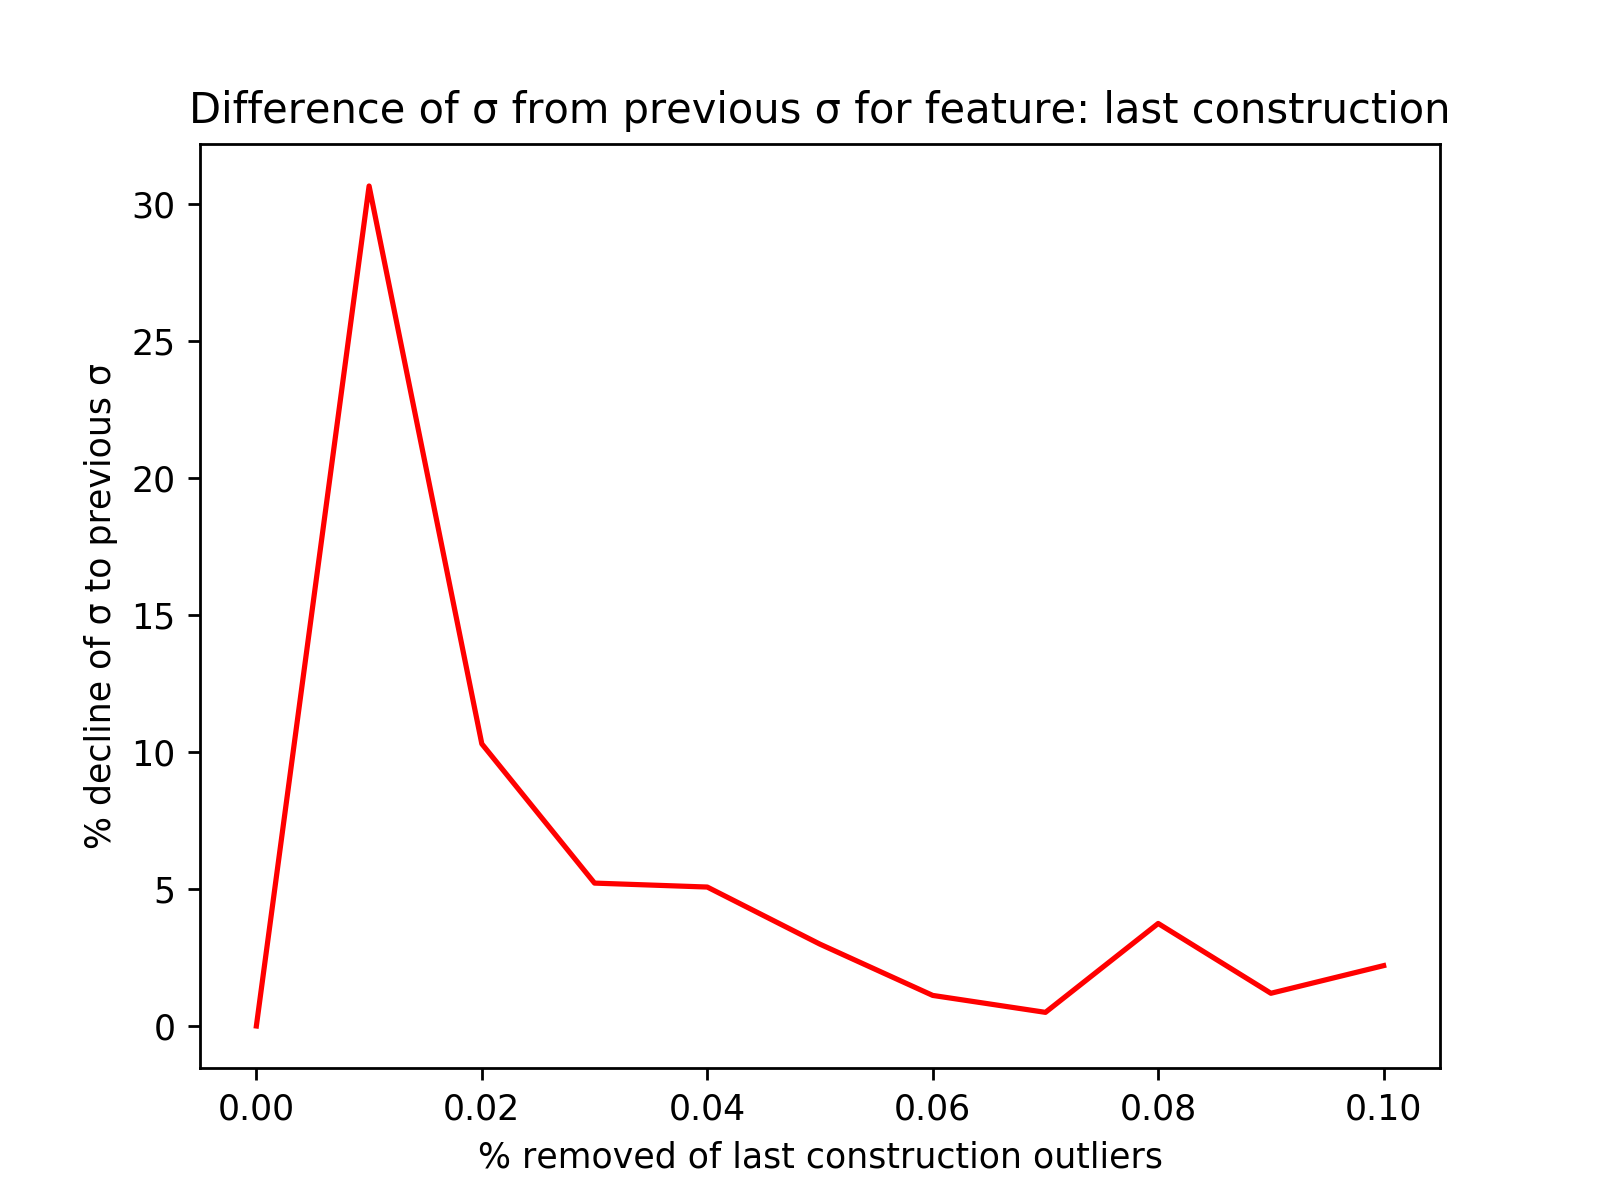
\includegraphics[width=\linewidth]{images/anhang/outlier_detection/last_construction_diff_of_std.png}
  \caption{Differenz der Standardabweichug} 
\end{subfigure}
\begin{subfigure}{.5\textwidth}
  \centering
  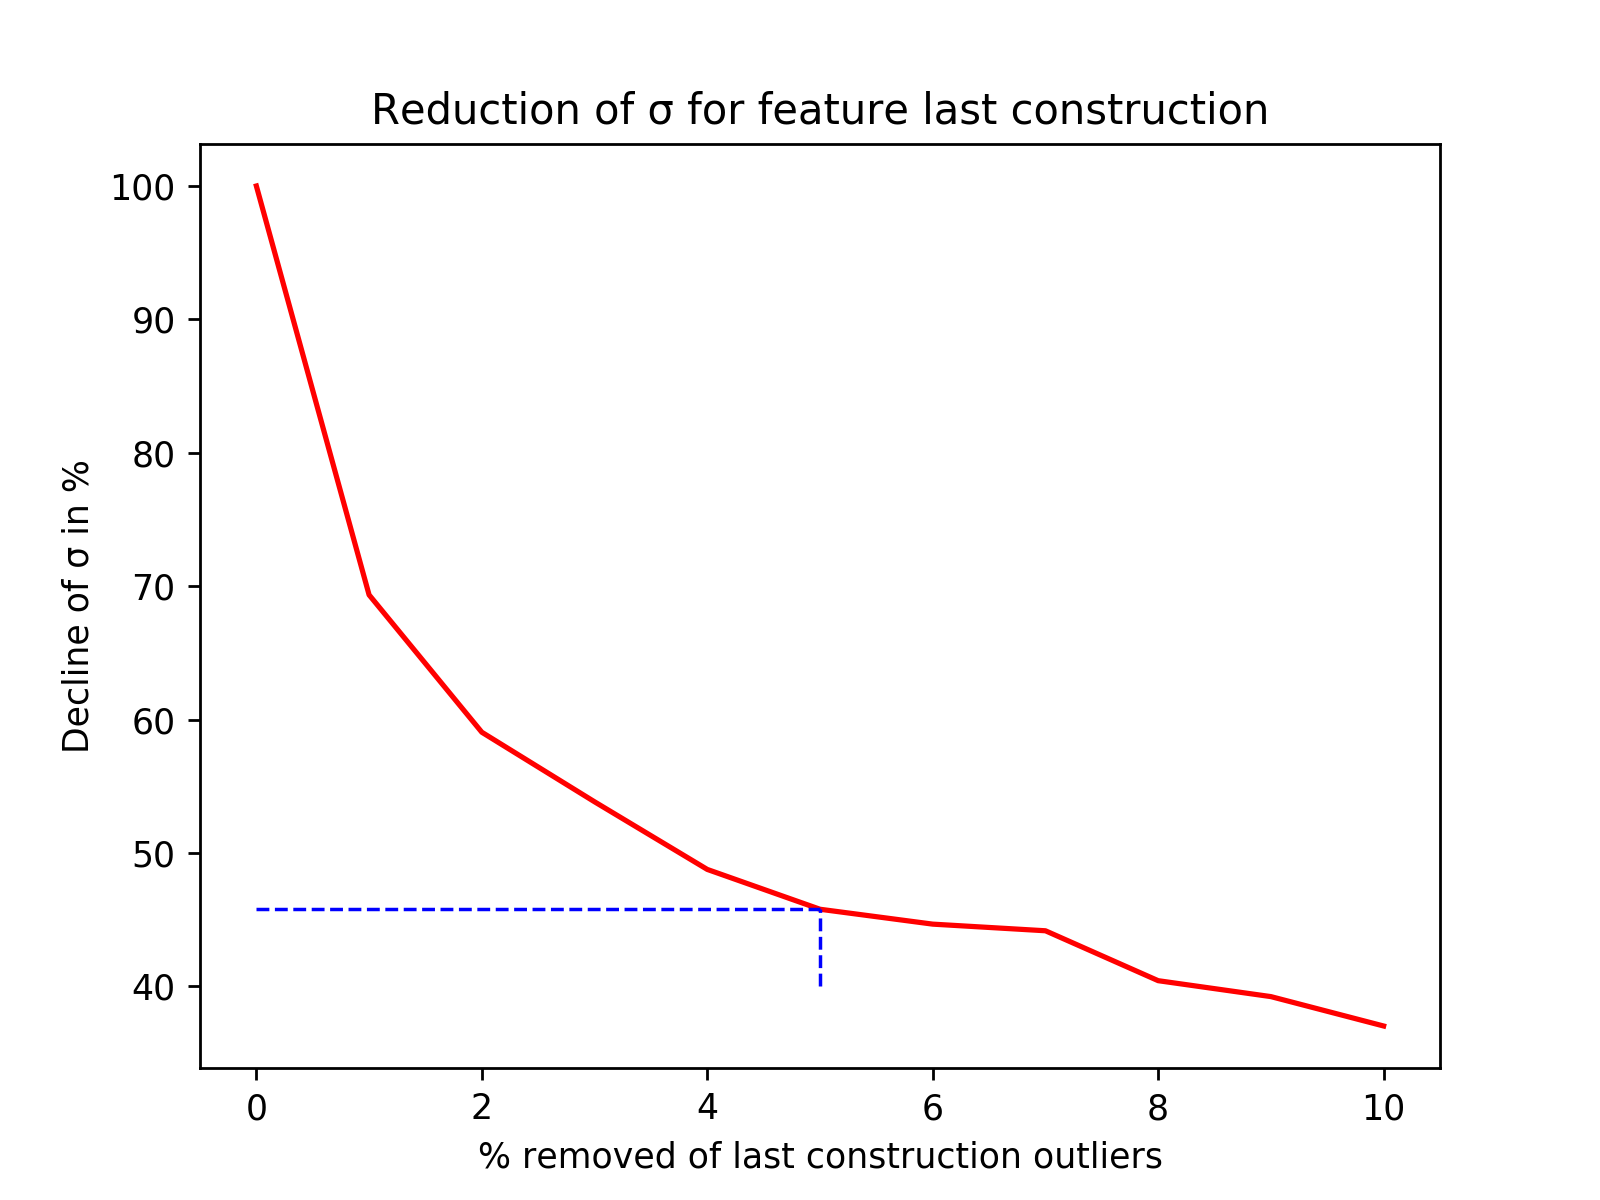
\includegraphics[width=\linewidth]{images/anhang/outlier_detection/last_construction_std.png}
  \caption{Veränderung der Standardabweichung} 
\end{subfigure}
\end{figure}

\begin{figure}[h]
\begin{subfigure}{.5\textwidth}
  \centering
  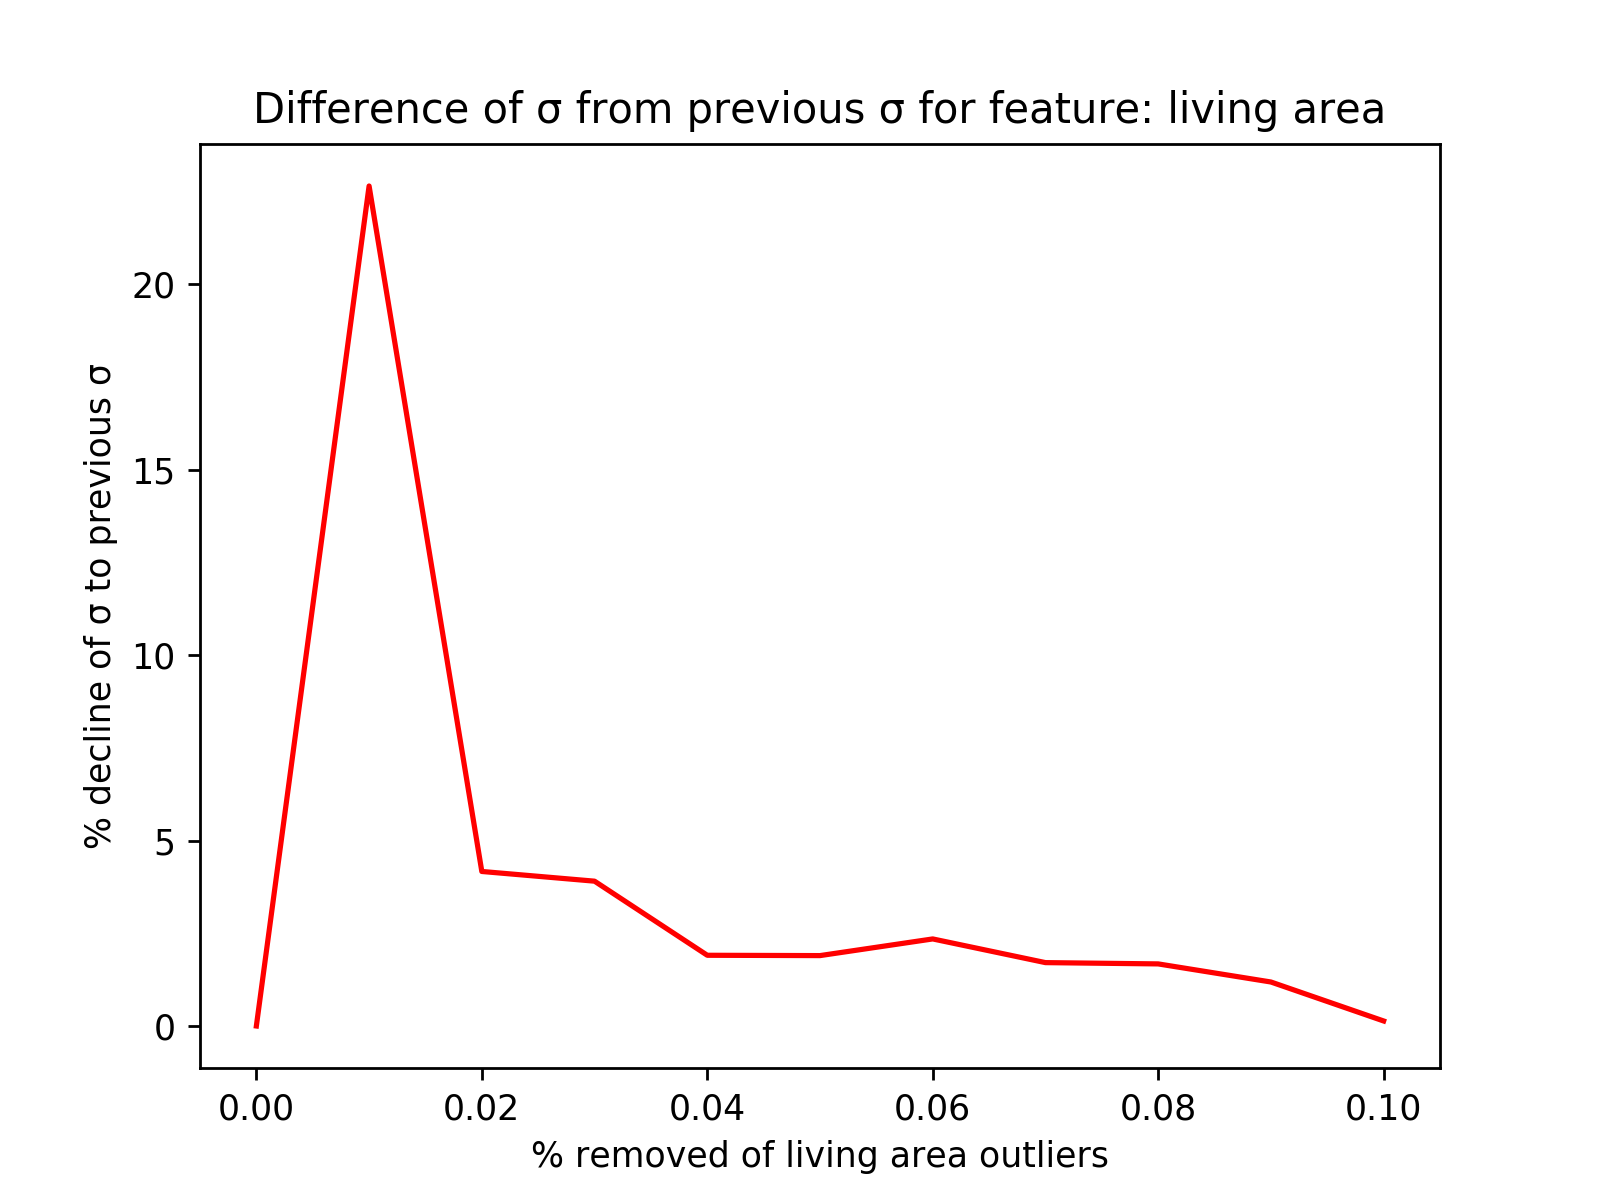
\includegraphics[width=\linewidth]{images/anhang/outlier_detection/living_area_diff_of_std.png}
  \caption{Differenz der Standardabweichung} 
\end{subfigure}
\begin{subfigure}{.5\textwidth}
  \centering
  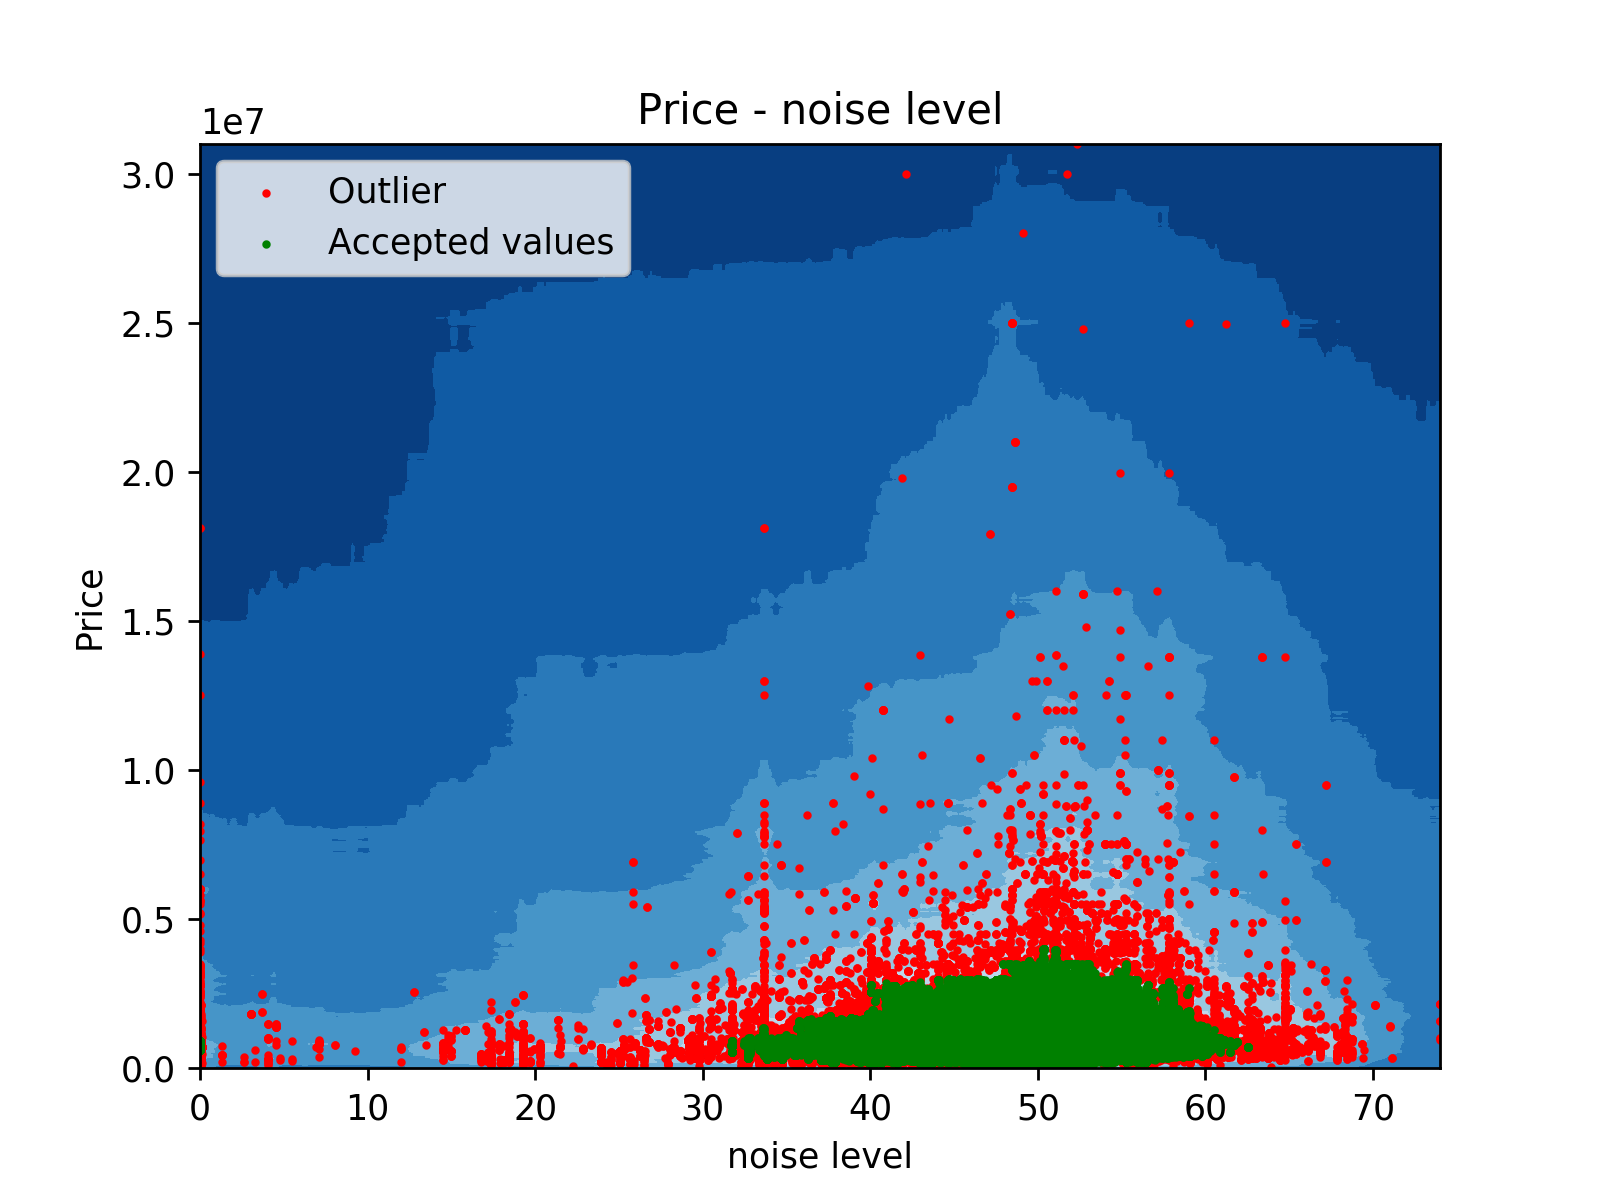
\includegraphics[width=\linewidth]{images/anhang/outlier_detection/noise_level_IsolationForest.png}
  \caption{Isolation Forest} 
\end{subfigure}
\begin{subfigure}{.5\textwidth}
\centering
  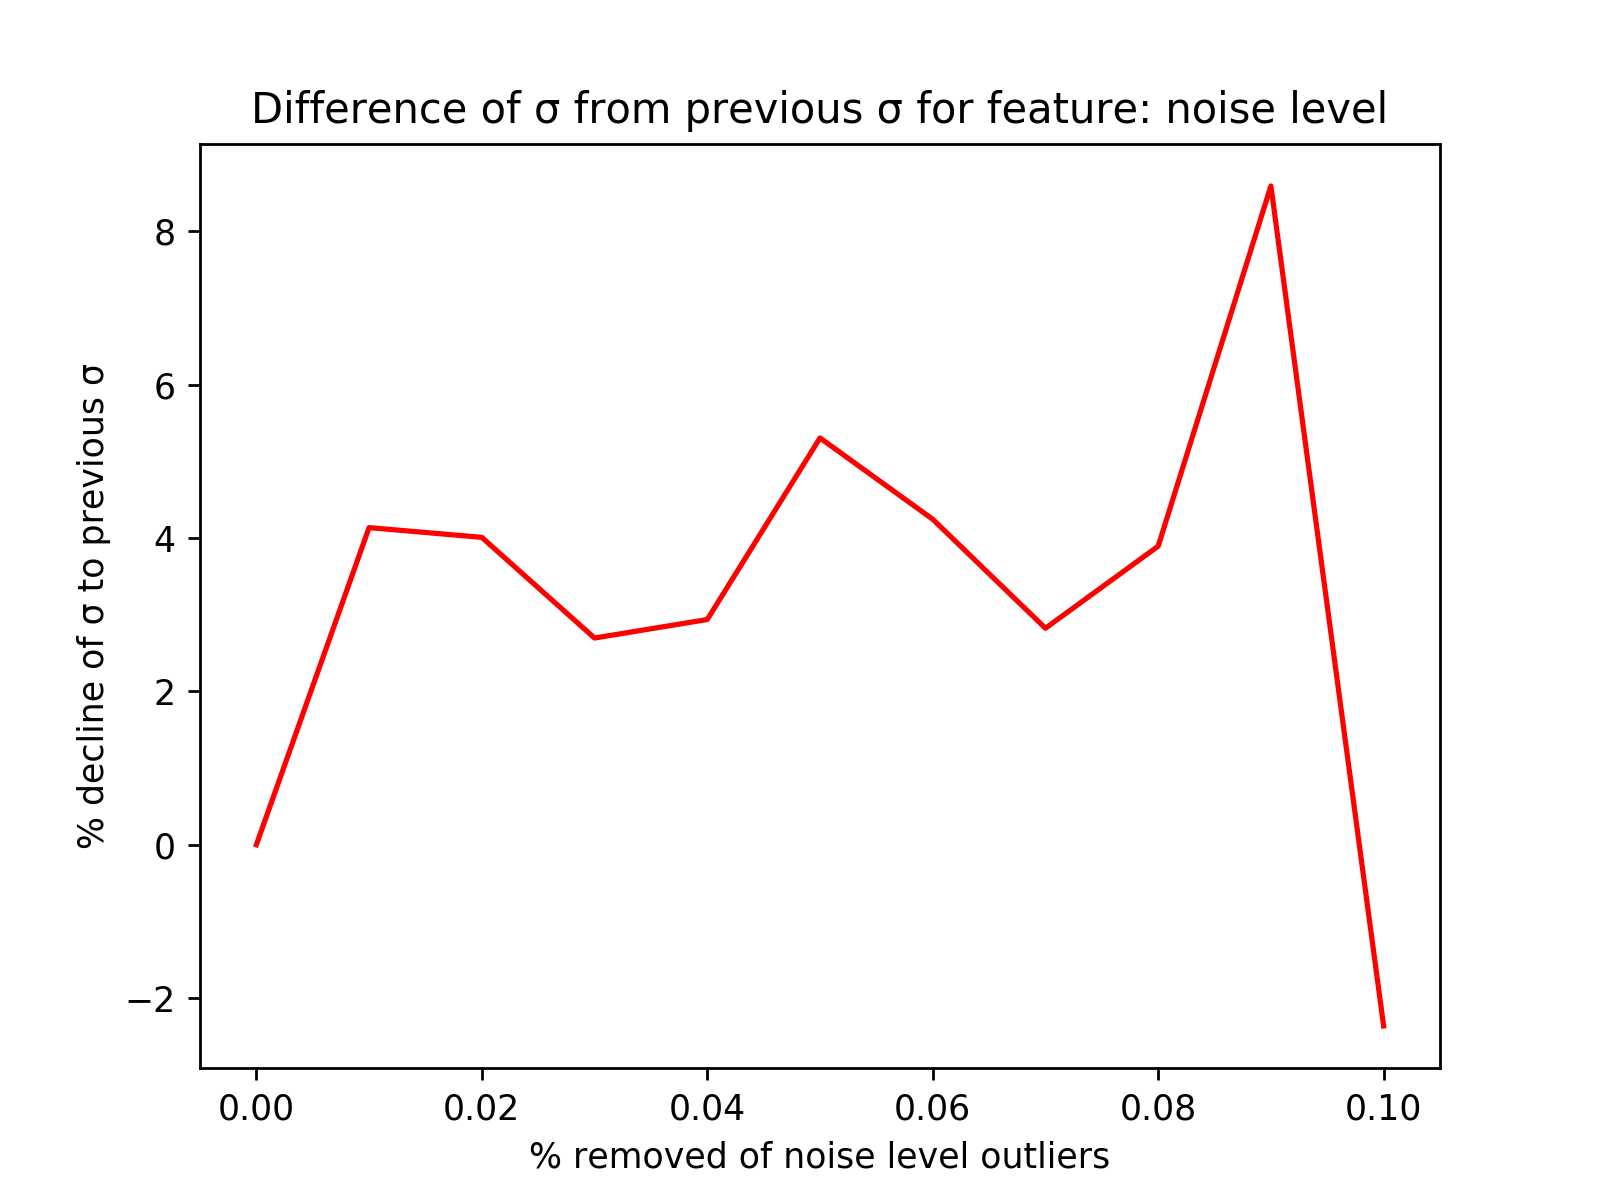
\includegraphics[width=\linewidth]{images/anhang/outlier_detection/noise_level_diff_of_std.png}
  \caption{Differenz der Standardabweichung}
\end{subfigure}
\begin{subfigure}{.5\textwidth}
  \centering
  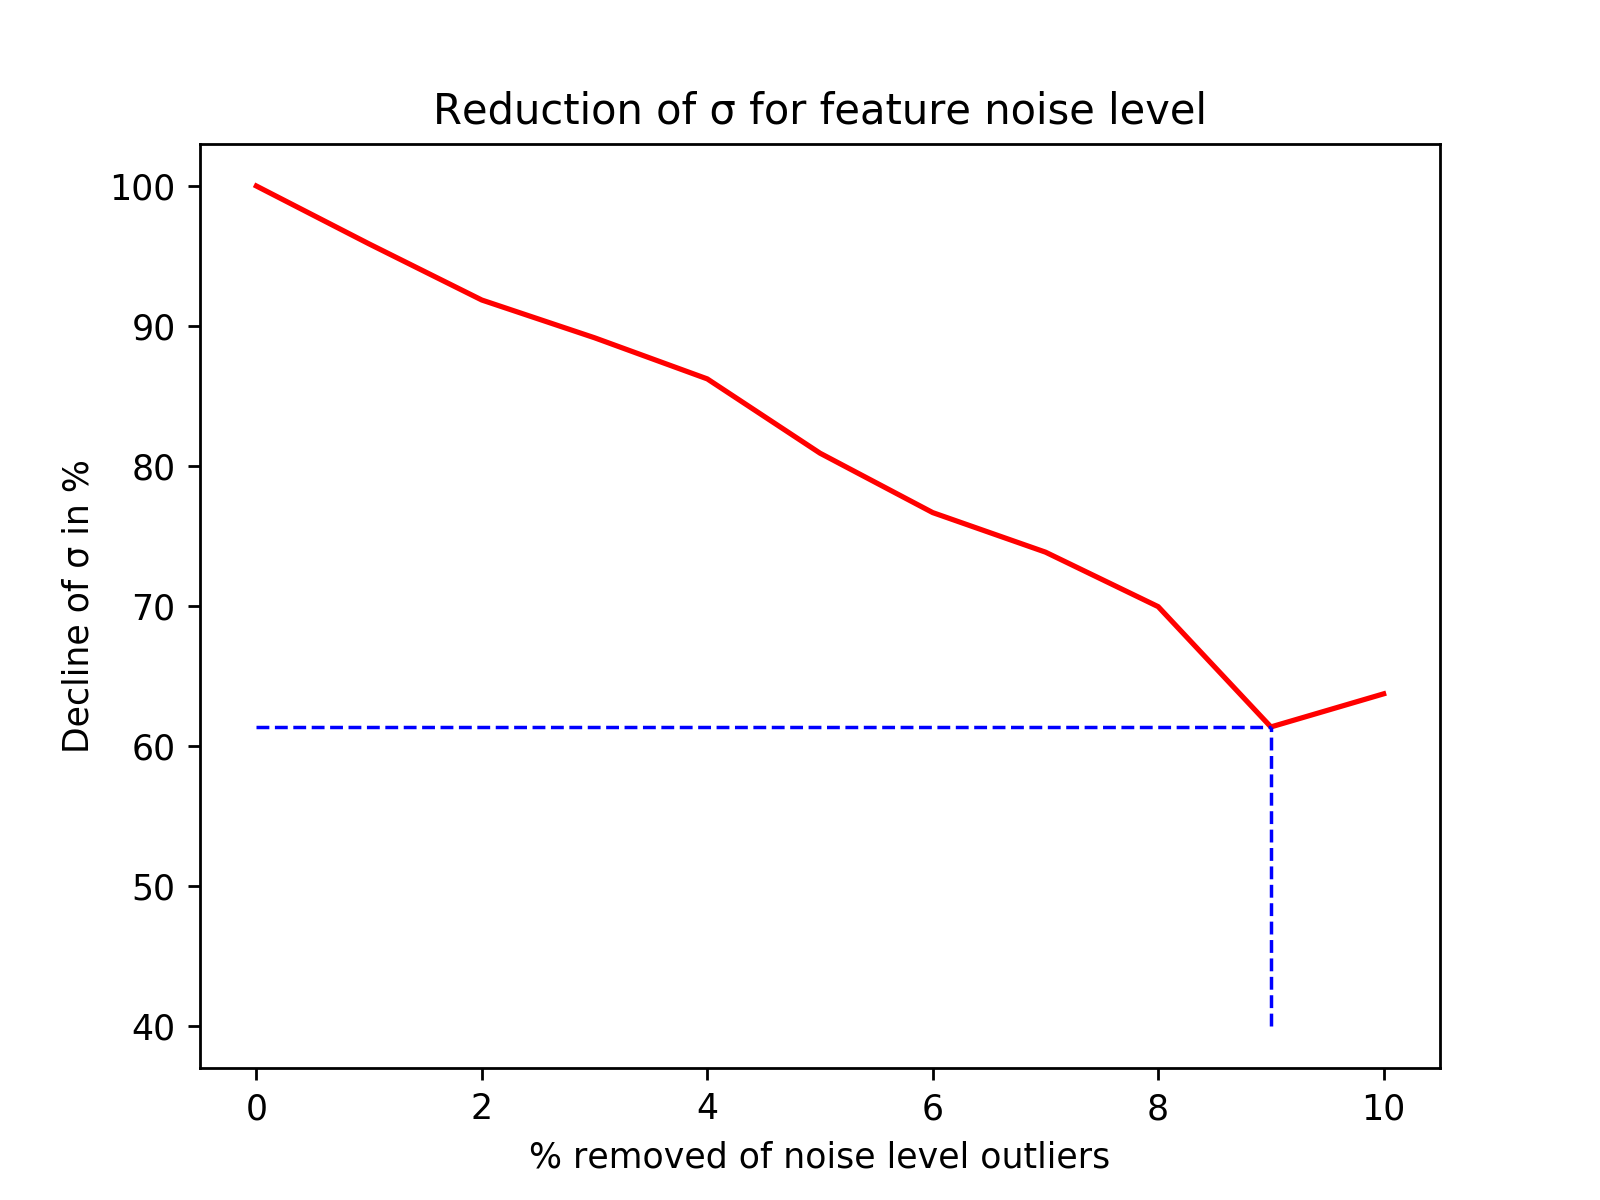
\includegraphics[width=\linewidth]{images/anhang/outlier_detection/noise_level_std.png}
  \caption{Veränderung der Standardabweichung} 
\end{subfigure}
\begin{subfigure}{.5\textwidth}
  \centering
  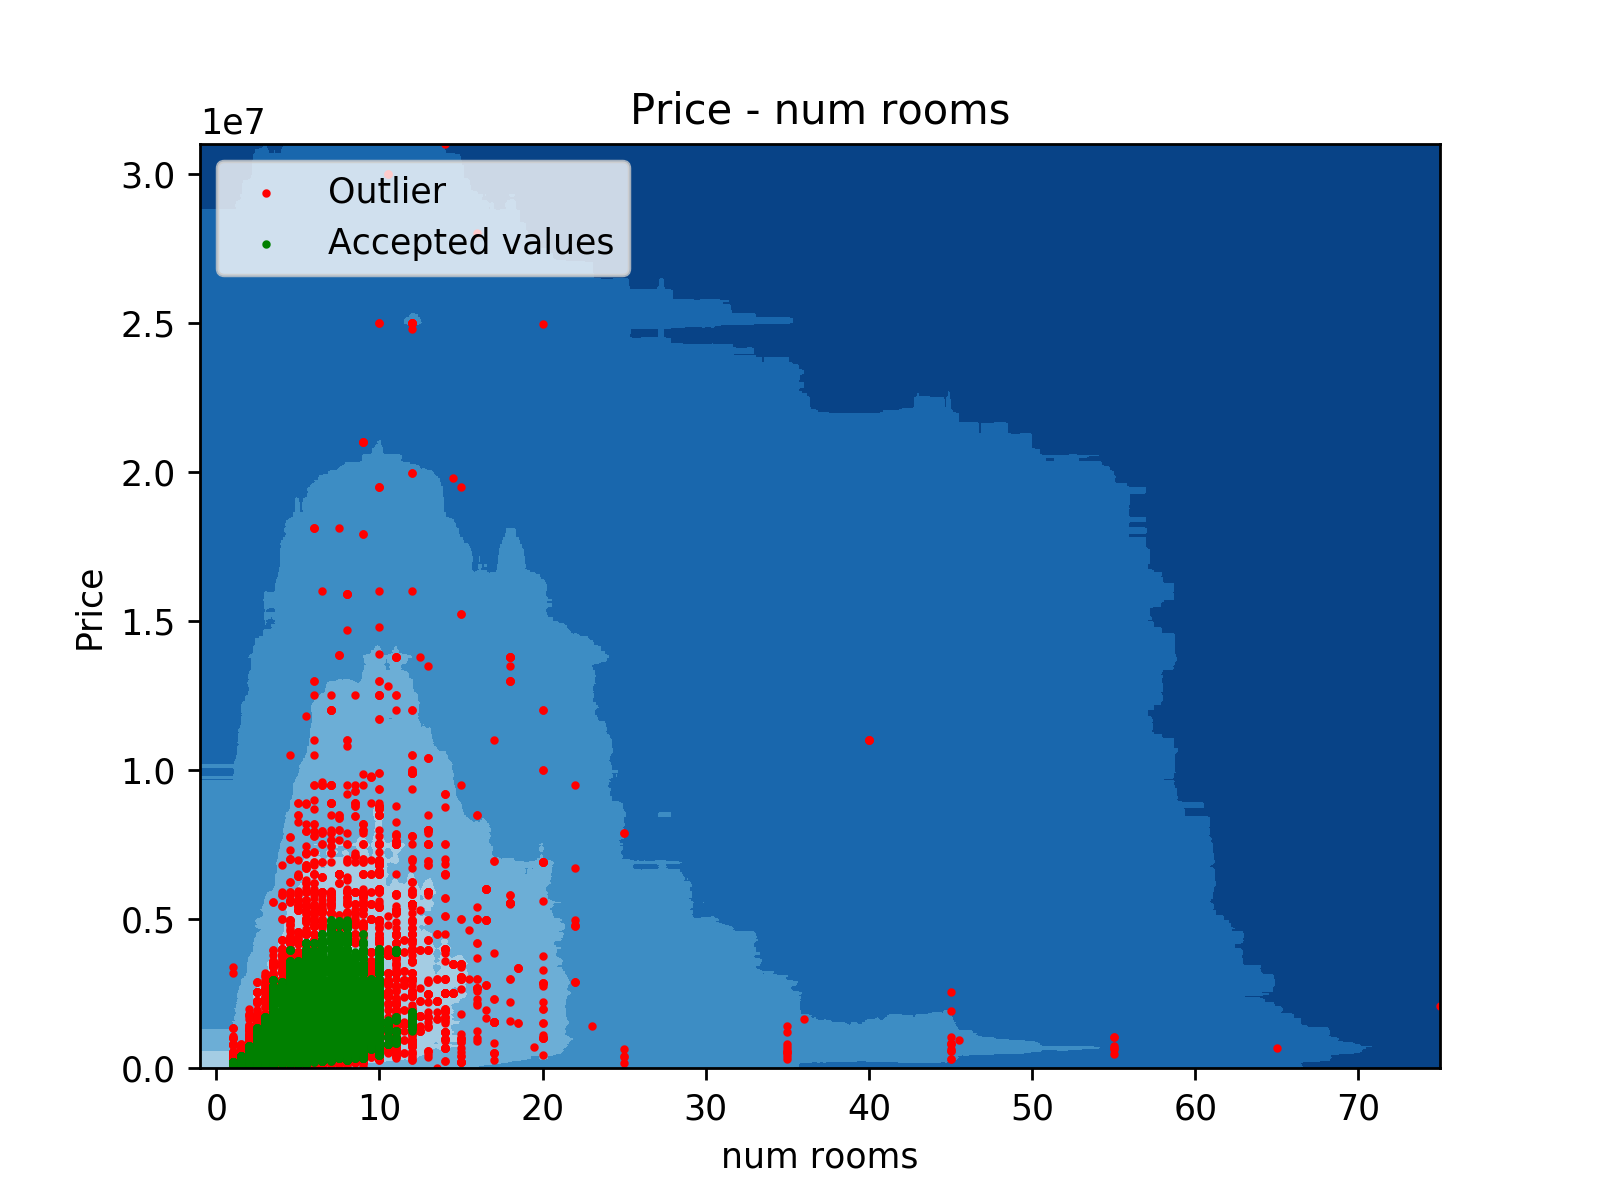
\includegraphics[width=\linewidth]{images/anhang/outlier_detection/num_rooms_IsolationForest.png}
  \caption{Isolation Forest} 
\end{subfigure}
\begin{subfigure}{.5\textwidth}
  \centering
  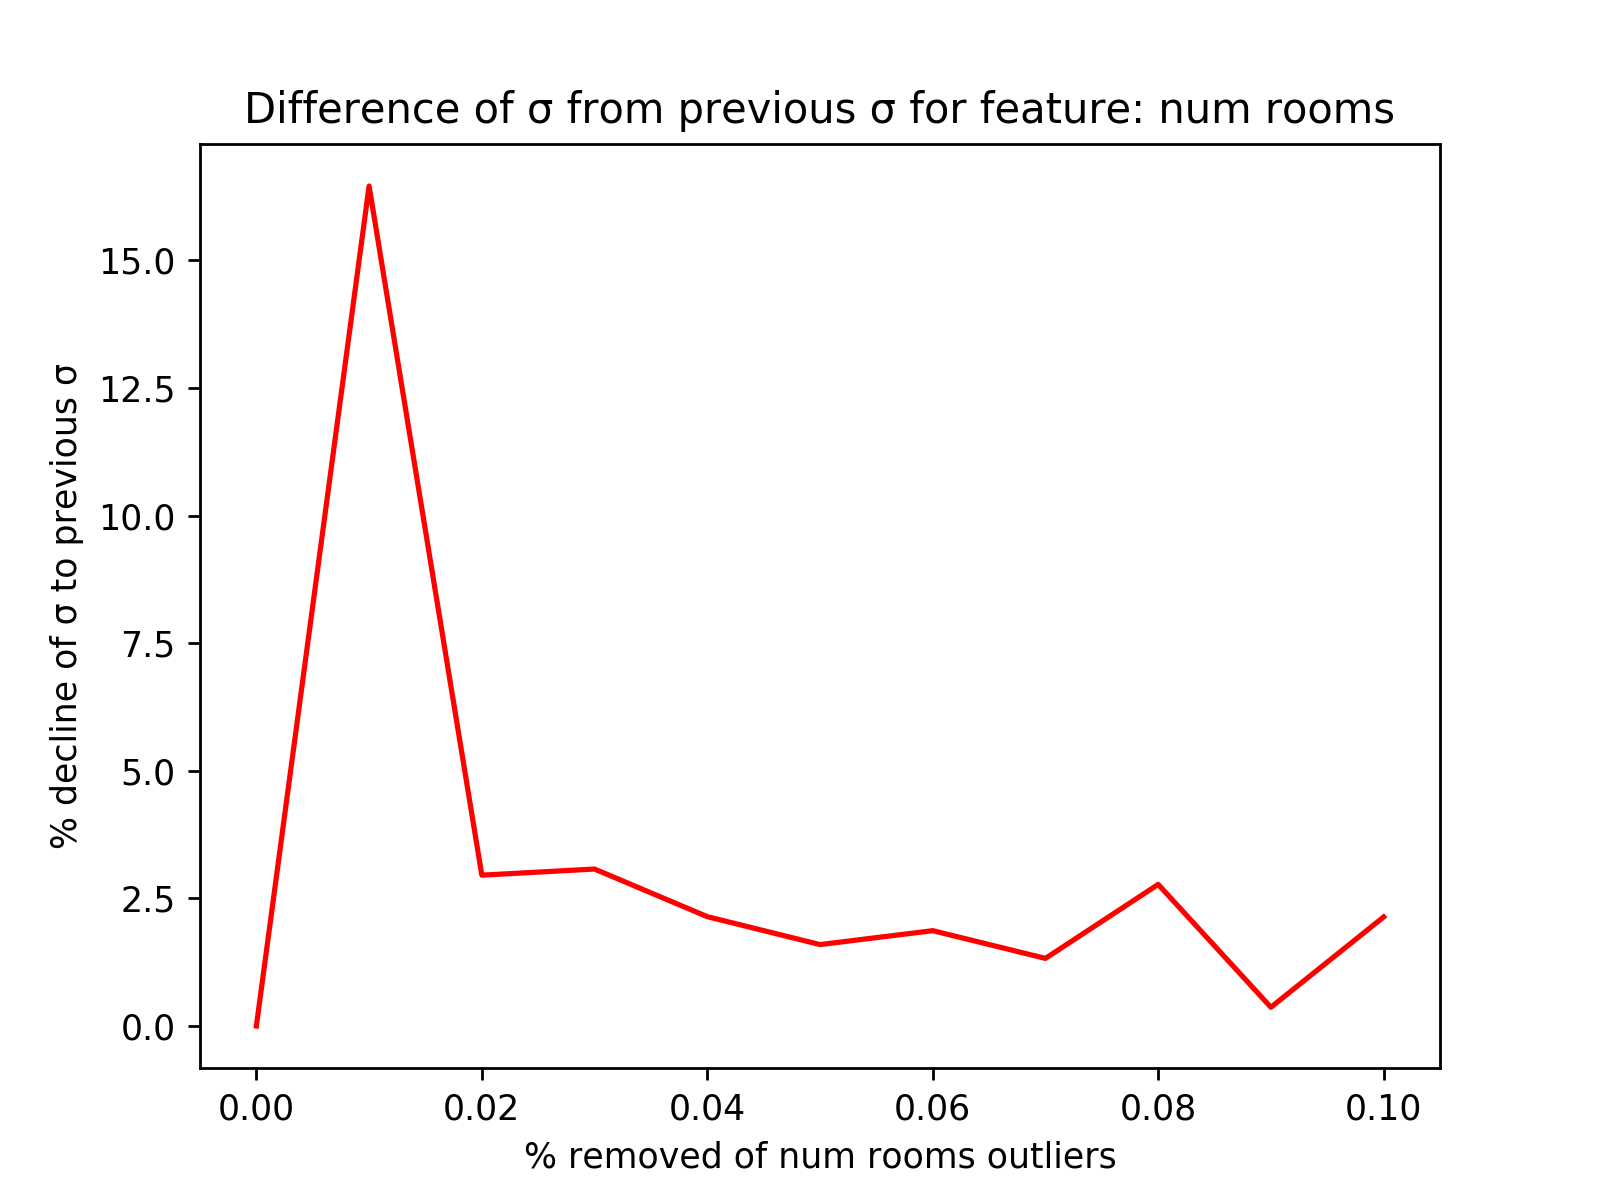
\includegraphics[width=\linewidth]{images/anhang/outlier_detection/num_rooms_diff_of_std.png}
  \caption{Differenz der Standardabweichung} 
\end{subfigure}
\begin{subfigure}{.5\textwidth}
  \centering
  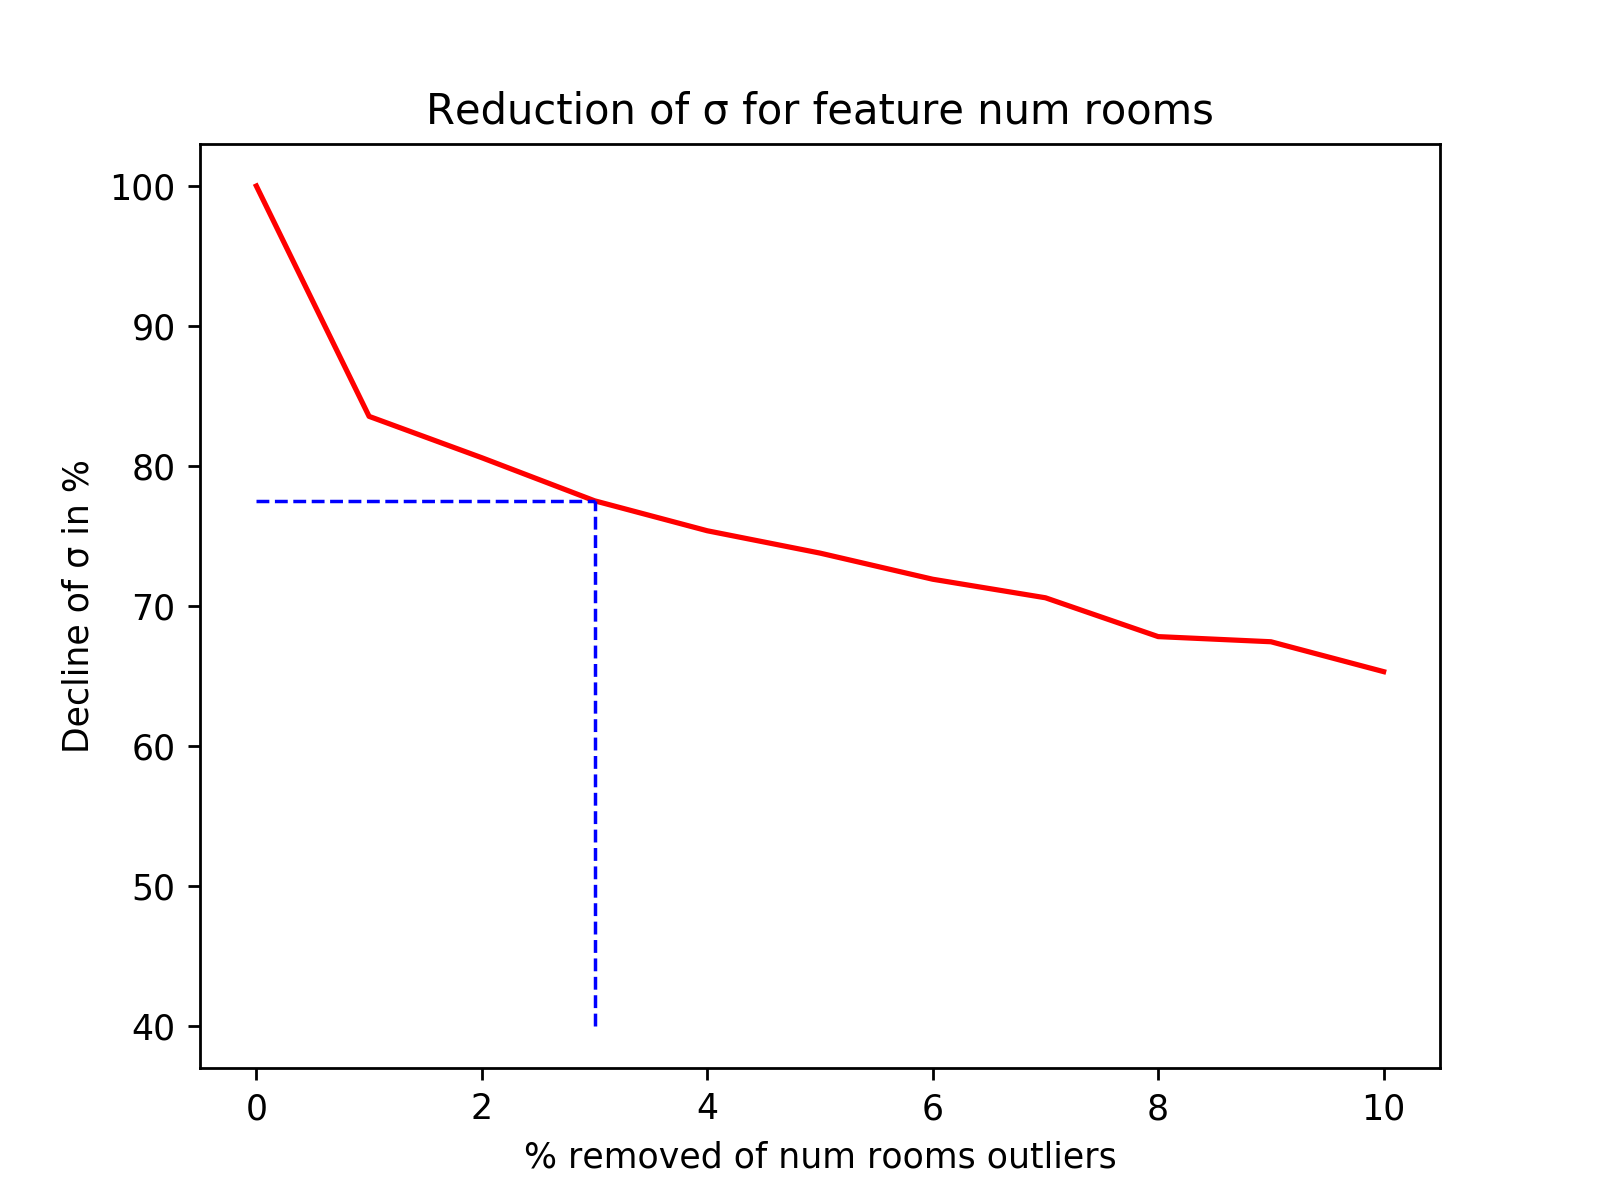
\includegraphics[width=\linewidth]{images/anhang/outlier_detection/num_rooms_std.png}
  \caption{Veränderung der Standardabweichung} 
\end{subfigure}
\caption{Outlier Detection 2}
\end{figure}

% - - - - - - - - - - - - - - - - - 
% Machine Learning
% - - - - - - - - - - - - - - - - - 
\clearpage
\subsection{Machine Learning Resultate}
Im folgenden Abschnitt werden die Performancestatistiken der einezlnen Algorithmen dargestellt.\\[2ex]
\textbf{Lineare Regressions Algorithmen}\\
Performance


\begin{table*}[ht]
\begin{minipage}{.3\textwidth}
\centering
\ra{1.3}
\resizebox{\textwidth}{!}{
\begin{tabular}{@{}lr@{}}
\toprule
Name & Wert in \\
\midrule
            R²-Score & -90633499999999995655749632.00\\
            MAPE & 72553347918093.03\\
            MdAPE & 21.20\\
            Min error & 0.00\\
            Max error & 580978000000000000000.00\\
            Max error  & 6180620000000000.00\\
            Mean absolute error & 385049000000000000.00\\
            Median absolute error & 178672.00\\
            Mean squared error & 100937999999999990998132526851492413440.00\\
\bottomrule
\end{tabular}}
\caption{Linear Regression}
\end{minipage}
\begin{minipage}{.3\textwidth}
\centering
\ra{1.3}
\resizebox{\textwidth}{!}{
\begin{tabular}{@{}lr@{}}
\toprule
Name & Wert in \\
\midrule
            R²-Score & 0.40\\
            MAPE & 79.07\\
            MdAPE & 28.79\\
            Min error & 95.47\\
            Max error & 22248600.00\\
            Max error  & 1618.15\\
            Mean absolute error & 368023.00\\
            Median absolute error & 243025.00\\
            Mean squared error & 564059000000.00\\
\bottomrule
\end{tabular}}
\caption{Ridge}
\end{minipage}
\begin{minipage}{.3\textwidth}
\centering
\ra{1.3}
\resizebox{\textwidth}{!}{
\begin{tabular}{@{}lr@{}}
\toprule
Name & Wert in \\
\midrule
            R²-Score & 0.58\\
            MAPE & 70.04\\
            MdAPE & 19.46\\
            Min error & 16.82\\
            Max error & 27083700.00\\
            Max error  & 1772.81\\
            Mean absolute error & 284884.00\\
            Median absolute error & 161905.00\\
            Mean squared error & 433260000000.00\\
\bottomrule
\end{tabular}}
\caption{Lasso}
\end{minipage}
\end{table*}
                
Abdeckung der Inserate mit Testdaten


\begin{table*}[ht]
\begin{minipage}{.3\textwidth}
\centering
\ra{1.3}
\resizebox{\textwidth}{!}{
\begin{tabular}{@{}lr@{}}
\toprule
Abweichung in \% & Abdeckung in \%\\
\midrule
5 & 13.14\\
10 & 25.93\\
15 & 37.77\\
20 & 47.83\\
25 & 56.47\\
30 & 63.92\\
35 & 69.78\\
40 & 74.66\\
45 & 78.72\\
50 & 81.74\\
55 & 84.13\\
60 & 86.15\\
65 & 87.97\\
70 & 89.49\\
75 & 90.70\\
80 & 91.64\\
85 & 92.52\\
90 & 93.23\\
95 & 93.86\\
\bottomrule
\end{tabular}}
\caption{Linear}
\end{minipage}
\begin{minipage}{.3\textwidth}
\centering
\ra{1.3}
\resizebox{\textwidth}{!}{
\begin{tabular}{@{}lr@{}}
\toprule
Abweichung in \% & Abdeckung in \%\\
\midrule
5 & 9.56\\
10 & 18.62\\
15 & 27.59\\
20 & 36.01\\
25 & 44.22\\
30 & 51.48\\
35 & 58.04\\
40 & 64.06\\
45 & 69.33\\
50 & 73.15\\
55 & 76.36\\
60 & 78.87\\
65 & 81.48\\
70 & 83.52\\
75 & 85.28\\
80 & 86.61\\
85 & 87.80\\
90 & 88.62\\
95 & 89.63\\
\bottomrule
\end{tabular}}
\caption{Ridge}
\end{minipage}
\begin{minipage}{.3\textwidth}
\centering
\ra{1.3}
\resizebox{\textwidth}{!}{
\begin{tabular}{@{}lr@{}}
\toprule
Abweichung in \% & Abdeckung in \%\\
\midrule
5 & 13.97\\
10 & 27.82\\
15 & 40.17\\
20 & 51.05\\
25 & 60.05\\
30 & 67.83\\
35 & 73.75\\
40 & 77.90\\
45 & 81.48\\
50 & 84.15\\
55 & 86.34\\
60 & 88.05\\
65 & 89.57\\
70 & 90.83\\
75 & 91.92\\
80 & 92.70\\
85 & 93.37\\
90 & 93.92\\
95 & 94.65\\
\bottomrule
\end{tabular}}
\caption{Lasso}
\end{minipage}
\end{table*}

%
\newpage
\textbf{KNN und Random Forest}\\
Performance


\begin{table*}[ht]
\begin{minipage}{.3\textwidth}
\centering
\ra{1.3}
\resizebox{\textwidth}{!}{
\begin{tabular}{@{}lr@{}}
\toprule
Name & Wert in \\
\midrule
            R²-Score & 0.83\\
            MAPE & 23.67\\
            MdAPE & 0.00\\
            Min error & 0.00\\
            Max error & 18116100.00\\
            Max error  & 1066.86\\
            Mean absolute error & 99737.00\\
            Median absolute error & 0.00\\
            Mean squared error & 174652000000.00\\
\bottomrule
\end{tabular}}
\caption{K-Nearest Neighbour}
\end{minipage}
\begin{minipage}{.3\textwidth}
\centering
\ra{1.3}
\resizebox{\textwidth}{!}{
\begin{tabular}{@{}lr@{}}
\toprule
Name & Wert in \\
\midrule
            R²-Score & 0.91\\
            MAPE & 23.32\\
            MdAPE & 2.43\\
            Min error & 0.00\\
            Max error & 12637000.00\\
            Max error  & 1128.56\\
            Mean absolute error & 91672.00\\
            Median absolute error & 19802.80\\
            Mean squared error & 95640800000.00\\
\bottomrule
\end{tabular}}
\caption{Random Forest}
\end{minipage}
\end{table*}
                
Abdeckung der Inserate mit Testdaten


\begin{table*}[ht]
\begin{minipage}{.3\textwidth}
\centering
\ra{1.3}
\resizebox{\textwidth}{!}{
\begin{tabular}{@{}lr@{}}
\toprule
Abweichung in \% & Abdeckung in \%\\
\midrule
5 & 71.28\\
10 & 79.94\\
15 & 84.91\\
20 & 88.02\\
25 & 90.12\\
30 & 91.85\\
35 & 93.26\\
40 & 94.39\\
45 & 95.15\\
50 & 95.86\\
55 & 96.39\\
60 & 96.88\\
65 & 97.25\\
70 & 97.59\\
75 & 97.80\\
80 & 98.03\\
85 & 98.16\\
90 & 98.33\\
95 & 98.49\\
\bottomrule
\end{tabular}}
\caption{K-Nearest Neighbor}
\end{minipage}
\begin{minipage}{.3\textwidth}
\centering
\ra{1.3}
\resizebox{\textwidth}{!}{
\begin{tabular}{@{}lr@{}}
\toprule
Abweichung in \% & Abdeckung in \%\\
\midrule
5 & 63.53\\
10 & 77.52\\
15 & 84.92\\
20 & 89.08\\
25 & 92.12\\
30 & 94.17\\
35 & 95.53\\
40 & 96.52\\
45 & 97.22\\
50 & 97.72\\
55 & 98.15\\
60 & 98.43\\
65 & 98.68\\
70 & 98.85\\
75 & 98.97\\
80 & 99.11\\
85 & 99.19\\
90 & 99.27\\
95 & 99.32\\
\bottomrule
\end{tabular}}
\caption{Random Forest}
\end{minipage}
\end{table*}

%
\newpage
\textbf{Baumalgorithmen}\\
Performance


\begin{table*}[ht]
\begin{minipage}{.3\textwidth}
\centering
\ra{1.3}
\resizebox{\textwidth}{!}{
\begin{tabular}{@{}lr@{}}
\toprule
Name & Wert in \\
\midrule
            R²-Score & 0.90\\
            MAPE & 18.71\\
            MdAPE & 0.81\\
            Min error & 0.00\\
            Max error & 14595700.00\\
            Max error  & 1149.96\\
            Mean absolute error & 77841.60\\
            Median absolute error & 6007.62\\
            Mean squared error & 104216000000.00\\
\bottomrule
\end{tabular}}
\caption{XGBoost}
\end{minipage}
\begin{minipage}{.3\textwidth}
\centering
\ra{1.3}
\resizebox{\textwidth}{!}{
\begin{tabular}{@{}lr@{}}
\toprule
Name & Wert in \\
\midrule
            R²-Score & 0.91\\
            MAPE & 23.88\\
            MdAPE & 0.86\\
            Min error & 0.00\\
            Max error & 10386900.00\\
            Max error  & 1325.92\\
            Mean absolute error & 77036.20\\
            Median absolute error & 6607.14\\
            Mean squared error & 92124700000.00\\
\bottomrule
\end{tabular}}
\caption{Extra Trees}
\end{minipage}
\begin{minipage}{.3\textwidth}
\centering
\ra{1.3}
\resizebox{\textwidth}{!}{
\begin{tabular}{@{}lr@{}}
\toprule
Name & Wert in \\
\midrule
            R²-Score & 0.91\\
            MAPE & 18.14\\
            MdAPE & 0.00\\
            Min error & 0.00\\
            Max error & 16300000.00\\
            Max error  & 1174.47\\
            Mean absolute error & 66601.90\\
            Median absolute error & 0.00\\
            Mean squared error & 95856800000.00\\
\bottomrule
\end{tabular}}
\caption{AdaBoost}
\end{minipage}
\end{table*}
                
Abdeckung der Inserate mit Testdaten


\begin{table*}[ht]
\begin{minipage}{.3\textwidth}
\centering
\ra{1.3}
\resizebox{\textwidth}{!}{
\begin{tabular}{@{}lr@{}}
\toprule
Abweichung in \% & Abdeckung in \%\\
\midrule
5 & 71.52\\
10 & 82.01\\
15 & 87.27\\
20 & 90.65\\
25 & 92.94\\
30 & 94.44\\
35 & 95.60\\
40 & 96.54\\
45 & 97.37\\
50 & 97.78\\
55 & 98.23\\
60 & 98.47\\
65 & 98.69\\
70 & 98.86\\
75 & 99.00\\
80 & 99.12\\
85 & 99.25\\
90 & 99.30\\
95 & 99.36\\
\bottomrule
\end{tabular}}
\caption{XGBoost}
\end{minipage}
\begin{minipage}{.3\textwidth}
\centering
\ra{1.3}
\resizebox{\textwidth}{!}{
\begin{tabular}{@{}lr@{}}
\toprule
Abweichung in \% & Abdeckung in \%\\
\midrule
5 & 71.26\\
10 & 81.73\\
15 & 87.06\\
20 & 90.48\\
25 & 92.92\\
30 & 94.72\\
35 & 96.02\\
40 & 96.85\\
45 & 97.48\\
50 & 97.97\\
55 & 98.35\\
60 & 98.62\\
65 & 98.85\\
70 & 99.00\\
75 & 99.13\\
80 & 99.21\\
85 & 99.27\\
90 & 99.32\\
95 & 99.36\\
\bottomrule
\end{tabular}}
\caption{Extra Trees}
\end{minipage}
\begin{minipage}{.3\textwidth}
\centering
\ra{1.3}
\resizebox{\textwidth}{!}{
\begin{tabular}{@{}lr@{}}
\toprule
Abweichung in \% & Abdeckung in \%\\
\midrule
5 & 76.22\\
10 & 83.69\\
15 & 87.94\\
20 & 91.04\\
25 & 93.26\\
30 & 94.89\\
35 & 96.10\\
40 & 96.89\\
45 & 97.53\\
50 & 98.01\\
55 & 98.44\\
60 & 98.69\\
65 & 98.86\\
70 & 99.05\\
75 & 99.16\\
80 & 99.28\\
85 & 99.35\\
90 & 99.43\\
95 & 99.49\\
\bottomrule
\end{tabular}}
\caption{AdaBoost}
\end{minipage}
\end{table*}
                
%
\newpage
\textbf{Mit durchschnittlicher Zimmergrösse}\\
Performance


\begin{table*}[ht]
\begin{minipage}{.3\textwidth}
\centering
\ra{1.3}
\resizebox{\textwidth}{!}{
\begin{tabular}{@{}lr@{}}
\toprule
Name & Wert in \\
\midrule
            R²-Score & 0.89\\
            MAPE & 25.27\\
            MdAPE & 0.75\\
            Min error & 0.00\\
            Max error & 23029100.00\\
            Max error  & 1405.89\\
            Mean absolute error & 74692.50\\
            Median absolute error & 5412.00\\
            Mean squared error & 109615000000.00\\
\bottomrule
\end{tabular}}
\caption{XGBoost}
\end{minipage}
\begin{minipage}{.3\textwidth}
\centering
\ra{1.3}
\resizebox{\textwidth}{!}{
\begin{tabular}{@{}lr@{}}
\toprule
Name & Wert in \\
\midrule
            R²-Score & 0.90\\
            MAPE & 27.14\\
            MdAPE & 0.82\\
            Min error & 0.00\\
            Max error & 17641700.00\\
            Max error  & 1370.11\\
            Mean absolute error & 73570.60\\
            Median absolute error & 6100.00\\
            Mean squared error & 94514800000.00\\
\bottomrule
\end{tabular}}
\caption{Extra Trees}
\end{minipage}
\begin{minipage}{.3\textwidth}
\centering
\ra{1.3}
\resizebox{\textwidth}{!}{
\begin{tabular}{@{}lr@{}}
\toprule
Name & Wert in \\
\midrule
            R²-Score & 0.88\\
            MAPE & 23.27\\
            MdAPE & 0.00\\
            Min error & 0.00\\
            Max error & 23250000.00\\
            Max error  & 1191.50\\
            Mean absolute error & 64356.40\\
            Median absolute error & 0.00\\
            Mean squared error & 112628000000.00\\
\bottomrule
\end{tabular}}
\caption{AdaBoost}
\end{minipage}
\end{table*}
                
Abdeckung der Inserate mit Testdaten


\begin{table*}[ht]
\begin{minipage}{.3\textwidth}
\centering
\ra{1.3}
\resizebox{\textwidth}{!}{
\begin{tabular}{@{}lr@{}}
\toprule
Abweichung in \% & Abdeckung in \%\\
\midrule
5 & 72.00\\
10 & 81.94\\
15 & 86.96\\
20 & 90.48\\
25 & 92.81\\
30 & 94.43\\
35 & 95.72\\
40 & 96.69\\
45 & 97.34\\
50 & 97.86\\
55 & 98.30\\
60 & 98.61\\
65 & 98.82\\
70 & 98.97\\
75 & 99.06\\
80 & 99.14\\
85 & 99.22\\
90 & 99.31\\
95 & 99.40\\
\bottomrule
\end{tabular}}
\caption{XGBoost}
\end{minipage}
\begin{minipage}{.3\textwidth}
\centering
\ra{1.3}
\resizebox{\textwidth}{!}{
\begin{tabular}{@{}lr@{}}
\toprule
Abweichung in \% & Abdeckung in \%\\
\midrule
5 & 71.33\\
10 & 81.43\\
15 & 87.19\\
20 & 90.90\\
25 & 93.10\\
30 & 94.72\\
35 & 95.85\\
40 & 96.83\\
45 & 97.51\\
50 & 97.95\\
55 & 98.23\\
60 & 98.48\\
65 & 98.69\\
70 & 98.86\\
75 & 99.00\\
80 & 99.17\\
85 & 99.25\\
90 & 99.34\\
95 & 99.39\\
\bottomrule
\end{tabular}}
\caption{Extra Trees}
\end{minipage}
\begin{minipage}{.3\textwidth}
\centering
\ra{1.3}
\resizebox{\textwidth}{!}{
\begin{tabular}{@{}lr@{}}
\toprule
Abweichung in \% & Abdeckung in \%\\
\midrule
5 & 76.57\\
10 & 83.97\\
15 & 87.94\\
20 & 91.06\\
25 & 93.25\\
30 & 94.90\\
35 & 96.17\\
40 & 97.00\\
45 & 97.76\\
50 & 98.25\\
55 & 98.62\\
60 & 98.79\\
65 & 98.95\\
70 & 99.14\\
75 & 99.28\\
80 & 99.38\\
85 & 99.46\\
90 & 99.49\\
95 & 99.53\\
\bottomrule
\end{tabular}}
\caption{AdaBoost}
\end{minipage}
\end{table*}
                
%
\newpage
\textbf{Mit Rennovationsjahr transformiert}\\
Performance


\begin{table*}[ht]
\begin{minipage}{.3\textwidth}
\centering
\ra{1.3}
\resizebox{\textwidth}{!}{
\begin{tabular}{@{}lr@{}}
\toprule
Name & Wert in \\
\midrule
            R²-Score & 0.92\\
            MAPE & 18.48\\
            MdAPE & 0.00\\
            Min error & 0.00\\
            Max error & 9750000.00\\
            Max error  & 1251.13\\
            Mean absolute error & 66481.30\\
            Median absolute error & 0.00\\
            Mean squared error & 78291700000.00\\
\bottomrule
\end{tabular}}
\caption{AdaBoost}
\end{minipage}
\begin{minipage}{.3\textwidth}
\centering
\ra{1.3}
\resizebox{\textwidth}{!}{
\begin{tabular}{@{}lr@{}}
\toprule
Name & Wert in \\
\midrule
            R²-Score & 0.91\\
            MAPE & 20.19\\
            MdAPE & 0.80\\
            Min error & 0.00\\
            Max error & 9194000.00\\
            Max error  & 1274.07\\
            Mean absolute error & 77162.40\\
            Median absolute error & 5884.72\\
            Mean squared error & 87942400000.00\\
\bottomrule
\end{tabular}}
\caption{XGBoost}
\end{minipage}
\begin{minipage}{.3\textwidth}
\centering
\ra{1.3}
\resizebox{\textwidth}{!}{
\begin{tabular}{@{}lr@{}}
\toprule
Name & Wert in \\
\midrule
            R²-Score & 0.92\\
            MAPE & 20.05\\
            MdAPE & 0.87\\
            Min error & 0.00\\
            Max error & 8869920.00\\
            Max error  & 1357.26\\
            Mean absolute error & 74846.30\\
            Median absolute error & 6437.14\\
            Mean squared error & 83377300000.00\\
\bottomrule
\end{tabular}}
\caption{Extra Trees}
\end{minipage}
\end{table*}
                
Abdeckung der Inserate mit Testdaten


\begin{table*}[ht]
\begin{minipage}{.3\textwidth}
\centering
\ra{1.3}
\resizebox{\textwidth}{!}{
\begin{tabular}{@{}lr@{}}
\toprule
Abweichung in \% & Abdeckung in \%\\
\midrule
5 & 76.45\\
10 & 83.53\\
15 & 87.76\\
20 & 90.76\\
25 & 93.08\\
30 & 94.73\\
35 & 95.95\\
40 & 96.76\\
45 & 97.55\\
50 & 98.00\\
55 & 98.39\\
60 & 98.69\\
65 & 98.93\\
70 & 99.14\\
75 & 99.25\\
80 & 99.32\\
85 & 99.44\\
90 & 99.52\\
95 & 99.59\\
\bottomrule
\end{tabular}}
\caption{AdaBoost}
\end{minipage}
\begin{minipage}{.3\textwidth}
\centering
\ra{1.3}
\resizebox{\textwidth}{!}{
\begin{tabular}{@{}lr@{}}
\toprule
Abweichung in \% & Abdeckung in \%\\
\midrule
5 & 72.28\\
10 & 82.11\\
15 & 87.03\\
20 & 90.41\\
25 & 92.92\\
30 & 94.54\\
35 & 95.80\\
40 & 96.74\\
45 & 97.33\\
50 & 97.83\\
55 & 98.20\\
60 & 98.58\\
65 & 98.85\\
70 & 98.99\\
75 & 99.08\\
80 & 99.17\\
85 & 99.27\\
90 & 99.37\\
95 & 99.42\\
\bottomrule
\end{tabular}}
\caption{XGBoost}
\end{minipage}
\begin{minipage}{.3\textwidth}
\centering
\ra{1.3}
\resizebox{\textwidth}{!}{
\begin{tabular}{@{}lr@{}}
\toprule
Abweichung in \% & Abdeckung in \%\\
\midrule
5 & 71.61\\
10 & 81.80\\
15 & 87.42\\
20 & 90.93\\
25 & 93.12\\
30 & 94.93\\
35 & 96.11\\
40 & 96.94\\
45 & 97.59\\
50 & 98.18\\
55 & 98.46\\
60 & 98.70\\
65 & 98.88\\
70 & 99.03\\
75 & 99.15\\
80 & 99.24\\
85 & 99.31\\
90 & 99.37\\
95 & 99.45\\
\bottomrule
\end{tabular}}
\caption{Extra Trees}
\end{minipage}
\end{table*}
                
%
\newpage
\textbf{Mit Lärmbelastung}\\
Performance:


\begin{table*}[ht]
\begin{minipage}{.3\textwidth}
\centering
\ra{1.3}
\resizebox{\textwidth}{!}{
\begin{tabular}{@{}lr@{}}
\toprule
Name & Wert in \\
\midrule
            R²-Score & 0.82\\
            MAPE & 9.95\\
            MdAPE & 0.00\\
            Min error & 0.00\\
            Max error & 27500000.00\\
            Max error  & 660.28\\
            Mean absolute error & 72923.00\\
            Median absolute error & 0.00\\
            Mean squared error & 199292000000.00\\
\bottomrule
\end{tabular}}
\caption{AdaBoost}
\end{minipage}
\begin{minipage}{.3\textwidth}
\centering
\ra{1.3}
\resizebox{\textwidth}{!}{
\begin{tabular}{@{}lr@{}}
\toprule
Name & Wert in \\
\midrule
            R²-Score & 0.81\\
            MAPE & 9.95\\
            MdAPE & 0.74\\
            Min error & 0.00\\
            Max error & 28125400.00\\
            Max error  & 503.56\\
            Mean absolute error & 81594.00\\
            Median absolute error & 5555.31\\
            Mean squared error & 209250000000.00\\
\bottomrule
\end{tabular}}
\caption{XGBoost}
\end{minipage}
\begin{minipage}{.3\textwidth}
\centering
\ra{1.3}
\resizebox{\textwidth}{!}{
\begin{tabular}{@{}lr@{}}
\toprule
Name & Wert in \\
\midrule
            R²-Score & 0.84\\
            MAPE & 9.91\\
            MdAPE & 0.85\\
            Min error & 0.00\\
            Max error & 27872500.00\\
            Max error  & 508.13\\
            Mean absolute error & 79797.20\\
            Median absolute error & 6638.33\\
            Mean squared error & 182334000000.00\\
\bottomrule
\end{tabular}}
\caption{Extra Trees}
\end{minipage}
\end{table*}
                
Abdeckung der Inserate mit Testdaten


\begin{table*}[ht]
\begin{minipage}{.3\textwidth}
\centering
\ra{1.3}
\resizebox{\textwidth}{!}{
\begin{tabular}{@{}lr@{}}
\toprule
Abweichung in \% & Abdeckung in \%\\
\midrule
5 & 76.48\\
10 & 83.59\\
15 & 87.89\\
20 & 90.53\\
25 & 92.80\\
30 & 94.44\\
35 & 95.78\\
40 & 96.77\\
45 & 97.53\\
50 & 97.97\\
55 & 98.47\\
60 & 98.67\\
65 & 98.87\\
70 & 99.06\\
75 & 99.13\\
80 & 99.24\\
85 & 99.31\\
90 & 99.38\\
95 & 99.44\\
\bottomrule
\end{tabular}}
\caption{AdaBoost}
\end{minipage}
\begin{minipage}{.3\textwidth}
\centering
\ra{1.3}
\resizebox{\textwidth}{!}{
\begin{tabular}{@{}lr@{}}
\toprule
Abweichung in \% & Abdeckung in \%\\
\midrule
5 & 72.18\\
10 & 82.21\\
15 & 87.43\\
20 & 90.58\\
25 & 92.77\\
30 & 94.41\\
35 & 95.76\\
40 & 96.67\\
45 & 97.30\\
50 & 97.90\\
55 & 98.27\\
60 & 98.49\\
65 & 98.72\\
70 & 98.86\\
75 & 99.00\\
80 & 99.12\\
85 & 99.21\\
90 & 99.27\\
95 & 99.35\\
\bottomrule
\end{tabular}}
\caption{XGBoost}
\end{minipage}
\begin{minipage}{.3\textwidth}
\centering
\ra{1.3}
\resizebox{\textwidth}{!}{
\begin{tabular}{@{}lr@{}}
\toprule
Abweichung in \% & Abdeckung in \%\\
\midrule
5 & 71.81\\
10 & 82.00\\
15 & 86.98\\
20 & 90.62\\
25 & 93.08\\
30 & 94.78\\
35 & 95.99\\
40 & 96.95\\
45 & 97.56\\
50 & 97.98\\
55 & 98.41\\
60 & 98.72\\
65 & 98.86\\
70 & 98.99\\
75 & 99.12\\
80 & 99.17\\
85 & 99.21\\
90 & 99.28\\
95 & 99.31\\
\bottomrule
\end{tabular}}
\caption{Extra Trees}
\end{minipage}
\end{table*}
                
%
\newpage
\textbf{Mit Outlier Detection}\\
Performance


\begin{table*}[ht]
\begin{minipage}{.3\textwidth}
\centering
\ra{1.3}
\resizebox{\textwidth}{!}{
\begin{tabular}{@{}lr@{}}
\toprule
Name & Wert in \\
\midrule
            R²-Score & 0.94\\
            MAPE & 4.69\\
            MdAPE & 0.00\\
            Min error & 0.00\\
            Max error & 1950000.00\\
            Max error  & 2.00\\
            Mean absolute error & 44265.90\\
            Median absolute error & 0.00\\
            Mean squared error & 16967100000.00\\
\bottomrule
\end{tabular}}
\caption{AdaBoost}
\end{minipage}
\begin{minipage}{.3\textwidth}
\centering
\ra{1.3}
\resizebox{\textwidth}{!}{
\begin{tabular}{@{}lr@{}}
\toprule
Name & Wert in \\
\midrule
            R²-Score & 0.94\\
            MAPE & 5.39\\
            MdAPE & 0.60\\
            Min error & 0.00\\
            Max error & 1952140.00\\
            Max error  & 2.40\\
            Mean absolute error & 50038.00\\
            Median absolute error & 4601.08\\
            Mean squared error & 16767800000.00\\
\bottomrule
\end{tabular}}
\caption{XGBoost}
\end{minipage}
\begin{minipage}{.3\textwidth}
\centering
\ra{1.3}
\resizebox{\textwidth}{!}{
\begin{tabular}{@{}lr@{}}
\toprule
Name & Wert in \\
\midrule
            R²-Score & 0.95\\
            MAPE & 5.22\\
            MdAPE & 0.70\\
            Min error & 0.00\\
            Max error & 1891280.00\\
            Max error  & 2.18\\
            Mean absolute error & 48552.70\\
            Median absolute error & 5000.00\\
            Mean squared error & 15099900000.00\\
\bottomrule
\end{tabular}}
\caption{Extra Trees}
\end{minipage}
\end{table*}
                
Abdeckung der Inserate mit Testdaten


\begin{table*}[ht]
\begin{minipage}{.3\textwidth}
\centering
\ra{1.3}
\resizebox{\textwidth}{!}{
\begin{tabular}{@{}lr@{}}
\toprule
Abweichung in \% & Abdeckung in \%\\
\midrule
5 & 77.63\\
10 & 85.61\\
15 & 89.51\\
20 & 92.45\\
25 & 94.53\\
30 & 95.99\\
35 & 97.13\\
40 & 97.86\\
45 & 98.48\\
50 & 98.94\\
55 & 99.22\\
60 & 99.35\\
65 & 99.46\\
70 & 99.56\\
75 & 99.62\\
80 & 99.71\\
85 & 99.74\\
90 & 99.78\\
95 & 99.80\\
\bottomrule
\end{tabular}}
\caption{AdaBoost}
\end{minipage}
\begin{minipage}{.3\textwidth}
\centering
\ra{1.3}
\resizebox{\textwidth}{!}{
\begin{tabular}{@{}lr@{}}
\toprule
Abweichung in \% & Abdeckung in \%\\
\midrule
5 & 74.02\\
10 & 84.21\\
15 & 89.06\\
20 & 92.16\\
25 & 94.37\\
30 & 95.94\\
35 & 97.02\\
40 & 97.75\\
45 & 98.38\\
50 & 98.74\\
55 & 99.01\\
60 & 99.18\\
65 & 99.38\\
70 & 99.50\\
75 & 99.63\\
80 & 99.70\\
85 & 99.74\\
90 & 99.77\\
95 & 99.79\\
\bottomrule
\end{tabular}}
\caption{XGBoost}
\end{minipage}
\begin{minipage}{.3\textwidth}
\centering
\ra{1.3}
\resizebox{\textwidth}{!}{
\begin{tabular}{@{}lr@{}}
\toprule
Abweichung in \% & Abdeckung in \%\\
\midrule
5 & 73.48\\
10 & 84.27\\
15 & 89.42\\
20 & 92.75\\
25 & 94.88\\
30 & 96.37\\
35 & 97.40\\
40 & 98.17\\
45 & 98.71\\
50 & 99.05\\
55 & 99.25\\
60 & 99.36\\
65 & 99.55\\
70 & 99.65\\
75 & 99.71\\
80 & 99.74\\
85 & 99.76\\
90 & 99.82\\
95 & 99.83\\
\bottomrule
\end{tabular}}
\caption{Extra Trees}
\end{minipage}
\end{table*}
                
%
\newpage
\textbf{Mit Steuerfuss}\\
Performance


\begin{table*}[ht]
\begin{minipage}{.3\textwidth}
\centering
\ra{1.3}
\resizebox{\textwidth}{!}{
\begin{tabular}{@{}lr@{}}
\toprule
Name & Wert in \\
\midrule
            R²-Score & 0.94\\
            MAPE & 4.64\\
            MdAPE & 0.00\\
            Min error & 0.00\\
            Max error & 1810000.00\\
            Max error  & 2.63\\
            Mean absolute error & 41869.30\\
            Median absolute error & 0.00\\
            Mean squared error & 15251200000.00\\
\bottomrule
\end{tabular}}
\caption{AdaBoost}
\end{minipage}
\begin{minipage}{.3\textwidth}
\centering
\ra{1.3}
\resizebox{\textwidth}{!}{
\begin{tabular}{@{}lr@{}}
\toprule
Name & Wert in \\
\midrule
            R²-Score & 0.94\\
            MAPE & 5.38\\
            MdAPE & 0.63\\
            Min error & 0.00\\
            Max error & 1818980.00\\
            Max error  & 2.94\\
            Mean absolute error & 49058.60\\
            Median absolute error & 4694.00\\
            Mean squared error & 16285600000.00\\
\bottomrule
\end{tabular}}
\caption{XGBoost}
\end{minipage}
\begin{minipage}{.3\textwidth}
\centering
\ra{1.3}
\resizebox{\textwidth}{!}{
\begin{tabular}{@{}lr@{}}
\toprule
Name & Wert in \\
\midrule
            R²-Score & 0.95\\
            MAPE & 5.39\\
            MdAPE & 0.69\\
            Min error & 0.00\\
            Max error & 1547010.00\\
            Max error  & 2.47\\
            Mean absolute error & 48483.00\\
            Median absolute error & 5117.43\\
            Mean squared error & 14666400000.00\\
\bottomrule
\end{tabular}}
\caption{Extra Trees}
\end{minipage}
\end{table*}
                
Abdeckung der Inserate mit Testdaten


\begin{table*}[ht]
\begin{minipage}{.3\textwidth}
\centering
\ra{1.3}
\resizebox{\textwidth}{!}{
\begin{tabular}{@{}lr@{}}
\toprule
Abweichung in \% & Abdeckung in \%\\
\midrule
5 & 77.95\\
10 & 85.60\\
15 & 89.99\\
20 & 92.76\\
25 & 94.74\\
30 & 96.25\\
35 & 97.20\\
40 & 97.94\\
45 & 98.44\\
50 & 98.78\\
55 & 99.09\\
60 & 99.29\\
65 & 99.43\\
70 & 99.54\\
75 & 99.61\\
80 & 99.65\\
85 & 99.73\\
90 & 99.80\\
95 & 99.83\\
\bottomrule
\end{tabular}}
\caption{AdaBoost}
\end{minipage}
\begin{minipage}{.3\textwidth}
\centering
\ra{1.3}
\resizebox{\textwidth}{!}{
\begin{tabular}{@{}lr@{}}
\toprule
Abweichung in \% & Abdeckung in \%\\
\midrule
5 & 74.33\\
10 & 84.00\\
15 & 88.96\\
20 & 91.97\\
25 & 94.18\\
30 & 95.83\\
35 & 96.96\\
40 & 97.82\\
45 & 98.42\\
50 & 98.75\\
55 & 99.06\\
60 & 99.30\\
65 & 99.43\\
70 & 99.59\\
75 & 99.65\\
80 & 99.71\\
85 & 99.75\\
90 & 99.78\\
95 & 99.83\\
\bottomrule
\end{tabular}}
\caption{XGBoost}
\end{minipage}
\begin{minipage}{.3\textwidth}
\centering
\ra{1.3}
\resizebox{\textwidth}{!}{
\begin{tabular}{@{}lr@{}}
\toprule
Abweichung in \% & Abdeckung in \%\\
\midrule
5 & 73.53\\
10 & 83.80\\
15 & 89.00\\
20 & 92.40\\
25 & 94.44\\
30 & 96.02\\
35 & 97.11\\
40 & 97.92\\
45 & 98.39\\
50 & 98.80\\
55 & 99.08\\
60 & 99.29\\
65 & 99.44\\
70 & 99.57\\
75 & 99.65\\
80 & 99.71\\
85 & 99.73\\
90 & 99.78\\
95 & 99.83\\
\bottomrule
\end{tabular}}
\caption{Extra Trees}
\end{minipage}
\end{table*}
                
%
\newpage
\textbf{Mit Tags gruppiert}\\
Performance


\begin{table*}[ht]
\begin{minipage}{.3\textwidth}
\centering
\ra{1.3}
\resizebox{\textwidth}{!}{
\begin{tabular}{@{}lr@{}}
\toprule
Name & Wert in \\
\midrule
            R²-Score & 0.94\\
            MAPE & 4.54\\
            MdAPE & 0.00\\
            Min error & 0.00\\
            Max error & 2600000.00\\
            Max error  & 4.23\\
            Mean absolute error & 42154.50\\
            Median absolute error & 0.00\\
            Mean squared error & 16805400000.00\\
\bottomrule
\end{tabular}}
\caption{AdaBoost}
\end{minipage}
\begin{minipage}{.3\textwidth}
\centering
\ra{1.3}
\resizebox{\textwidth}{!}{
\begin{tabular}{@{}lr@{}}
\toprule
Name & Wert in \\
\midrule
            R²-Score & 0.95\\
            MAPE & 4.88\\
            MdAPE & 0.07\\
            Min error & 0.00\\
            Max error & 2495170.00\\
            Max error  & 3.41\\
            Mean absolute error & 44895.40\\
            Median absolute error & 535.67\\
            Mean squared error & 15106800000.00\\
\bottomrule
\end{tabular}}
\caption{XGBoost}
\end{minipage}
\begin{minipage}{.3\textwidth}
\centering
\ra{1.3}
\resizebox{\textwidth}{!}{
\begin{tabular}{@{}lr@{}}
\toprule
Name & Wert in \\
\midrule
            R²-Score & 0.95\\
            MAPE & 4.85\\
            MdAPE & 0.11\\
            Min error & 0.00\\
            Max error & 2542180.00\\
            Max error  & 3.89\\
            Mean absolute error & 44372.20\\
            Median absolute error & 833.33\\
            Mean squared error & 14534500000.00\\
\bottomrule
\end{tabular}}
\caption{Extra Trees}
\end{minipage}
\end{table*}
                
Abdeckung der Inserate mit Testdaten


\begin{table*}[ht]
\begin{minipage}{.3\textwidth}
\centering
\ra{1.3}
\resizebox{\textwidth}{!}{
\begin{tabular}{@{}lr@{}}
\toprule
Abweichung in \% & Abdeckung in \%\\
\midrule
5 & 79.36\\
10 & 86.32\\
15 & 90.19\\
20 & 92.69\\
25 & 94.75\\
30 & 96.24\\
35 & 97.24\\
40 & 97.90\\
45 & 98.50\\
50 & 98.88\\
55 & 99.17\\
60 & 99.38\\
65 & 99.46\\
70 & 99.54\\
75 & 99.63\\
80 & 99.67\\
85 & 99.69\\
90 & 99.71\\
95 & 99.73\\
\bottomrule
\end{tabular}}
\caption{AdaBoost}
\end{minipage}
\begin{minipage}{.3\textwidth}
\centering
\ra{1.3}
\resizebox{\textwidth}{!}{
\begin{tabular}{@{}lr@{}}
\toprule
Abweichung in \% & Abdeckung in \%\\
\midrule
5 & 77.38\\
10 & 85.76\\
15 & 89.90\\
20 & 92.83\\
25 & 94.88\\
30 & 96.47\\
35 & 97.46\\
40 & 98.15\\
45 & 98.59\\
50 & 98.92\\
55 & 99.11\\
60 & 99.27\\
65 & 99.36\\
70 & 99.48\\
75 & 99.57\\
80 & 99.68\\
85 & 99.71\\
90 & 99.72\\
95 & 99.76\\
\bottomrule
\end{tabular}}
\caption{XGBoost}
\end{minipage}
\begin{minipage}{.3\textwidth}
\centering
\ra{1.3}
\resizebox{\textwidth}{!}{
\begin{tabular}{@{}lr@{}}
\toprule
Abweichung in \% & Abdeckung in \%\\
\midrule
5 & 76.64\\
10 & 85.54\\
15 & 90.02\\
20 & 93.12\\
25 & 95.21\\
30 & 96.56\\
35 & 97.50\\
40 & 98.28\\
45 & 98.73\\
50 & 99.03\\
55 & 99.21\\
60 & 99.41\\
65 & 99.50\\
70 & 99.57\\
75 & 99.62\\
80 & 99.69\\
85 & 99.73\\
90 & 99.75\\
95 & 99.78\\
\bottomrule
\end{tabular}}
\caption{Extra Trees}
\end{minipage}
\end{table*}
                
%
%
\newpage
\textbf{AdaBoost, XGBoost und Extra Trees zusammen}\\
Der Name der Tabelle zeigt die Gewichtung der einzelnen Modelle, wobei die erste Zahl dem AdaBoost, die zweite Zahl dem XGBoost und die dritte dem Extra Trees zugeordnet werden muss.


\begin{table*}[ht]
\begin{minipage}{.3\textwidth}
\centering
\ra{1.3}
\resizebox{\textwidth}{!}{
\begin{tabular}{@{}lr@{}}
\toprule
Name & Wert in \\
\midrule
            R²-Score & 0.95\\
            MAPE & 4.40\\
            MdAPE & 0.05\\
            Min error & 0.00\\
            Max error & 1855660.00\\
            Max error  & 4.32\\
            Mean absolute error & 40224.10\\
            Median absolute error & 364.76\\
            Mean squared error & 14858500000.00\\
\bottomrule
\end{tabular}}
\caption{08\_01\_01}
\end{minipage}
\begin{minipage}{.3\textwidth}
\centering
\ra{1.3}
\resizebox{\textwidth}{!}{
\begin{tabular}{@{}lr@{}}
\toprule
Name & Wert in \\
\midrule
            R²-Score & 0.95\\
            MAPE & 4.42\\
            MdAPE & 0.07\\
            Min error & 0.00\\
            Max error & 1774500.00\\
            Max error  & 4.13\\
            Mean absolute error & 40349.50\\
            Median absolute error & 505.79\\
            Mean squared error & 14520600000.00\\
\bottomrule
\end{tabular}}
\caption{7\_2\_1}
\end{minipage}
\begin{minipage}{.3\textwidth}
\centering
\ra{1.3}
\resizebox{\textwidth}{!}{
\begin{tabular}{@{}lr@{}}
\toprule
Name & Wert in \\
\midrule
            R²-Score & 0.95\\
            MAPE & 4.45\\
            MdAPE & 0.08\\
            Min error & 0.00\\
            Max error & 1693340.00\\
            Max error  & 3.94\\
            Mean absolute error & 40587.80\\
            Median absolute error & 611.96\\
            Mean squared error & 14277900000.00\\
\bottomrule
\end{tabular}}
\caption{6\_3\_1}
\end{minipage}
\end{table*}
                

\begin{table*}[ht]
\begin{minipage}{.3\textwidth}
\centering
\ra{1.3}
\resizebox{\textwidth}{!}{
\begin{tabular}{@{}lr@{}}
\toprule
Abweichung in \% & Abdeckung in \%\\
\midrule
5 & 79.26\\
10 & 86.96\\
15 & 90.78\\
20 & 93.38\\
25 & 95.10\\
30 & 96.66\\
35 & 97.50\\
40 & 98.15\\
45 & 98.64\\
50 & 99.02\\
55 & 99.27\\
60 & 99.40\\
65 & 99.52\\
70 & 99.61\\
75 & 99.67\\
80 & 99.72\\
85 & 99.77\\
90 & 99.81\\
95 & 99.82\\
\bottomrule
\end{tabular}}
\caption{08\_01\_01}
\end{minipage}
\begin{minipage}{.3\textwidth}
\centering
\ra{1.3}
\resizebox{\textwidth}{!}{
\begin{tabular}{@{}lr@{}}
\toprule
Abweichung in \% & Abdeckung in \%\\
\midrule
5 & 79.09\\
10 & 87.03\\
15 & 90.86\\
20 & 93.37\\
25 & 95.22\\
30 & 96.65\\
35 & 97.54\\
40 & 98.18\\
45 & 98.66\\
50 & 99.02\\
55 & 99.25\\
60 & 99.42\\
65 & 99.54\\
70 & 99.63\\
75 & 99.67\\
80 & 99.73\\
85 & 99.78\\
90 & 99.82\\
95 & 99.82\\
\bottomrule
\end{tabular}}
\caption{7\_2\_1}
\end{minipage}
\begin{minipage}{.3\textwidth}
\centering
\ra{1.3}
\resizebox{\textwidth}{!}{
\begin{tabular}{@{}lr@{}}
\toprule
Abweichung in \% & Abdeckung in \%\\
\midrule
5 & 78.68\\
10 & 86.83\\
15 & 90.91\\
20 & 93.39\\
25 & 95.24\\
30 & 96.62\\
35 & 97.61\\
40 & 98.25\\
45 & 98.65\\
50 & 99.02\\
55 & 99.25\\
60 & 99.42\\
65 & 99.56\\
70 & 99.61\\
75 & 99.67\\
80 & 99.73\\
85 & 99.75\\
90 & 99.81\\
95 & 99.84\\
\bottomrule
\end{tabular}}
\caption{6\_3\_1}
\end{minipage}
\end{table*}
                
% %

\begin{table*}[ht]
\begin{minipage}{.3\textwidth}
\centering
\ra{1.3}
\resizebox{\textwidth}{!}{
\begin{tabular}{@{}lr@{}}
\toprule
Name & Wert in \\
\midrule
            R²-Score & 0.95\\
            MAPE & 4.44\\
            MdAPE & 0.09\\
            Min error & 0.00\\
            Max error & 1749310.00\\
            Max error  & 4.07\\
            Mean absolute error & 40508.10\\
            Median absolute error & 668.77\\
            Mean squared error & 14224500000.00\\
\bottomrule
\end{tabular}}
\caption{6\_2\_2}
\end{minipage}
\begin{minipage}{.3\textwidth}
\centering
\ra{1.3}
\resizebox{\textwidth}{!}{
\begin{tabular}{@{}lr@{}}
\toprule
Name & Wert in \\
\midrule
            R²-Score & 0.95\\
            MAPE & 4.47\\
            MdAPE & 0.11\\
            Min error & 0.00\\
            Max error & 1668150.00\\
            Max error  & 3.88\\
            Mean absolute error & 40795.70\\
            Median absolute error & 799.97\\
            Mean squared error & 14040700000.00\\
\bottomrule
\end{tabular}}
\caption{5\_3\_2}
\end{minipage}
\begin{minipage}{.3\textwidth}
\centering
\ra{1.3}
\resizebox{\textwidth}{!}{
\begin{tabular}{@{}lr@{}}
\toprule
Name & Wert in \\
\midrule
            R²-Score & 0.95\\
            MAPE & 4.49\\
            MdAPE & 0.10\\
            Min error & 0.00\\
            Max error & 1631940.00\\
            Max error  & 3.75\\
            Mean absolute error & 40946.60\\
            Median absolute error & 728.00\\
            Mean squared error & 14130400000.00\\
\bottomrule
\end{tabular}}
\caption{5\_4\_1}
\end{minipage}
\end{table*}
                

\begin{table*}[ht]
\begin{minipage}{.3\textwidth}
\centering
\ra{1.3}
\resizebox{\textwidth}{!}{
\begin{tabular}{@{}lr@{}}
\toprule
Abweichung in \% & Abdeckung in \%\\
\midrule
5 & 78.76\\
10 & 86.88\\
15 & 90.94\\
20 & 93.44\\
25 & 95.28\\
30 & 96.72\\
35 & 97.57\\
40 & 98.22\\
45 & 98.69\\
50 & 99.05\\
55 & 99.26\\
60 & 99.43\\
65 & 99.54\\
70 & 99.63\\
75 & 99.66\\
80 & 99.72\\
85 & 99.76\\
90 & 99.82\\
95 & 99.82\\
\bottomrule
\end{tabular}}
\caption{6\_2\_2}
\end{minipage}
\begin{minipage}{.3\textwidth}
\centering
\ra{1.3}
\resizebox{\textwidth}{!}{
\begin{tabular}{@{}lr@{}}
\toprule
Abweichung in \% & Abdeckung in \%\\
\midrule
5 & 78.27\\
10 & 86.81\\
15 & 90.88\\
20 & 93.45\\
25 & 95.32\\
30 & 96.73\\
35 & 97.67\\
40 & 98.25\\
45 & 98.68\\
50 & 99.05\\
55 & 99.25\\
60 & 99.46\\
65 & 99.54\\
70 & 99.60\\
75 & 99.67\\
80 & 99.73\\
85 & 99.75\\
90 & 99.82\\
95 & 99.86\\
\bottomrule
\end{tabular}}
\caption{5\_3\_2}
\end{minipage}
\begin{minipage}{.3\textwidth}
\centering
\ra{1.3}
\resizebox{\textwidth}{!}{
\begin{tabular}{@{}lr@{}}
\toprule
Abweichung in \% & Abdeckung in \%\\
\midrule
5 & 78.31\\
10 & 86.72\\
15 & 90.77\\
20 & 93.41\\
25 & 95.28\\
30 & 96.62\\
35 & 97.67\\
40 & 98.28\\
45 & 98.66\\
50 & 99.02\\
55 & 99.25\\
60 & 99.45\\
65 & 99.53\\
70 & 99.60\\
75 & 99.65\\
80 & 99.73\\
85 & 99.75\\
90 & 99.84\\
95 & 99.86\\
\bottomrule
\end{tabular}}
\caption{5\_4\_1}
\end{minipage}
\end{table*}
                

\begin{table*}[ht]
\begin{minipage}{.3\textwidth}
\centering
\ra{1.3}
\resizebox{\textwidth}{!}{
\begin{tabular}{@{}lr@{}}
\toprule
Name & Wert in \\
\midrule
            R²-Score & 0.95\\
            MAPE & 4.52\\
            MdAPE & 0.13\\
            Min error & 0.00\\
            Max error & 1648780.00\\
            Max error  & 3.69\\
            Mean absolute error & 41198.60\\
            Median absolute error & 924.69\\
            Mean squared error & 13952100000.00\\
\bottomrule
\end{tabular}}
\caption{4\_4\_2}
\end{minipage}
\begin{minipage}{.3\textwidth}
\centering
\ra{1.3}
\resizebox{\textwidth}{!}{
\begin{tabular}{@{}lr@{}}
\toprule
Name & Wert in \\
\midrule
            R²-Score & 0.95\\
            MAPE & 4.51\\
            MdAPE & 0.13\\
            Min error & 0.00\\
            Max error & 1674350.00\\
            Max error  & 3.82\\
            Mean absolute error & 41124.80\\
            Median absolute error & 994.33\\
            Mean squared error & 13891600000.00\\
\bottomrule
\end{tabular}}
\caption{4\_3\_3}
\end{minipage}
\begin{minipage}{.3\textwidth}
\centering
\ra{1.3}
\resizebox{\textwidth}{!}{
\begin{tabular}{@{}lr@{}}
\toprule
Name & Wert in \\
\midrule
            R²-Score & 0.95\\
            MAPE & 4.44\\
            MdAPE & 0.06\\
            Min error & 0.00\\
            Max error & 1718520.00\\
            Max error  & 4.00\\
            Mean absolute error & 40531.50\\
            Median absolute error & 413.72\\
            Mean squared error & 14603200000.00\\
\bottomrule
\end{tabular}}
\caption{7\_3\_0}
\end{minipage}
\end{table*}
                

\begin{table*}[ht]
\begin{minipage}{.3\textwidth}
\centering
\ra{1.3}
\resizebox{\textwidth}{!}{
\begin{tabular}{@{}lr@{}}
\toprule
Abweichung in \% & Abdeckung in \%\\
\midrule
5 & 78.01\\
10 & 86.60\\
15 & 90.80\\
20 & 93.40\\
25 & 95.32\\
30 & 96.69\\
35 & 97.63\\
40 & 98.28\\
45 & 98.67\\
50 & 99.03\\
55 & 99.27\\
60 & 99.46\\
65 & 99.54\\
70 & 99.59\\
75 & 99.64\\
80 & 99.72\\
85 & 99.77\\
90 & 99.82\\
95 & 99.85\\
\bottomrule
\end{tabular}}
\caption{4\_4\_2}
\end{minipage}
\begin{minipage}{.3\textwidth}
\centering
\ra{1.3}
\resizebox{\textwidth}{!}{
\begin{tabular}{@{}lr@{}}
\toprule
Abweichung in \% & Abdeckung in \%\\
\midrule
5 & 77.97\\
10 & 86.72\\
15 & 90.90\\
20 & 93.43\\
25 & 95.43\\
30 & 96.72\\
35 & 97.67\\
40 & 98.26\\
45 & 98.71\\
50 & 99.05\\
55 & 99.26\\
60 & 99.46\\
65 & 99.53\\
70 & 99.58\\
75 & 99.65\\
80 & 99.72\\
85 & 99.76\\
90 & 99.83\\
95 & 99.86\\
\bottomrule
\end{tabular}}
\caption{4\_3\_3}
\end{minipage}
\begin{minipage}{.3\textwidth}
\centering
\ra{1.3}
\resizebox{\textwidth}{!}{
\begin{tabular}{@{}lr@{}}
\toprule
Abweichung in \% & Abdeckung in \%\\
\midrule
5 & 79.01\\
10 & 86.97\\
15 & 90.77\\
20 & 93.31\\
25 & 95.16\\
30 & 96.60\\
35 & 97.52\\
40 & 98.15\\
45 & 98.63\\
50 & 99.00\\
55 & 99.28\\
60 & 99.41\\
65 & 99.55\\
70 & 99.62\\
75 & 99.65\\
80 & 99.73\\
85 & 99.76\\
90 & 99.80\\
95 & 99.82\\
\bottomrule
\end{tabular}}
\caption{7\_3\_0}
\end{minipage}
\end{table*}
                
% %
\begin{figure}[h]
  \centering
  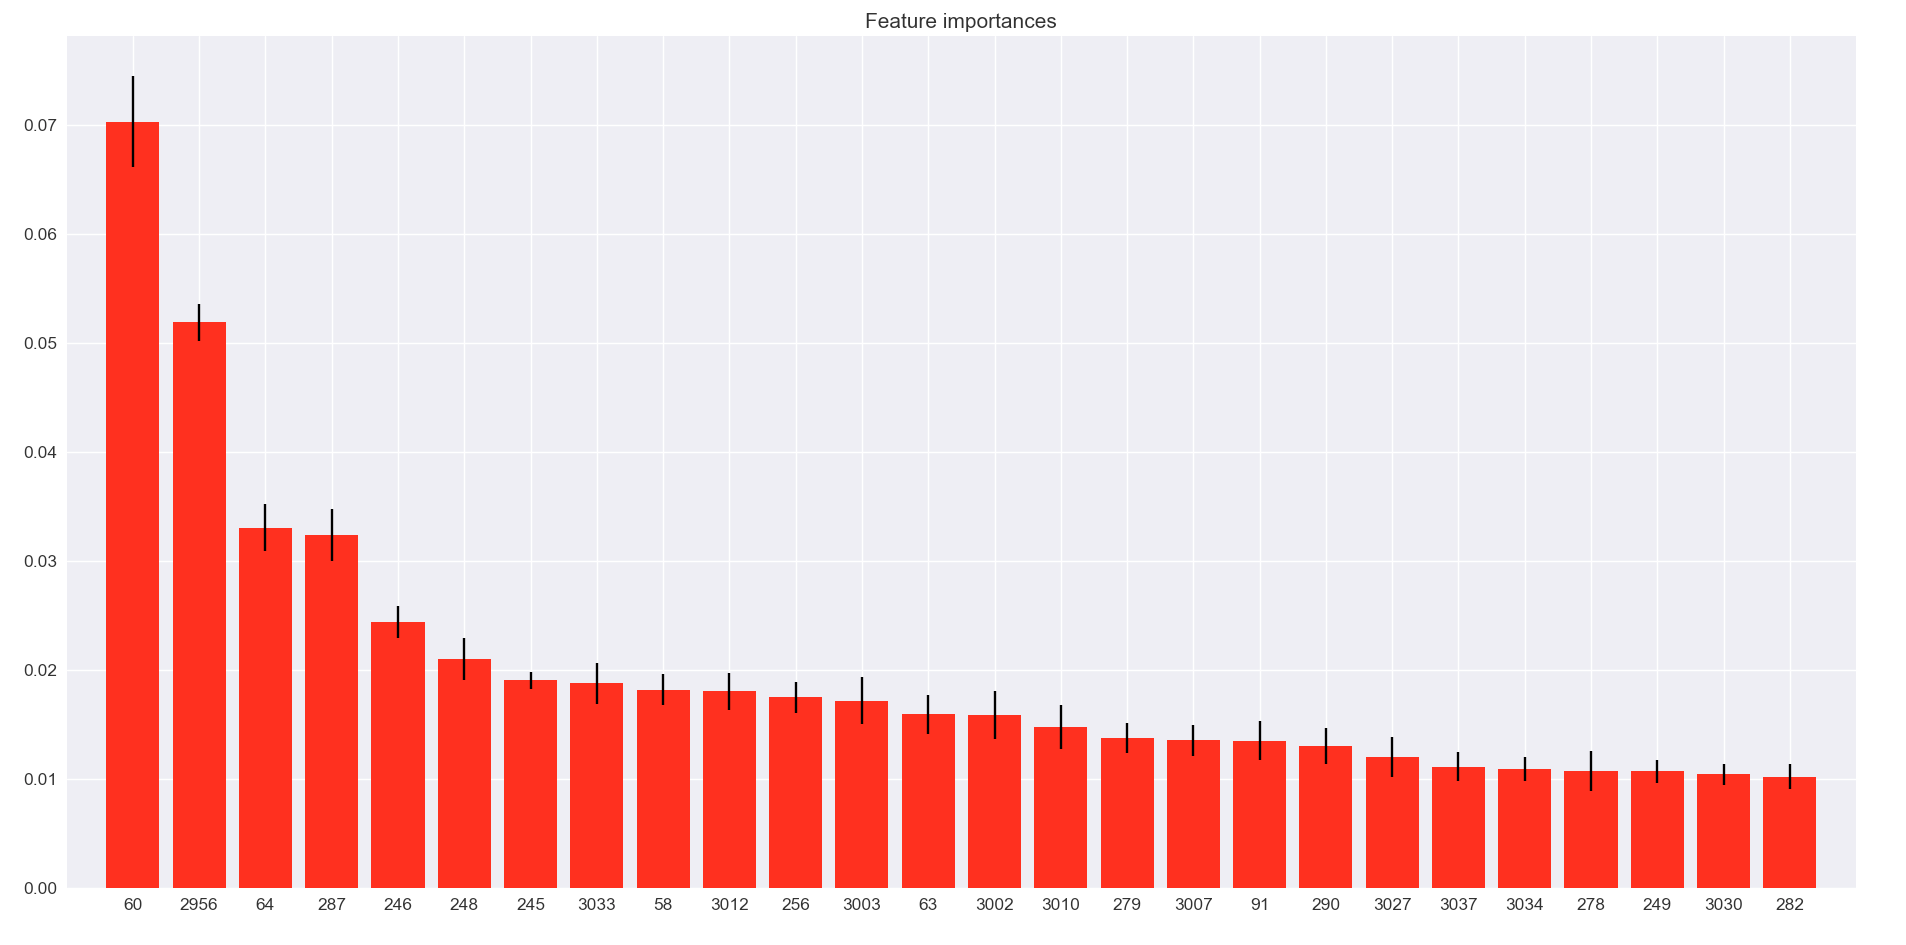
\includegraphics[width=\linewidth]{images/anhang/ml/Feature_importance_Tree.png}
  \caption{Feature Importance} 
\end{figure}

\begin{figure}[h]
  \centering
  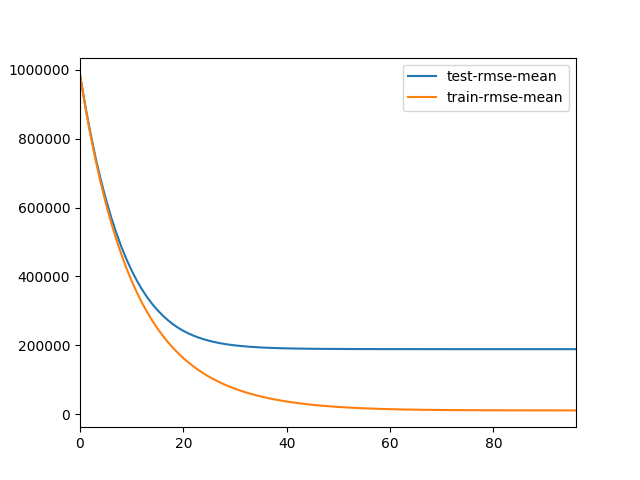
\includegraphics[width=\linewidth]{images/anhang/xgboost.png}
  \caption{XGBoost GridsearchCV} 
\end{figure}